% REMEMBER: You must not plagiarise anything in your report. Be extremely careful.
\documentclass{l4proj}

    
%==============================================================================
% Put any additional packages here
% You can add any packages you want, as long as it does not alter
% the overall format (e.g. don't change the margins or the reference style).
%
\usepackage{pdfpages} % if you want to include a PDF for an ethics checklist, for example
\usepackage{booktabs}
\usepackage{placeins}
\usepackage{enumerate}
\usepackage[shortlabels]{enumitem}

%
%

\begin{document}

%==============================================================================
%% METADATA
\title{Predicting Social Anxiety with Application Session Usage Data} % change this to your title
\author{Anguel S. Hristozov}
\date{March 31, 2020}

\maketitle

%==============================================================================
%% ABSTRACT
\begin{abstract}
    Social anxiety is a mental health disorder that affects a large portion of the population. Many individuals are not aware that they have it or refuse to seek help. Additionally, many health care systems around the world are not prepared to deal with the increasing number of individuals with social anxiety. It would be beneficial to try to lighten their workload by being able to provide assistance to these individuals.
    
    Smartphones have a large array of sensors that can be used to gather data. This includes location and mobility data, for example. Past research has shown that data gathered from these methods can be effective in identifying individuals with cognitive impairment as well as social anxiety.
    
    This project aimed to develop an accurate method of identifying socially anxious individuals based on the application usage session data. This data is essentially the applications that individuals use whenever their smartphone is unlocked. Additionally, the project compared gathered location data with previous research.
    
    A decision tree model was created with the location data and compared to past research. It was concluded that location data can be a good indicator of social anxiety but it should not be used by itself.
    
    Three different models were trained from the application usage session data. This was a decision tree, an extra trees, and a random forest classifier model. The decision tree produced the highest accuracy -- 93\%. The extra trees and random forest models achieved 86\% and 87\% accuracy, signifying that the decision tree may be subject to overfitting and other data related issues. It was concluded that application usage session data can be considered a good indicator of social anxiety, but more research needs to be done to confidently prove this.
\end{abstract}

%==============================================================================
%% ACKNOWLEDGEMENTS
\chapter*{Acknowledgements}

I would like to thank Professor Matthew Chalmers for his support and encouragement throughout this project. He challenged me with a lot of ideas and was always friendly in meetings. I would also like to thank my parents for being there throughout the whole process. Finally, I would like to thank the user trial participants for their patience and help.

%==============================================================================

\def\consentname {Anguel Hristozov} % your full name
\def\consentdate {31 March, 2020} % the date you agree
%
\educationalconsent


%==============================================================================
\tableofcontents

\chapter{Introduction}
This chapter will introduce the topic of mental health and look at the prevalence of social anxiety. The motivation for researching this topic will be explored as well as the project aim. Further chapters will explore the background information, design, implementation, evaluation, and conclusion.

% reset page numbering. Don't remove this!
\pagenumbering{arabic} 


\section{Motivation}
Mental health is a persistent issue in modern society. Besides adversely affecting an individual's daily life and health, mental disorders can predispose them to other serious diseases such as cancer, cardiovascular disease, and infections \citep{2013_mental_health_who}. In the United Kingdom alone, \citet{2005_mental_health} stated that one in ten young children aged 10-16 had a clinically diagnosed mental disorder. This statistic increased to one in six \citep{2007_mental_health_} and later to one in four \citep{2016_mental_health_report} throughout the years. An alarming aspect is that half of all the mental health problems in an individual are established by the age of 14 \citep{2016_mental_health_report} and may not be caught or may be accepted as normal behaviour. Individuals may feel social stigma or isolation \citep{2019_isolated} and may avoid treatment. Yearly investments in the United Kingdom National Health Service (NHS) to handle individuals with mental health increases every year \citep{2007_mental_health_costs, 2012_mental_health_costs}, and 13 billion pounds are planned to be spent alone in 2019/20, which are equivalent to 14\% of local NHS funding allocations \citep{2020_mental_health_statistics_funding}. Additionally, waiting times can vary \citep{2020_mental_health_statistics_waiting_time} and prevent individuals from getting help when needed.

Outside of the United Kingdom, the most prevalent disorders were anxiety disorders \citep{2016_prevalent_disorder}. Mental health can also be considered one of the main contributors to the overall disease burden worldwide \citep{2019_isolated} and can occur to anyone. Additionally, people have a 40\%-60\% chance of premature death \citep{2013_mental_health_who} and many health systems have not adequately responded \citep{2013_mental_health_who} to deal with this issue. There has been improvement over the years, and research has been ongoing to try to find new ways of catching problems before they become serious.

Studies have explored various techniques in studying individuals and their mental health \citep{student_life_site, boukhechba, salmon, tracking_depression_college_using_phone, avoidance_behaviour}. Techniques range from hand-held sensors to in situ self-reports with passive data gathering applications to virtual reality systems. These techniques have allowed researchers to get progressively closer to their subjects. A lot of research has utilised mobile smartphones, as their sensors allow for various data points to be collected. Mobile smartphones are also widely used, with 62\% of the world's population owning one \citep{bankcell}. These devices are also an integral part of many individual's lives \citep{digital_dependence, always_connected}, due to their quick availability for almost anything an individual may need. This makes them suitable for observing new behaviours and data that may not have been possible to achieve with previous technology.

With the increasing usage of mobile smartphones in research, more data can be gathered and converted into insightful conclusions. This can lead to quicker diagnosis, instant care, and other prevention methods to help combat mental health problems.

\section{Aim}
This project aims to see if an individual's Social Interaction Anxiety Scale (SIAS) score can be predicted within a reasonable range by observing the way that they use their mobile smartphone applications. The Social Interaction Anxiety Scale is one way to show if an individual exhibits symptoms of social anxiety. We want to use this scale in conjunction with passively collected background data to see if our aim is possible. The data should be collected by an application and should not hinder the participant. 

The data that we want to collect will be the application session data. This includes the applications they open, the categories of said applications, and how long each application was used during a single session. A session is defined as the time when a device is unlocked. We want to use this data to train a model to predict if an individual has social anxiety. Furthermore, we want to explore how the model will perform compared to other classifiers and determine if it would be viable to continue research into using application session data.

In addition to the main aim, we want to examine how accurate location data can be by comparing our model with previous related research. Our model will have different parameters and user trial length, and so we want to see if it would be feasible to use this configuration to train a model.

\section{Summary}
This chapter provides a brief introduction as to why we chose social anxiety as the research topic. We show some statistics for the United Kingdom as well as the rest of the world and discuss how research has progressed in this field. Ultimately we conclude that a smartphone is an appropriate technique for gathering data and how it compares to other methods, such as hand-held sensors and virtual reality systems. The remainder of this paper will discuss how requirements were gathered and implemented, and then how the data was evaluated and what conclusions we came to. The paper is structured as follows:
\begin{itemize}
    \item \textbf{Chapter \ref{Background}} gives more background information about social anxiety and its history. The Social Interaction Anxiety Scale mentioned above is explained in further detail. Professional related research is explored as well as past student dissertations.
    \item \textbf{Chapter \ref{requirements}} outlines the requirements for the study. A list of functional and non-functional requirements are presented as well as their justification.
    \item \textbf{Chapter \ref{design}} discusses the design process of each section of the project. Each design decision is related to the project requirements.
    \item \textbf{Chapter \ref{implementation}} reviews the implementation of the designs. It highlights the software engineering processes involved as well as what tools were used and why.
    \item \textbf{Chapter \ref{evaluation}} provides an evaluation of the model for predicting the SIAS score. This chapter also includes an examination of location data with past research.
    \item \textbf{Chapter \ref{conclusion}} summarises the report and lists any future work that could be performed.
\end{itemize}


%==================================================================================================================================
\chapter{Background} \label{Background}
This chapter examines what social anxiety is and provides statistics about how it affects the United Kingdom as well as the world. The Social Interaction Anxiety Scale (SIAS) is discussed and compared to other scales. Additionally, past research about social anxiety is provided, which includes previous student dissertation reports.

The term "social phobia" is used interchangeably in the diagnostic and statistical manual of mental disorders \citep{dsm_5}. In this study, we will use the term "social anxiety". Additionally, to avoid any further confusion, we will consider social interaction anxiety and social anxiety as one and the same, and will refer to the scale as either SIAS or the Social Interaction Anxiety Scale.

\section{Social Anxiety}
Social anxiety is defined as an overwhelming fear of social situations that does not go away on its own and can adversely affect many aspects of an individual's life \citep{nhs}. Individuals often have an intense fear of being watched and judged by others in social situations \citep{nimh}. Many circumstances can trigger an individual's anxiety, including talking to individuals, talking to individuals of authority, public speaking, and public performance \citep{anxiety_cause}. While these situations may create some level of anxiety in many individuals who do not suffer from social anxiety disorder (SAD), it is important to note that those who do suffer from SAD experience a distinctly high level of anxiety \citep{anxiety_cause}. This can lead to individuals having lower levels of self-confidence, and in turn cause them to fear that they may not be interesting or coherent \citep{sias_origin}.

Social anxiety also has an economic burden. Individuals with social anxiety tend to have a lower economic status due to under-performing educationally, and tend to visit the public health system more often \citep{social_anxiety_economic_burden}. This can put a strain on a nation's health care system and lead to reduced efficiency. Research has been done to explore indirect effects as well \citep{cost_of_social_anxiety, cost_in_europe}. There is also a social stigma that follows social anxiety, and many individuals may not understand it or may feel ashamed and do not seek help \citep{ACARTURK2009421}. All of this can lead to negative long-term effects \citep{kings}. Various studies have been done to explore individuals with social anxiety and how they interact with the internet, including how they may react to online situations while remaining anonymous and avoiding face-to-face interaction \citep{SHEPHERD2005949}. Additionally, technology is being used to simulate and analyse how socially anxious people deal with situations that require engagement \citep{avoidance_behaviour}.


\section{Social Interaction Anxiety Scale}
The Social Interaction Anxiety Scale (SIAS) was developed by \cite{sias_origin_unpublished, sias_origin}. It is a measure of an individual's social anxiety and is a self-report scale in the form of twenty questions (Appendix Figure \ref{fig:sias_questions}). Each question is rated on a five-point Likert scale \citep{sias_origin}, and answers range from "Not at all" to "Extremely". Each question is related to some sort of social interaction, and, except for questions 5, 9, and 11, a higher score can relate to a higher level of social anxiety. The range of scores is 0 to 80. A score of 34 and above indicates traditional social anxiety \citep{sias_score_34}.

Similar scales have been developed and evaluated to measure social performance e.g. the Social Phobia Scale \citep{sias_origin_unpublished, sias_origin, phobia_1, phobia_2, phobia_3}, the Social Avoidance and Distress Scale, the Fear of Negative Evaluation Scale \citep{1969_scales, heimberg_scales}, and the Social Phobia and Anxiety Inventory \citep{social_phobia_anxiety_inventory, inventory_anxiety}. These scales have suffered various criticisms, including the SIAS scale. Its limitations are that subjects are able to falsify responses \citep{sias_origin}, there can be response bias due to the questions being scored in the same direction \citep{sias_origin}, and that it can be hard to differentiate between users that have social anxiety and those that have generalised anxiety disorder \citep{phobia_2}.

In spite of its criticisms, the SIAS scale has been validated in multiple further studies. It has a normal distribution of scores \citep{sias_origin}, has internal consistency \citep{sias_origin, comparing_sias_sps, consistency}, and has high test-retest reliability \citep{sias_origin}. The internal consistency means that the different questions are correlated and produce similar scores as they measure social anxiety, and was assessed with Cronbach's alpha measure\footnote{\url{https://data.library.virginia.edu/using-and-interpreting-cronbachs-alpha/}}. The high test-retest reliability means that the scale will continue to correctly identify social anxiety in an individual after time has passed. The scale also has high discriminant validity \citep{consistency} and is able to differentiate between types of social anxiety \citep{sias_origin, phobia_1}.

The SIAS scale was chosen for this study as it is reliable and valid. Additionally, previous related research \citep{boukhechba, boukhechba_2} has used it. We would like to maintain continuity in using it as well as be able to compare studies and methods with past research.

\section{Technical Research}
This section will examine past research that is relevant to social anxiety and mental health. This is to provide an insight into general topic studies and how their results could be used in narrower studies that are only about social anxiety. These studies could be considered land-mark studies as they show the feasibility of using phone-based sensors to gather data that can be used to make valid conclusions. 

\subsection{StudentLife Study} % 2014
The StudentLife Study, done by Dartmouth College \citet{student_life_site}, was one of the first studies that explored how automatic and continuous data gathering can be used to examine the behaviour, performance, and mental health of a large student population. The study looked at students' mental health, grade point average, and behaviour during the course of a ten week term \citep{student_life_article}. 

The researchers used a combination of continuous sensor data and self-report questions. The sensor data was collected in the background while the self-reporting questions were asked at various times of the day. Sensor data included GPS, activity level, accelerometer, and proximity, among others. The self-report questions included surveys and Ecological Momentary Assessments (EMA). An EMA allows for the participants to report on their symptoms and behaviours shortly after experiencing them \citep{ema_description}. The results highlight the connection that exists between student mobility, activity level, sleep, and how it is a strong indicator of mental well-being \citep{student_life_article}. The idea of continuous background data collection is an important method that appears in many other studies and influenced us in our application design. 

\subsection{Next-Generation Psychiatric Assessment: Using Smartphone Sensors to Monitor Behaviour and Mental Health} % 2015
The Next-Generation Psychiatric Assessment study by \citet{next_gen_sensors} aimed to examine if smartphone sensors can be considered reliable for assessing an individual's mental health. Expanding on \citet{student_life_article}, this study utilised EMAs and captured phone sensor data. This data was used to infer geospatial activity, kinesthetic activity, and sleep duration. Multiple sensors were used in conjunction to generate these higher-level features. \citet{understanding_mental_healh_using_sensors_and_ml} argue that converting lower-level raw data to higher-level features is much more valuable than just using the raw data by itself. Additionally, \citet{understanding_mental_healh_using_sensors_and_ml} shows that raw data can be used in multiple combinations to produce a variety of features. The study concluded that geospatial activity, kinesthetic activity, and sleep duration data is able to be used for analysing user mental health, daily stress, and levels of depression. The study also showed that it is enough for data to be collected passively without requiring further user interaction. This further influenced us to use passive background data collection.

The following study by \citet{mobile_sensing_for_depression_social_anxiety} looked at how analysing location data gathered by mobile phone sensors coupled with in situ self-report questions relate to mental health. Specifically, the study looked at the relation between staying at home and depression and social anxiety. Various temporal windows were examined, and the study concluded that higher social anxiety was linked to more time spent being home \citep{mobile_sensing_for_depression_social_anxiety}. This study is important because it shows the feasibility of using location data to understand a person's state of mental health. This influenced us to collect location data to compare it to past research and observe the results.

Another study by \citet{tracking_depression_college_using_phone} expands by proposing a new approach to predicting depression. The researchers created a set of symptom features that proxy the DSM-5 defined symptoms \citep{tracking_depression_college_using_phone}. These are made specifically for college students. With this method, the researchers were able to show changes in the students' depression on a week by week basis. This is significant because it allows for actionable change by college professors and administration. If they have an insight into how students are feeling on a week by week basis then they would be able to react and adjust accordingly to help them cope. This study influenced us to research the topic of social anxiety.


\subsection{Monitoring Social Anxiety from Mobility and Communication Patterns} % 2017
The Monitoring Social Anxiety from Mobility and Communication Patterns study by \citet{boukhechba} had a more focused approach than StudentLife in regards to what was researched. They focused on mental health, specifically social anxiety, and how it relates to passively collected GPS location data and communication patterns (calls and SMS texts). This data was paired with respective SIAS scores to explore the feasibility of using such sensor data to predict the social anxiety level.

This study is significant because of the high accuracy in predicting social anxiety based on location and mobility patterns, which are common data points and trivial to acquire. The research showed that mobility (location) patterns alone gave a prediction accuracy of 77\%. When combined with communication patterns, the accuracy increased to 85\%. A C4.5 decision tree algorithm was used during the data analysis. A significant difference between this and StudentLife study is that \citet{boukhechba} did not use EMA but instead asked the participants to take the SIAS self-report once. This is less demanding of users and meant that the passively collected data was enough to predict. This choice had a strong influence on how we chose to implement the SIAS self-report aspect.

\subsection{Predicting Social Anxiety From Global Positioning System Traces of College Students: Feasibility Study} % 2018
\citet{boukhechba_2} aimed to explore if GPS location could assess college students' social anxiety levels. Unlike the previous study by \citet{boukhechba}, communication (calls and SMS texts) were not collected. A SIAS test was administered at the very start of the study before the data collection application was installed. This influenced our implementation to have the SIAS test administered before the data collection was turned on.

Location data was aggregated into clusters and then associated with a semantic label. Various features were extracted from the processed data, including duration of visits, location entropy, and the frequency of transitions \citep{boukhechba_2}. The study shows that students with a high social anxiety level tend to avoid locations that are social in nature, such as restaurants or bars. This study is significant because it showed that location data alone can give a lot of insight into a person and their social anxiety level. The method of assigning semantic labels to data locations had a strong influence on how we chose to post-process our location data into category labels.

\subsection{A Large-Scale Study of iPhone App Launch Behaviour} % 2018
The Large-Scale Study of iPhone App Launch Behaviour by \citet{apptracker} reported on how iPhone users compare and contrast with their Android counterparts. The study recognised that mobile phone application launch behaviour research mainly used Android devices and aimed to reproduce several of these studies but with iPhone users. They conclude that while some differences exist, significant similarities are present: communication applications are the most used on both systems, few applications are very popular on both systems, and almost identical proportions of people use a unique combination of applications \citep{apptracker}. This is important, as it shows that studies done with Android users could, for the most part, apply to iPhone users as well. \citet{angry_birds_study} in an earlier study showed various patterns and statistics in application usage. They discussed application usage chains and how certain categories are popular during certain parts of the day. The study was done on Android devices. \citet{welke} showed that it is possible to differentiate between users based on their application signature, which is their set of used applications. The study states that there is a unique signature for 99.67\% of users, which has serious implications on privacy. This includes weak permission settings on phones in regards to what data applications are able to gather. Additionally, it further implies that individuals can be easily identified by their application signature.

\citet{apple_patterns} looked to expand upon the previously mentioned papers and analysed phone usage data to try to reveal differences in how people with and without cognitive impairments use their phones. The study looked at various application usage patterns. The data was split into application usage session, and sessions were clustered by their type. This allowed them to see the flow of application usage and further understand how applications relate to each other. The result was that application usage alone can capture systematic differences between healthy and cognitively impaired users \citep{apple_patterns}. This is important because it highlights the value of application usage, and further validates the research before it. This paper strongly influenced us to focus on application session data.


\section{Previous Student Dissertations}
This section will explore previous research on social anxiety that was conducted by University of Glasgow students. These students explored what kinds of data can be used to predict an individual's social anxiety. While smaller in scope than the research mentioned above, we believe that there are actionable conclusions presented.

\subsection{Dimitris Elftheriou Dissertation}
A student of the University of Glasgow, Dimitris Elftheriou, conducted a study that took inspiration from \citet{boukhechba} and used the AWARE Framework\footnote{\url{https://awareframework.com/}} to gather mobile phone data and determine if it is possible to predict an individual's social anxiety levels. The AWARE project was created to be a reliable and implementable data collection framework for researchers to apply in their user-studies \citep{aware_thesis, aware}. \citet{dimitris} was able to achieve similar results to \citet{boukhechba} based on the same C4.5 decision tree algorithm. Additionally \citet{dimitris} created a framework to gather data responsibly and follow the GDPR guidelines. The implication of this is that less personally identifying data was given by the participants. We took influence from this by aiming to collect as little personally identifying data as possible. 

\subsection{Ryan Fox Dissertation}
A student at the University of Glasgow, Ryan Fox, conducted a study that assessed whether it was possible to detect SAD with non-identifiable information. The data collected was battery charge patterns (time spent in high/low battery level and time spent charging device) as well as activity data using the Google Location and Activity Recognition\footnote{\url{https://developers.google.com/location-context/activity-recognition/}} API. The results were inconclusive due to an inadequate data set produced by the Android application \citep{fox}.


\subsection{Edward Wood Dissertation}
A student at the University of Glasgow, Edward Wood, conducted a study that aimed to expand on \citet{student_life_article, boukhechba, dimitris} and create a less intrusive application to limit required user input \citep{wood}. \cite{wood} gathered location data and clustered the locations into categories using the Google Maps\footnote{\url{https://developers.google.com/maps/documentation}} and Open Street Map\footnote{\url{https://wiki.openstreetmap.org/wiki/API}} libraries. The study showed that the generated model had high accuracy in predicting an individual's SIAS score by using location categories \citep{wood}.

\section{Summary}
This chapter discussed previous research that explored cognitive health in individuals and how it can be tracked and predicted by sensor data. Various data gathering techniques were shown, including hand-held sensors and smartphones. Research about social anxiety was discussed, and we explained how past research has been able to link location data as well as application session data to social anxiety and other forms of cognitive impairments. We talked about how the research influenced our project design and implementation.
 
%==================================================================================================================================
\chapter{Analysis/Requirements} \label{requirements}
% talk briefly about what this section will be about, including how requirements were gathered
This project was presented by Matthew Chalmers, a University of Glasgow professor and researcher. The aim was to expand on previous research that he supervised in relation to social anxiety. 

\section{Problem Analysis}
This project aims to see if an individual's Social Interaction Anxiety Scale score can be predicted within a reasonable range by observing the way they use their mobile smartphone applications. To accomplish this, we need to create a mobile application that can passively collect background data. Additionally, we need the application to allow the participant to take the SIAS quiz.

The collected data needs to be analysed and used to train a classifier to predict if a participant exhibits socially anxious tendencies (SIAS score at or above 34) or does not (SIAS score below 34). This classifier then must be validated to check its accuracy and performance. Additionally, the collected location data must be compared with previous research.

The data must be stored securely and the participants need to be kept aware of how their data is to be used. General data protection regulation guidelines \citep{gdpr_guidelines} need to be followed. At all steps, the participant must be in control of their data and be able to opt-out. Additionally, a user should not be explicitly linked to their data, and so a random unique identifier must be assigned for the sole purpose of linking the SIAS score to the respective data.

\section{Requirements}
An iterative approach was used to gather requirements. Each meeting with the supervisor was considered an iteration. These early iterations were vital in setting the direction and were used to gather the base requirements and overall aim of the project. The sections below will describe the functional and non-functional requirements that were gathered. %Different requirements were set for the mobile application and the data analysis, and so will be listed separately.

\subsection{Functional Requirements}
The MoSCoW \footnote{\url{https://www.agilebusiness.org/page/ProjectFramework_10_MoSCoWPrioritisation}} method of prioritising requirements was used to set deadlines and track progress. The MoSCoW method labels requirements by priority: 
\begin{itemize}
    \item \textit{Must Have} - describes requirements that are necessary for the project to succeed. If these are not met, the project is not viable.
    \item \textit{Should Have} - describes requirements that are important but are not directly related to the success of the project.
    \item \textit{Could Have} - describes requirements that are beneficial but do not have a negative effect if they are not implemented.
    \item \textit{Won't Have This Time} - describes requirements that are not implemented but are useful to clarify the current scope of the project.
\end{itemize}
The labels \textbf{M}, \textbf{S}, \textbf{C}, and \textbf{W} will represent \textit{Must Have}, \textit{Should Have}, \textit{Could Have}, and \textit{Won't Have This Time} in the requirements sections below. Each requirement will have the format \textbf{Number - Label - Met}, where the number is to keep track, label is one of the MoSCoW labels, and met will be in the set of \textbf{\{Y, N\}} where \textbf{Y} means that the requirement was met and \textbf{N} means that it was not.

\subsubsection{Application} \label{mobile-app-reqs}
\begin{enumerate}[start=1,label={\textbf{\arabic* -}}]
    % MUST HAVES
    \item \textbf{M - Y} Allow user to take SIAS exam. The score must be saved onto the device. This is necessary to be able to link the data with a score.
    \item \textbf{M - Y} Keep application alive. There must be a service to prevent the application from begin killed when it is not in the foreground or being used. This is necessary to ensure data is collected in the background.
    \item \textbf{M - Y} Track session usage. Each session must be saved onto the device. This is necessary to be able to see what applications were used in each session.
    \item \textbf{M - Y} Restart the application if the device restarts. This is necessary to ensure that data collection resumes without a large interruption.
    % SHOULD HAVES
    \item \textbf{S - Y} Track call duration. Each phone call should have its duration saved. This is important to be able to compare with past research.
    \item \textbf{S - Y} Export the data to an external database. This is important as it allows the participant to export the data whenever they are able to instead of having to manually export it to a file and then send.
    \item \textbf{S - Y} Allow for data collection to be toggled on and off. This is important as there may be certain situations when participants may not want it on, such as when the battery is low.
    \item \textbf{S - N} Restart the application if it crashes unexpectedly. This is important as the device may have run out of memory or is really aggressive with management.
    \item \textbf{S - N} Track text message data. Each text message should have some data about it saved. This is important to be able to compare with past research.
    % COULD HAVES
    \item \textbf{C - Y} Allow the participant to opt-out from the app. This is useful to have so that the participant does not need to directly contact the researcher but instead anonymously send their identifier and have it excluded from the collected data.
    \item \textbf{C - N} Activity recognition. This could have been beneficial in augmenting the session data to see what the participant was doing at the time of usage. We did not have enough time for this.
    % WOULD HAVES
    \item \textbf{W - N} Do data processing on the phone and use federated machine learning from each participant device. This would have been useful to ensure that the data did not leave the device. We did not have enough time for this.
\end{enumerate}

\subsubsection{Data Analysis}
\begin{enumerate}[resume,label={\textbf{\arabic* -}}]
    % MUST HAVES
    \item \textbf{M - Y} Fix unknown categories and application names. This is because some applications do not have a category assigned to them.
    \item \textbf{M - Y} Perform decision tree classifier validation. This is to ensure the validity and accuracy.
    % SHOULD HAVES
    \item \textbf{S - Y} Compare the decision tree classifier with more advanced classifiers. This is to see if there are any issues.
    \item \textbf{S - Y} Compare results from past research with our own results. This is to see its validity as well as how it changes.
    % COULD HAVES
    \item \textbf{C - N} Find the best classifier with the best parameters. We did not have time for this.
    % WOULD HAVES
    \item \textbf{W - N} Have an interactive prompt for the data analysis script. We did not have enough time for this.
\end{enumerate}

\subsubsection{Server and Database}
\begin{enumerate}[resume,label={\textbf{\arabic* -}}]
    % MUST HAVES
    \item \textbf{M - Y} Encrypt the data at rest and at transit. This is necessary to safeguard the data.
    \item \textbf{M - Y} Encrypt the communication between the application and server. This is necessary to keep the data encrypted when it is being sent from the device.
    % SHOULD HAVES
    \item \textbf{S - Y} Try to ensure that the data only comes from the application and participants without requiring any personal details. This is important as the server URL will be public.
\end{enumerate}

\subsection{Non-Functional Requirements}
The non-functional requirements relate to application performance and usage but are not explicitly required for a viable product. Their goal is to aid the performance and give the participant more transparency. The MoSCoW method was used to prioritise, and they are listed below in the same format as above.

\subsubsection{Application}
\begin{enumerate}[resume,label={\textbf{\arabic* -}}]
    % MUST HAVES
    \item \textbf{M - Y} Allow the participant to see the data collected. This is necessary to be transparent and account for regulations.
    \item \textbf{M - Y} Have little to no impact on battery life. This is necessary to make sure the application does not cause any inconveniences.
    % SHOULD HAVES
    \item \textbf{S - Y} Integrate with a build system to build the application. This is important as it would allow participants to download the application file for their device.
    \item \textbf{S - N} Encrypt the data on the device. This is important in case someone else acquired access to the participant phone.
    % COULD HAVES
    \item \textbf{C - Y} Add option for participant to learn about the SIAS exam.
    \item \textbf{C - Y} Integrate with an application crash tracking service. This would aid in debugging issues.
    % WOULD HAVES
    \item \textbf{W - N} Collect extra data, for example from network usage. We did not have enough time for this.
\end{enumerate}

\subsubsection{Server and Database}
\begin{enumerate}[resume,label={\textbf{\arabic* -}}]
    \item \textbf{M - Y} The server must not crash and must remain up during data upload.
    \item \textbf{M - Y} The server must prevent anyone besides the researcher from being able to log in.
    \item \textbf{M - Y} The database must be visible only from the server.
\end{enumerate}

\section{Summary}
This chapter described in detail the requirements that were gathered for the project. It split them into functional and non-functional. The requirements were then further categorised by the MoSCoW system. Each requirement is justified as to why it was gathered.

%==================================================================================================================================
\chapter{Design}\label{design}
This chapter will describe the architecture and design of the mobile application and data analysis platform. We will also look at the data analysis algorithms. Lastly, the server and database that were used to store the data will be examined. The GDPR guidelines (\cite{gdpr_guidelines}) were used to influence our design decisions.

\section{Mobile Application}
This section will discuss the mobile application architecture designed independently of the underlying device operating system. The user interface will be discussed afterwards.

\subsection{System Architecture}
The application architecture diagram\footnote{All diagrams in this chapter, with the exception of wireframes, were created with diagrams.net\url{https://www.diagrams.net/}, formerly known as Draw.io.} shown in Figure \ref{fig:app_system_diagram} can be broken down into several services. These are the data gathering, SIAS test, export, staying alive, and restarting service.

The participant engages with the SIAS test, data gathering, and export service. For all three, the participant must start them. This was done to let the participant understand that they are in full control, and allow them to back out if they chose to. These services were created from functional requirements in section \ref{mobile-app-reqs}, specifically \textbf{1}, \textbf{3}, \textbf{5}, and \textbf{6}.

The staying alive and restarting services are handled by the system, as they are critical for the application to run continuously. These services were created from functional requirements in section \ref{mobile-app-reqs}, specifically \textbf{2} and \textbf{4}. The staying alive service has the task to prevent the underlying operating system from killing the application. The restarting service has the task to start the application if the device is restarted. Both of these services had to be designed to be efficient and quick so that the system does not stop them.

The system architecture design does not take into account non-functional requirements. They are not required to ensure reliable data collection. Their implementation will be discussed later.

\begin{figure}[!htb]
    \centering
    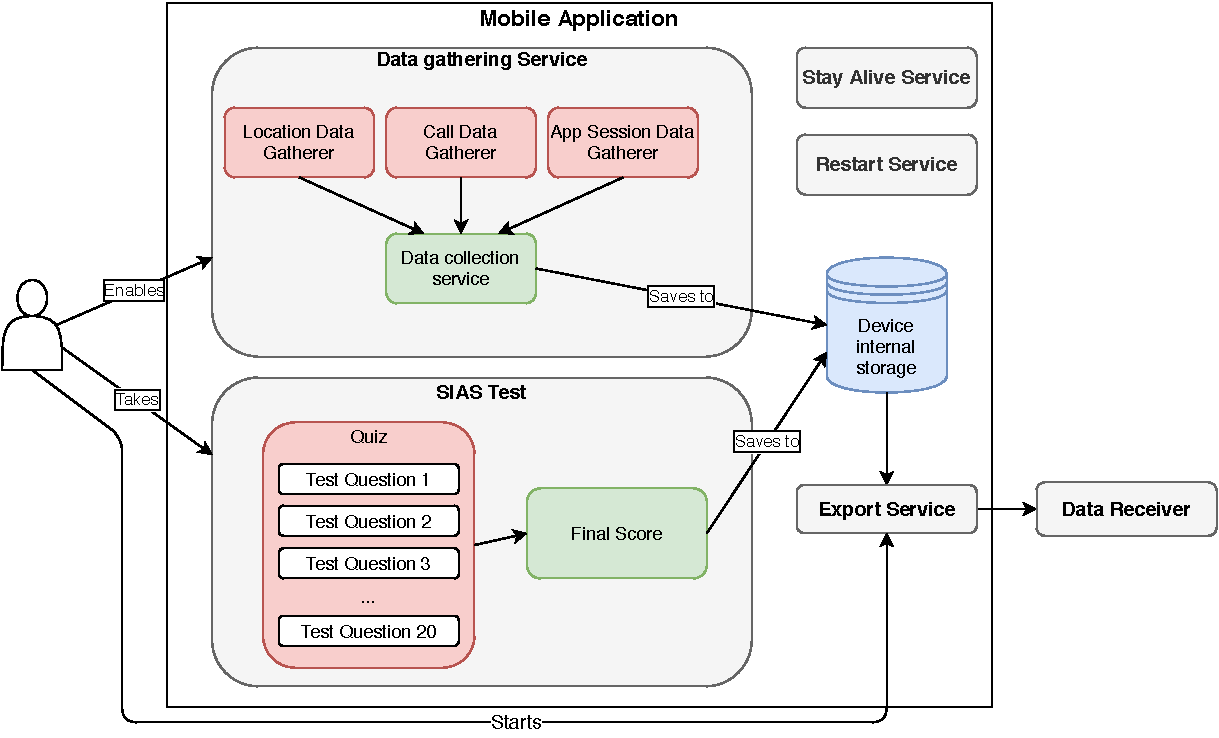
\includegraphics[width=0.95\linewidth]{images/app_system_diagram.pdf}    
    \caption{This figure shows the system diagram of the application. All of these services reside in the same application but we felt it necessary to split them up as to understand the entire system better.}
    \label{fig:app_system_diagram} 
\end{figure}
\FloatBarrier

\subsection{User Interface}
There were a few functional requirements that involved user interaction. As such, the user interface was designed to be as minimal and easy to use as possible. The interface design went through multiple iterations and feedback was gathered at various steps. The interface was guided by functional and non-functional requirements, specifically \textbf{7}, \textbf{10}, and \textbf{22}.

The interface needed to allow the user to directly interact with the services that required it. The wireframes\footnote{All of the wireframes in this report were created with the tool Balsamiq:  \url{https://balsamiq.com/}} of the initial prototype in Figure \ref{fig:initial_prototype_wireframes} show the four screens that would be visible to the user. The main screen in Figure \ref{fig:main_screen_1} is what the user would see when the application is launched. From there, the user would be able to take the SIAS test, as shown in Figure \ref{fig:test_screen_1}. If the user went to data collection from the main screen, the screen in Figure \ref{fig:data_screen_1} would allow them to toggle the collection on and off as well as see the data that has been collected. The settings screen in Figure \ref{fig:settings_screen_1} would allow the user to enable the relevant permissions and choose to opt-out.

We informally evaluated the initial application prototype ourselves after it was created. This guided us to modify the design to move all data to the settings screen and change the main screen, as shown in Figure \ref{fig:final_prototype_screen}. This decision was done so that there would be a central place where the participant could view their data, including their identifier and SIAS score, and it would be separate from the screen where data collection was controlled.

\begin{figure}[htbp]
    \centering
    \begin{subfigure}[b]{0.45\textwidth}
        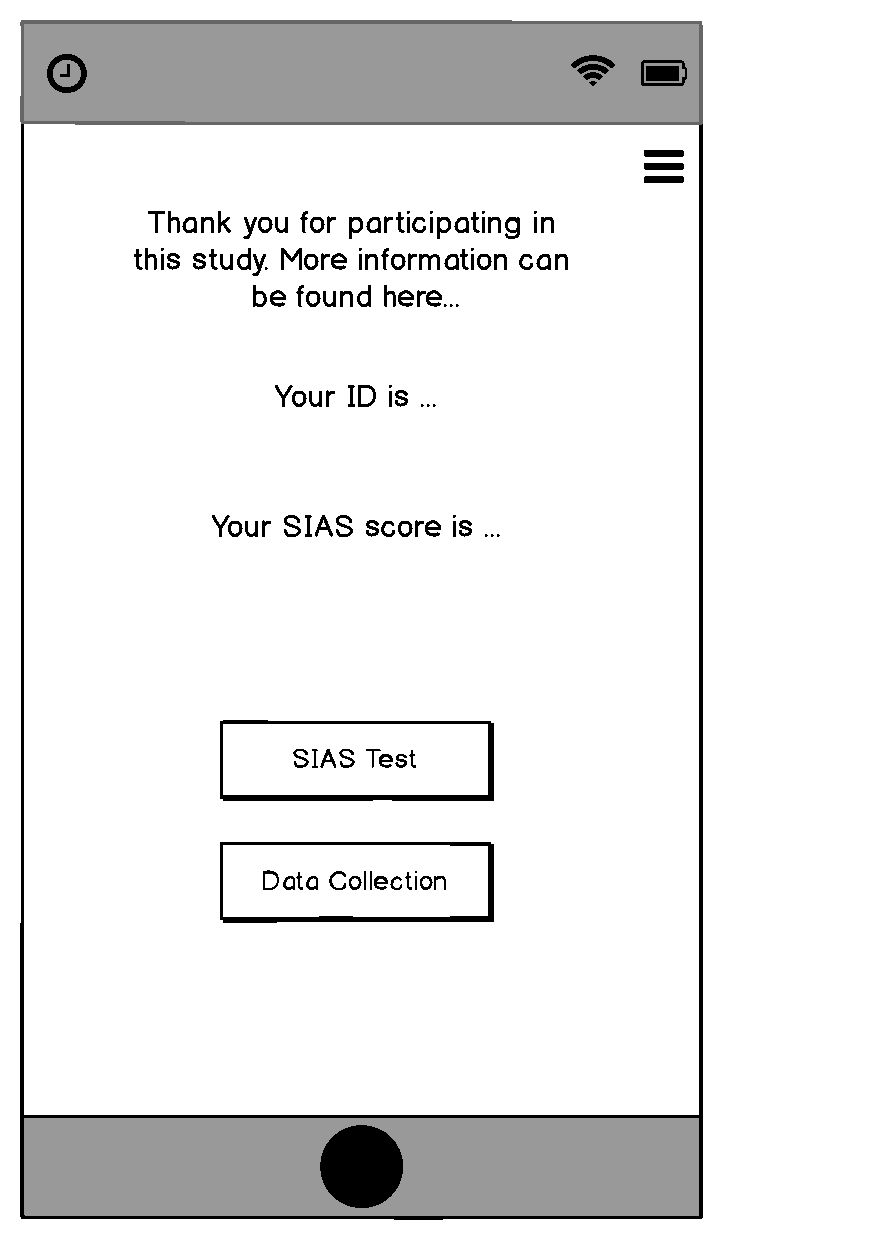
\includegraphics[width=\textwidth]{images/iteration_1_main_screen_1.pdf}
        \caption{Main Screen}
        \label{fig:main_screen_1}
    \end{subfigure}
    \begin{subfigure}[b]{0.45\textwidth}
        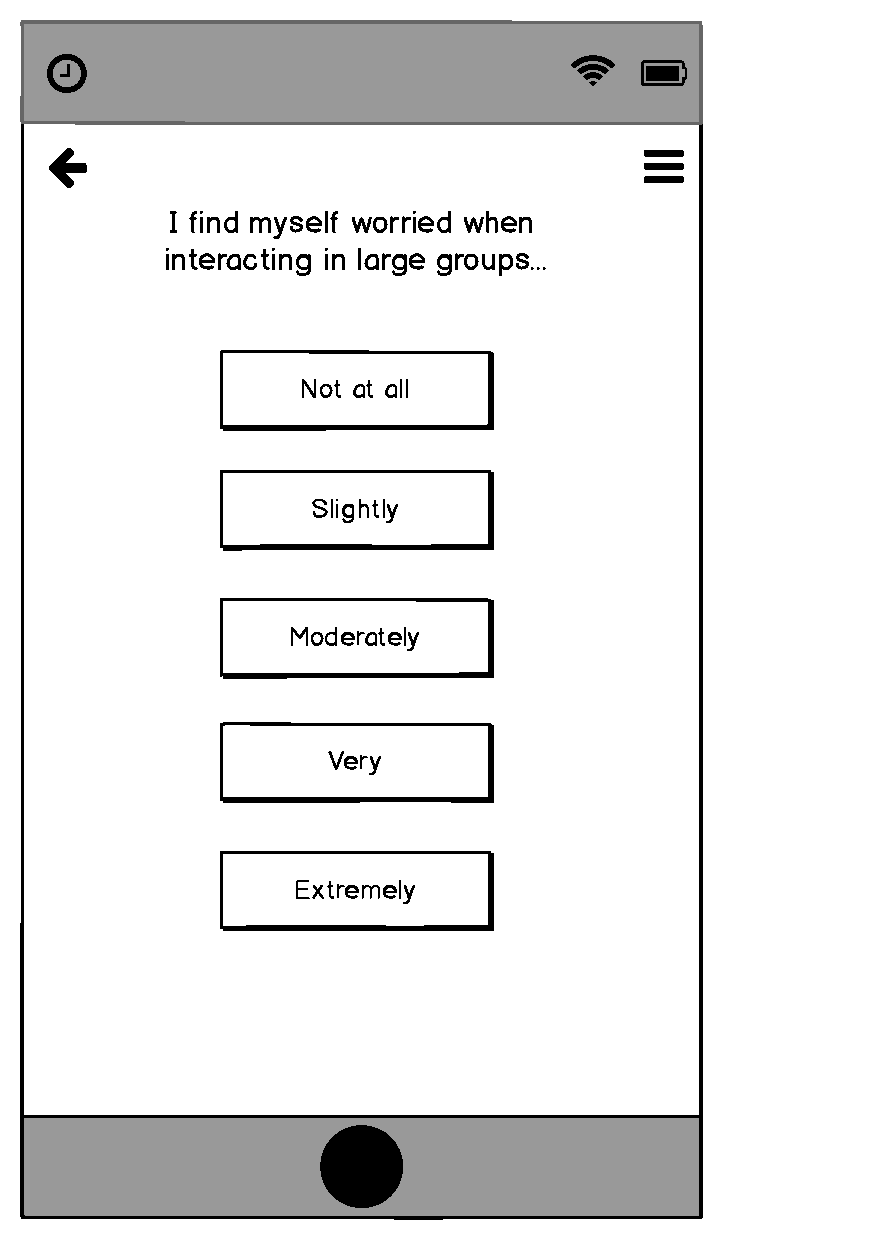
\includegraphics[width=\textwidth]{images/iteration_1_test_screen_1.pdf}
        \caption{SIAS Test Screen}
        \label{fig:test_screen_1}
    \end{subfigure}
    \begin{subfigure}[b]{0.45\textwidth}
        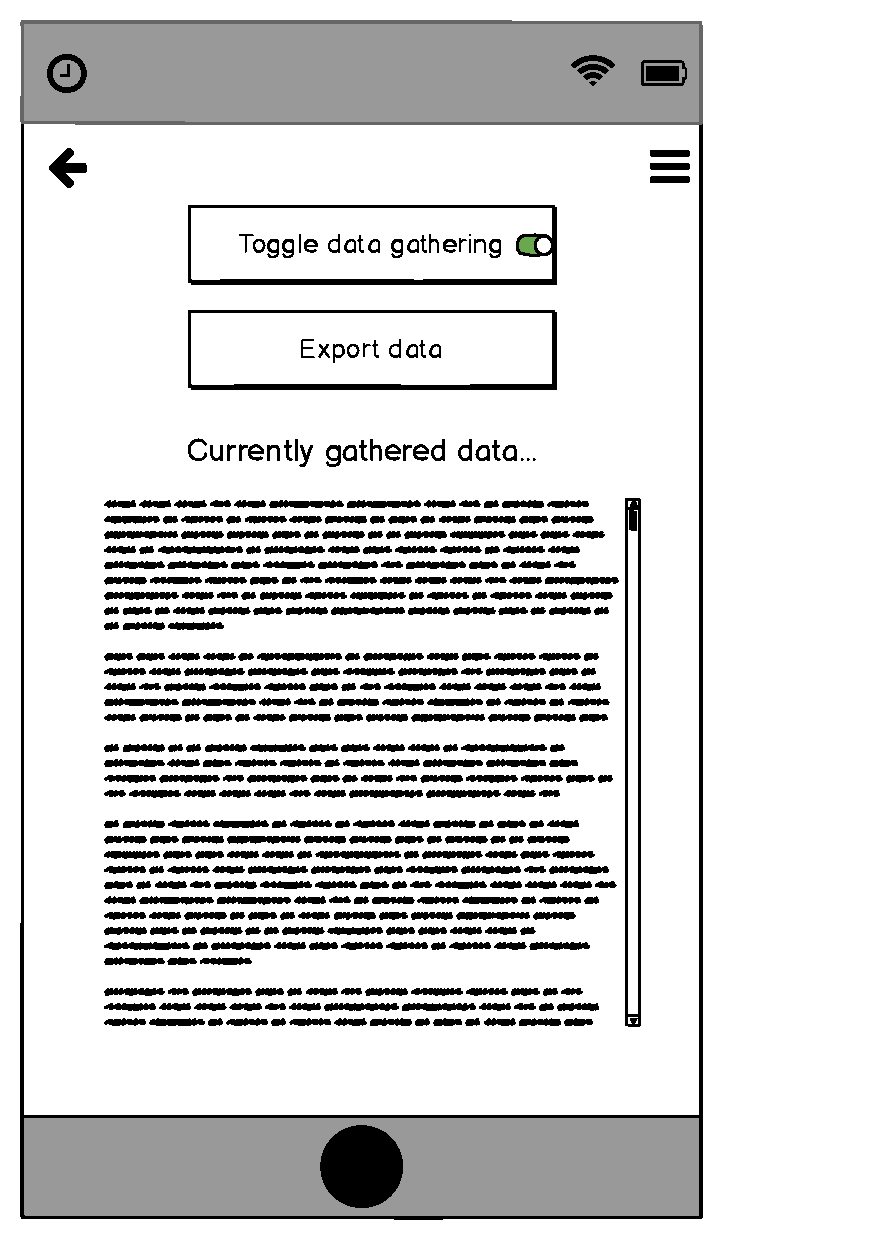
\includegraphics[width=\textwidth]{images/iteration_1_data_screen_1.pdf}
        \caption{Data Gathering Screen}
        \label{fig:data_screen_1}
    \end{subfigure}
    \begin{subfigure}[b]{0.45\textwidth}
        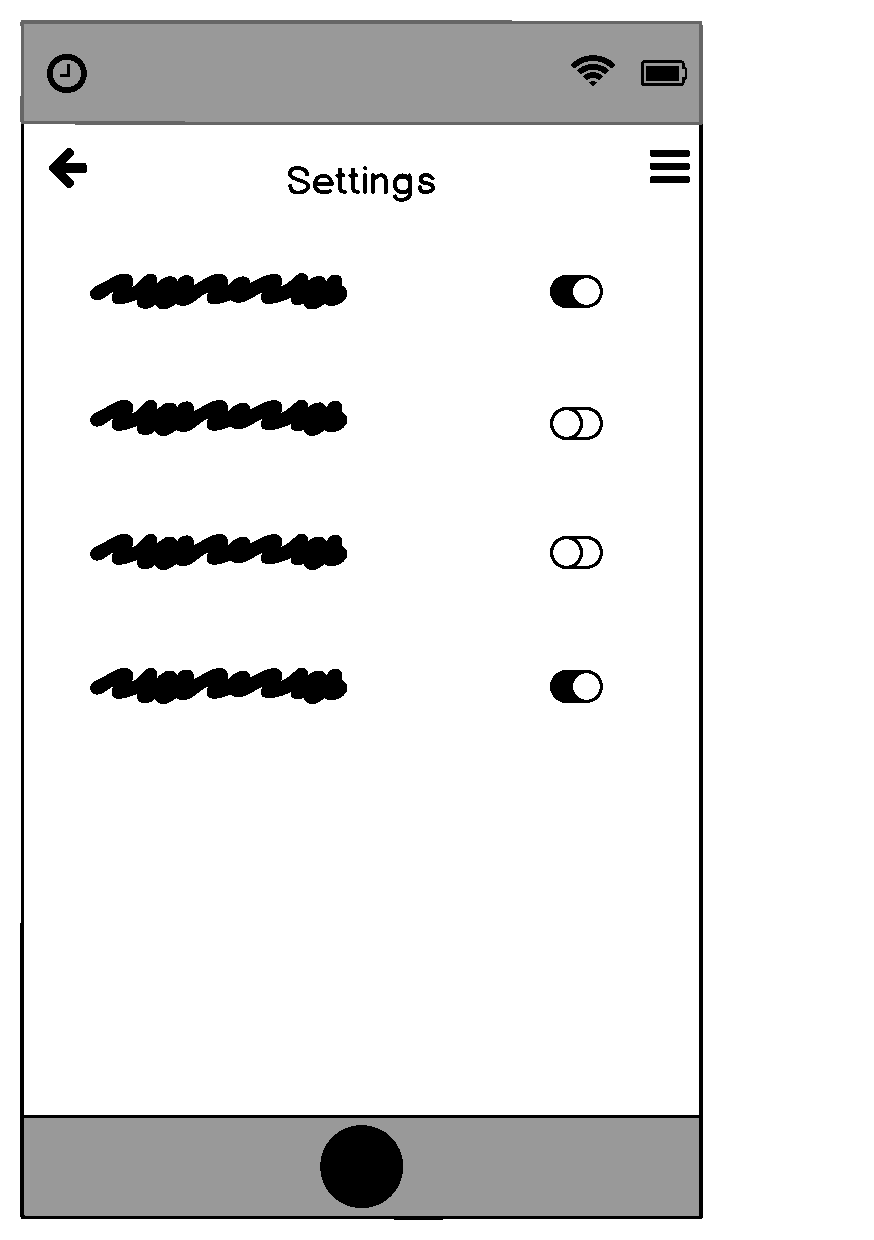
\includegraphics[width=\textwidth]{images/iteration_1_settings_screen_1.pdf}
        \caption{Settings Screen}
        \label{fig:settings_screen_1}
    \end{subfigure}   
    \caption{This figure shows the wireframes created for the initial application prototype.}\label{fig:initial_prototype_wireframes}
\end{figure}

\begin{figure}[htbp]
    \centering
    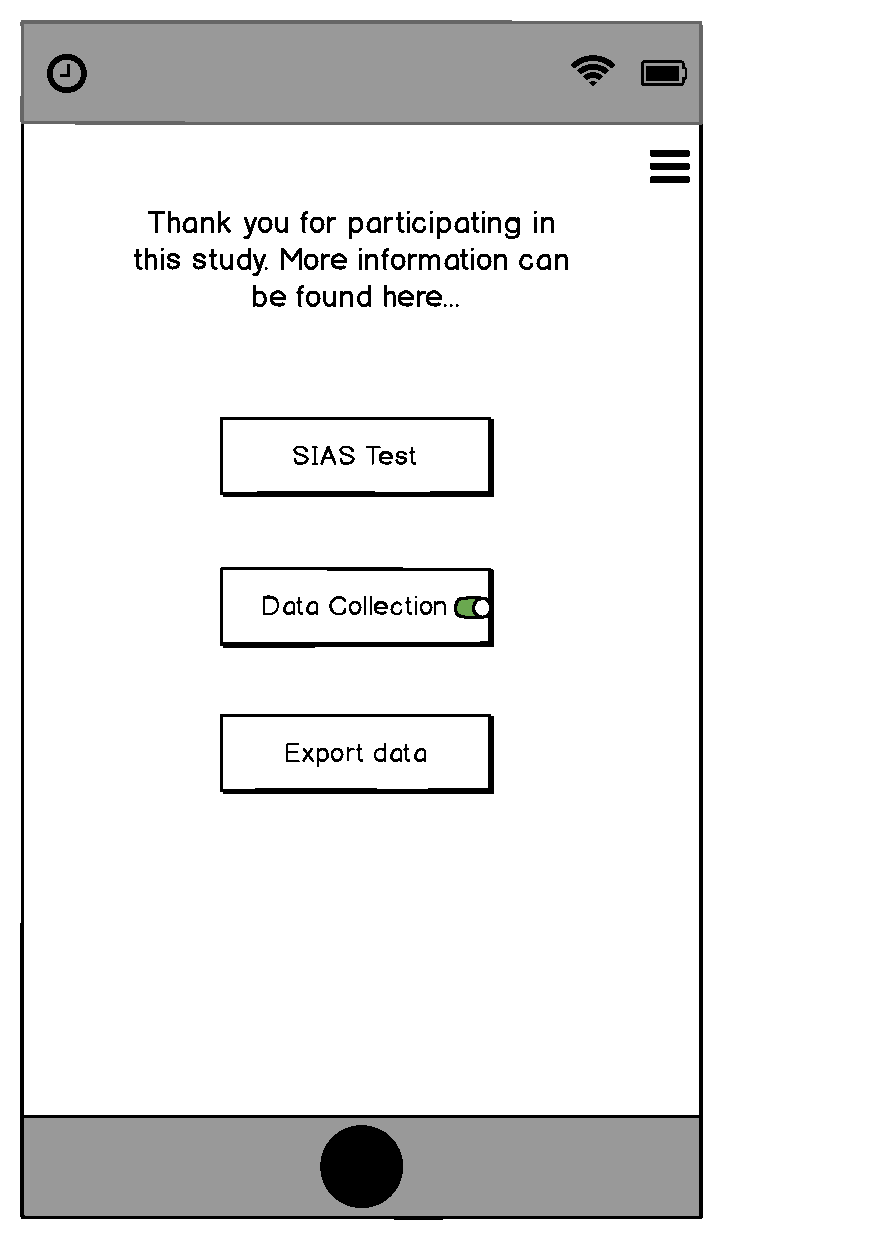
\includegraphics[width=0.40\linewidth]{images/iteration_2_main_screen.pdf}    
    \caption{The final design of the application main screen. It is important to note that the data collection screen shown in Figure \ref{fig:data_screen_1} was removed and instead an extra toggle button was added to the main screen. The text that notifies the participant of their identifier and SIAS score as well as the ability to view the data were removed. The test and screen settings in Figures \ref{fig:test_screen_1} and \ref{fig:settings_screen_1} respectively remain the same.}
    \label{fig:final_prototype_screen} 
\end{figure}


\section{Data Analysis}
The data analysis system must be able to read in the collected data, either from a database or local file. It should then process it and use it to train the decision tree classifier. Afterwards, various graphs and charts should be generated once the classifier is done training and has been validated. Figure \ref{fig:data_analysis_system} shows the architecture of the data analysis.

\begin{figure}[htbp]
    \centering
    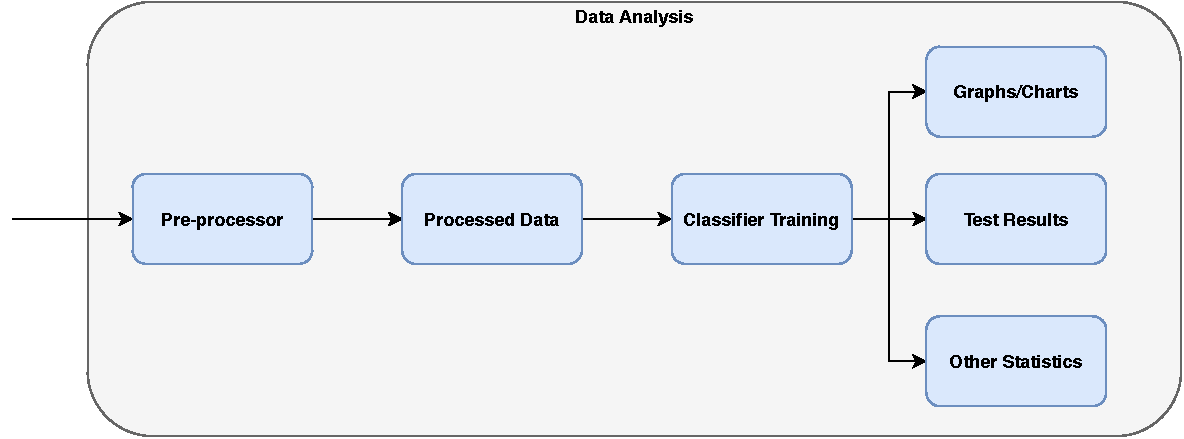
\includegraphics[width=0.80\linewidth]{images/data_analysis_system.pdf}    
    \caption{This figure shows the system architecture of the data analysis system. It is important to note that the flow of data is linear, and there is no interaction with the participant. This is simply for us to analyse the data once gathered.}
    \label{fig:data_analysis_system} 
\end{figure}


\section{Server and Database}
This section will discuss the server and database and their purpose. The server must receive the data from the application and then save it in a database. Figure \ref{fig:server_diagram} shows the architecture of both the server and database. The server is made of two services, a data receiver and processor. The receiver must handle as it comes in. Additionally it must be able to handle a high load in both requests and data. The processor must extract the data from each request and send it to the database to be saved. The architecture presented in Figure \ref{fig:server_diagram} is designed to be simple yet extensible.

The server is split into two services to ensure that there is no direct connection to the database from the application. It also allows for stricter control over firewall and network settings for both server and database.

\begin{figure}[htb]
    \centering
    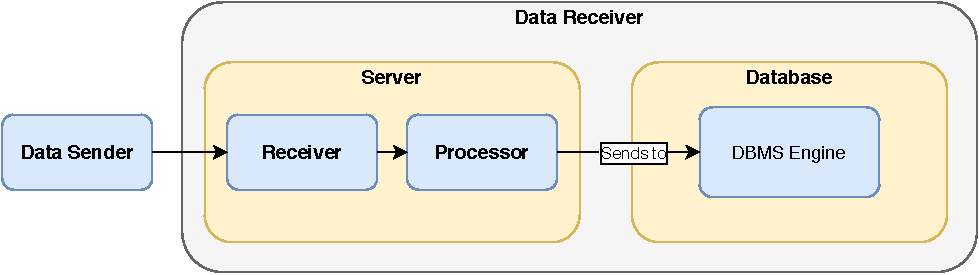
\includegraphics[width=0.80\linewidth]{images/server_diagram.pdf}    
    \caption{The architecture for the system that receives the exported data from the application. The application is not directly connected to the database, and so a middle layer, the server, must be used to receive, process, and send the data off.}
    \label{fig:server_diagram} 
\end{figure}


\section{Summary}
This chapter looked at the overall design of the various parts of the project. The application was explained in great detail about what functionality it should have and how the user should interact with it. This includes both the background data processing and the user interface aspect. Next, the chapter looked at the data analysis system and its purpose of producing graphs, metrics, and classifier models using the gathered data. Finally, the database and server section looked at the role of storing the data remotely.


%==================================================================================================================================
\chapter{Implementation} \label{implementation}
% What did you do to implement this idea, and what technical achievements did you make?
This chapter will discuss how the designs in Chapter 4 were implemented. Tools and techniques will be discussed in detail as well as the decisions leading up to them. Problems faced will be discussed in their relevant sections.

\section{Software Engineering Process}
This section will look at the various software engineering tools and techniques used to aid in the development process. Not all of them added the value that they were expected to.

\subsection{Version Control}
% talk about git, github, git vs svn, mercurial
An appropriate version control system was decided on at the start of the project. Several different software was considered, mainly Git\footnote{\url{https://git-scm.com/}}, Apache Subversion\footnote{\url{https://subversion.apache.org/}}, and Mercurial\footnote{\url{https://www.mercurial-scm.org/}}. Git and Mercurial are distributed version control systems and Subversion is a centralised version control system. All three systems can be considered stable, mature, and relatively free of issues. Git and Mercurial, due to their distributed nature, do not require a central repository as a source of truth. This meant that, if need be, offline work could be done efficiently. The speed of each system was not taken into account. The decision was made to use Git, alongside GitHub\footnote{\url{https://github.com/}}. Git's branching system is straightforward and allowed various features to be implemented separately without affecting the rest of the code. GitHub also allows for integration with many other products, including build systems. In addition, Git and GitHub are popular\footnote{\url{https://web.archive.org/web/20200301233401/https://octoverse.github.com/}} and have a lot of support for any issues that may arise. Using Git and GitHub proved to be beneficial due to the extensive usage of feature branches.

\subsection{Continuous Integration}
% talk about travis, circleci, jenkins
Continuous integration was introduced after a couple of iterations. The reason for its addition was to enable the automatic creation of an Android application package (APK) file that the participants could download. Three solutions were considered, Travis CI\footnote{\url{https://travis-ci.org/getting_started}}, CircleCI\footnote{\url{https://circleci.com/}}, and Jenkins\footnote{\url{https://jenkins.io/}}. The requirements for a continuous integration system were that it is free, it can build Android/Java projects, it should trivially integrate with GitHub, and is able to upload the APK to the GitHub releases section. Jenkins is free and can work with Android projects but it requires a server as it is self-hosted. CircleCI and Travis CI both offer cloud-hosted options for free, and provide first-class integration with GitHub. The decision was made to use Travis CI.  Travis CI was used to set up a pipeline that would run on every pull request to master to ensure that the code would build before being merged. Once in master, a build would be triggered to create a signed production APK for download. Environmental variables were set through the Travis CI interface and specified what key to use for signing as well as other sensitive information. Using Travis CI proved to be beneficial for creating the APK but had an intricate setup that took longer than expected, especially for a non-functional requirement. This met requirement \textbf{24}.


\subsection{Issue Management and Time Tracking}
% talk about github wiki, would have been nice to use github issues but oh well
The use of issue tracking and time management was beneficial to stay on task and meet the necessary requirements. The GitHub wiki page was used for both. Issue management was done by tracking which requirements were not yet met. Time management was set on a per requirement basis. Both issue and time management were relatively easy to follow but were very informal and could be improved. A service like Trello\footnote{\url{https://trello.com/}} could be used to track issues and progress, as well as time spent. Additionally, GitHub has issue tracking built-in and could be further utilised.

\subsection{Iterative Development}
% general blanket statement on why its good
The project was split into different milestones, which were determined by the requirements. As such, an iterative mindset was enforced. This allowed for requirements to update as the project progressed. Iteration time was different and depended on when the requirements for that cycle were complete. Feedback was gathered at the very early stages to be able to revisit and refactor designs to be more realistic and capable. This iterative mindset allowed for quick reaction to changes and a constant flow of improvement.

\subsection{Testing}
The project did not have any formal testing mechanisms. As the focus was more research-oriented, we decided that the risk of not doing tests was acceptable and low. A lot of errors that we could not fix came from device-specific issues, and we would not have known about those even with tests.

\section{Application}
This section will look at the application and how the different systems were implemented.

\subsection{Operating System}
% talk about android vs ios, why android
Android was chosen to be the system for which the application was developed on. Apple iOS was considered but due to having lower market share\footnote{\url{https://gs.statcounter.com/os-market-share/mobile/worldwide}}\textsuperscript{,}\footnote{\url{https://www.statista.com/statistics/272698/global-market-share-held-by-mobile-operating-systems-since-2009/}} Android was subsequently selected. This meant that finding participants would be simpler. The application supported versions from Android 7.0 (API level 24) to Android 10 (API level 29). The distribution statistics at the time\footnote{\url{https://web.archive.org/web/20190915054706/https://developer.android.com/about/dashboards}} show that this range covered more than 50\% of all Android devices.

\subsection{SIAS Test}
The SIAS test was implemented with native Android user interface elements. The score was saved in the device's internal storage, managed by the Room Persistence Library\footnote{\url{https://developer.android.com/topic/libraries/architecture/room}}. Each question was saved as a string in the Android resource directory, and the application cycled through each one. Code for this system was adapted from previously available research. Figure \ref{fig:sias-android} shows how each question looks like, with five options for each answer (Figure \ref{fig:main_screen_1_sias}), and the final screen notifying the participant about their score (Figure \ref{fig:test_screen_1_done}. This design followed the final wireframes shown in the previous chapter, and closely resemble the layout of past research. 

\begin{figure}[htbp]
    \centering
    \begin{subfigure}[b]{0.30\textwidth}
        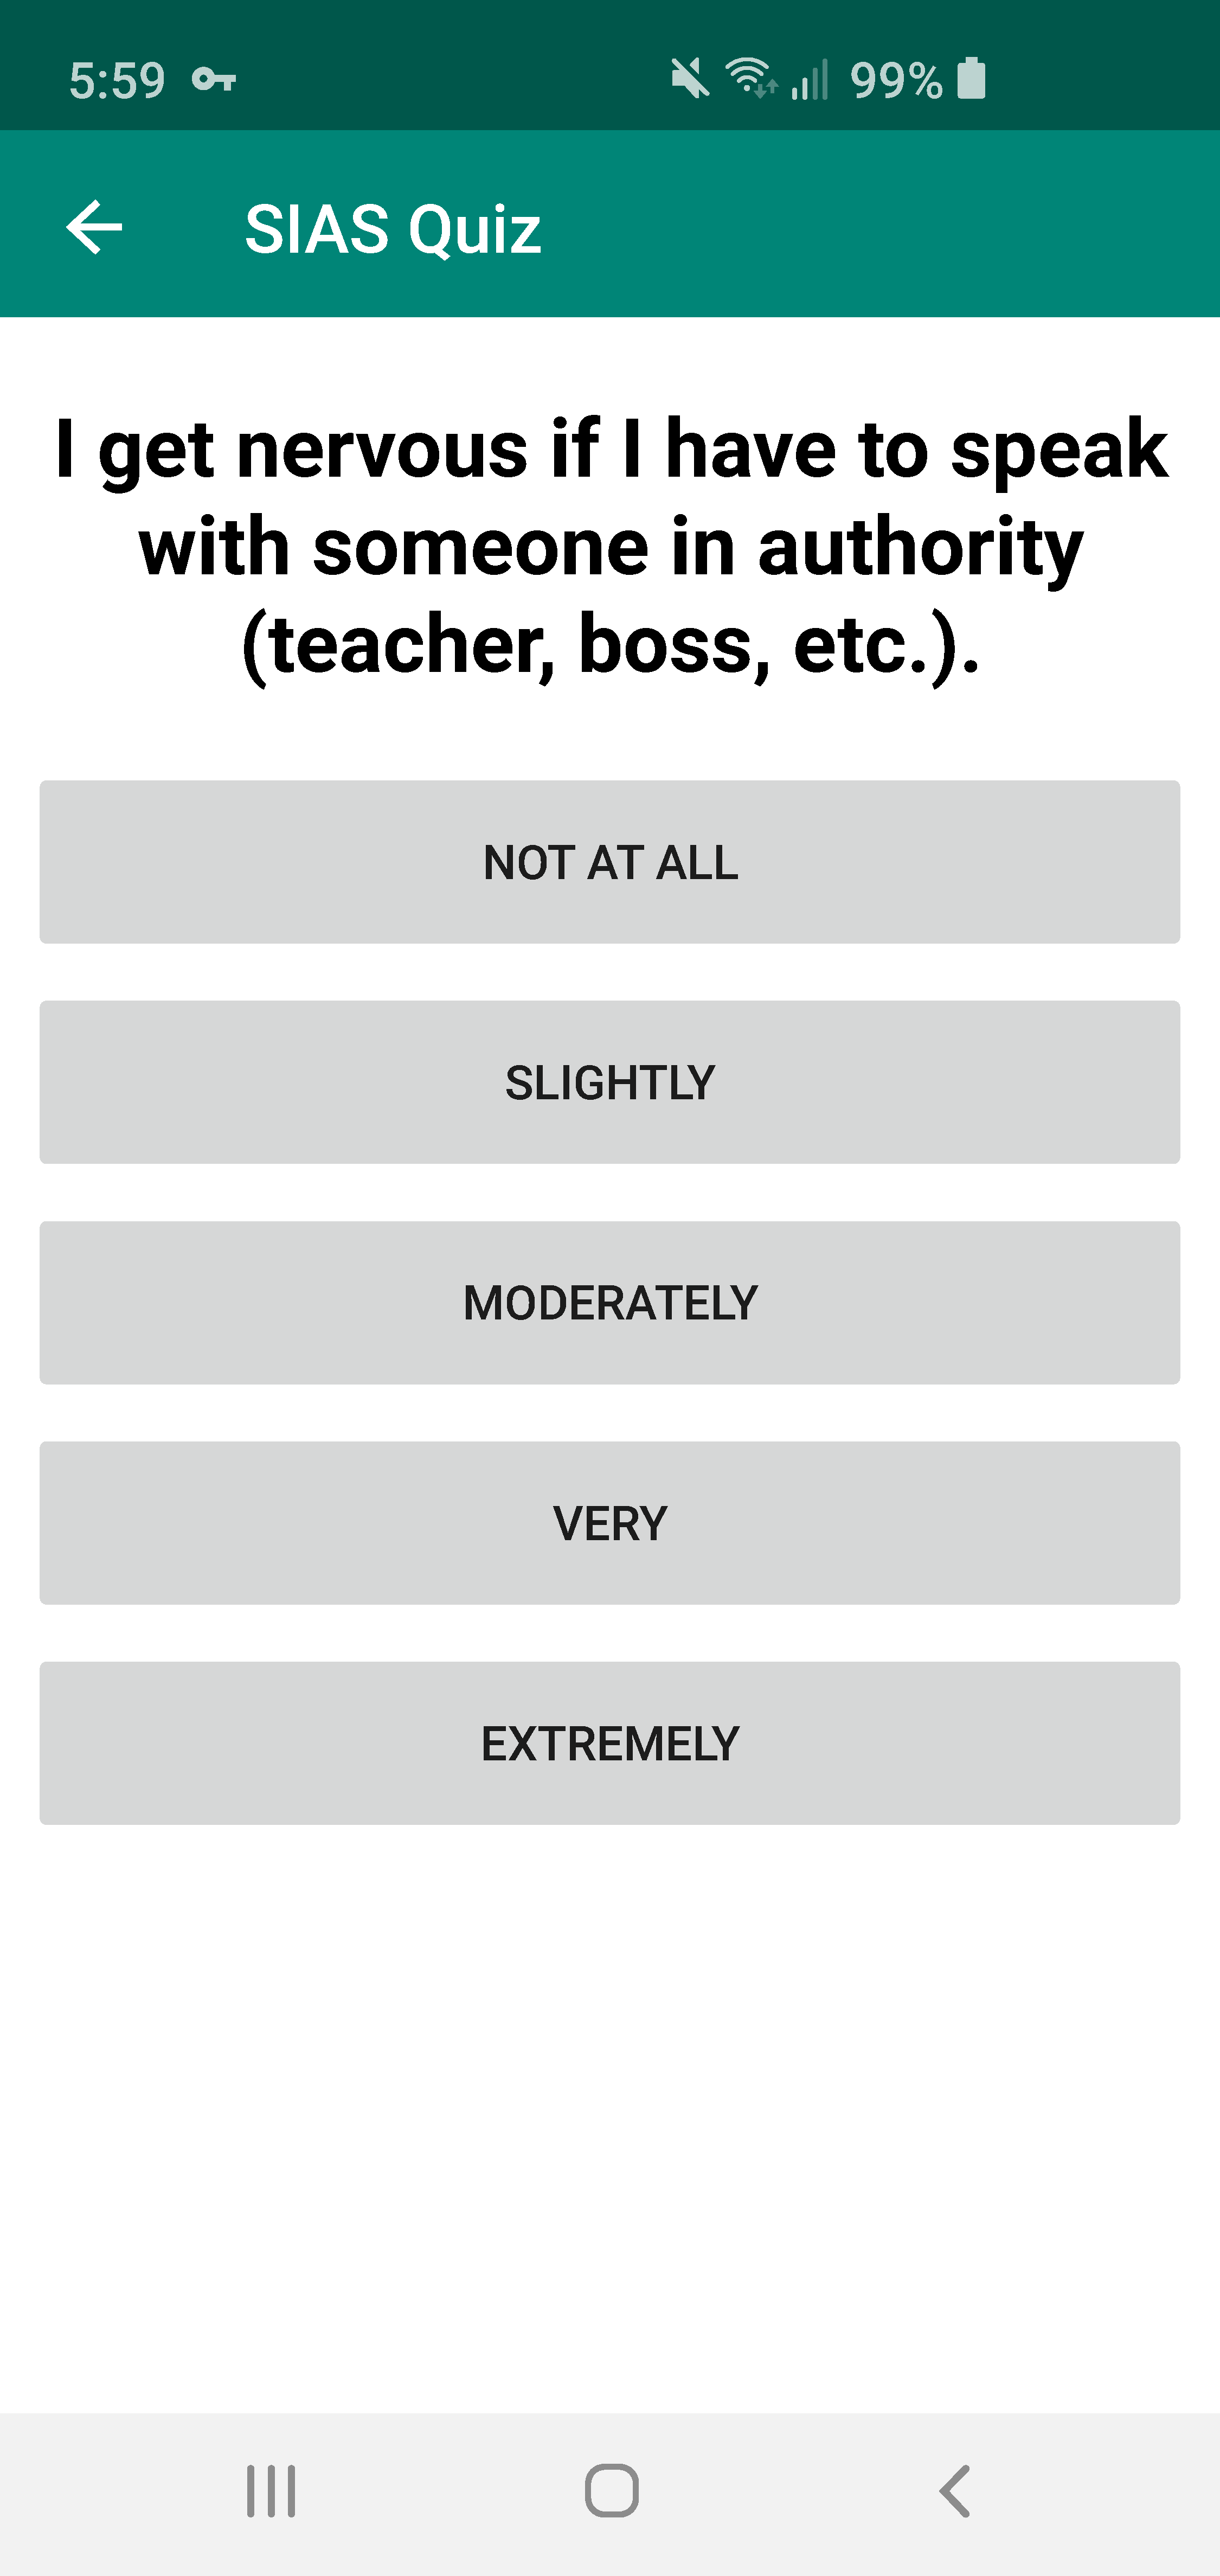
\includegraphics[width=\textwidth]{images/sias.pdf}
        \caption{SIAS Test Question Screen}
        \label{fig:main_screen_1_sias}
    \end{subfigure} \quad
    \begin{subfigure}[b]{0.30\textwidth}
        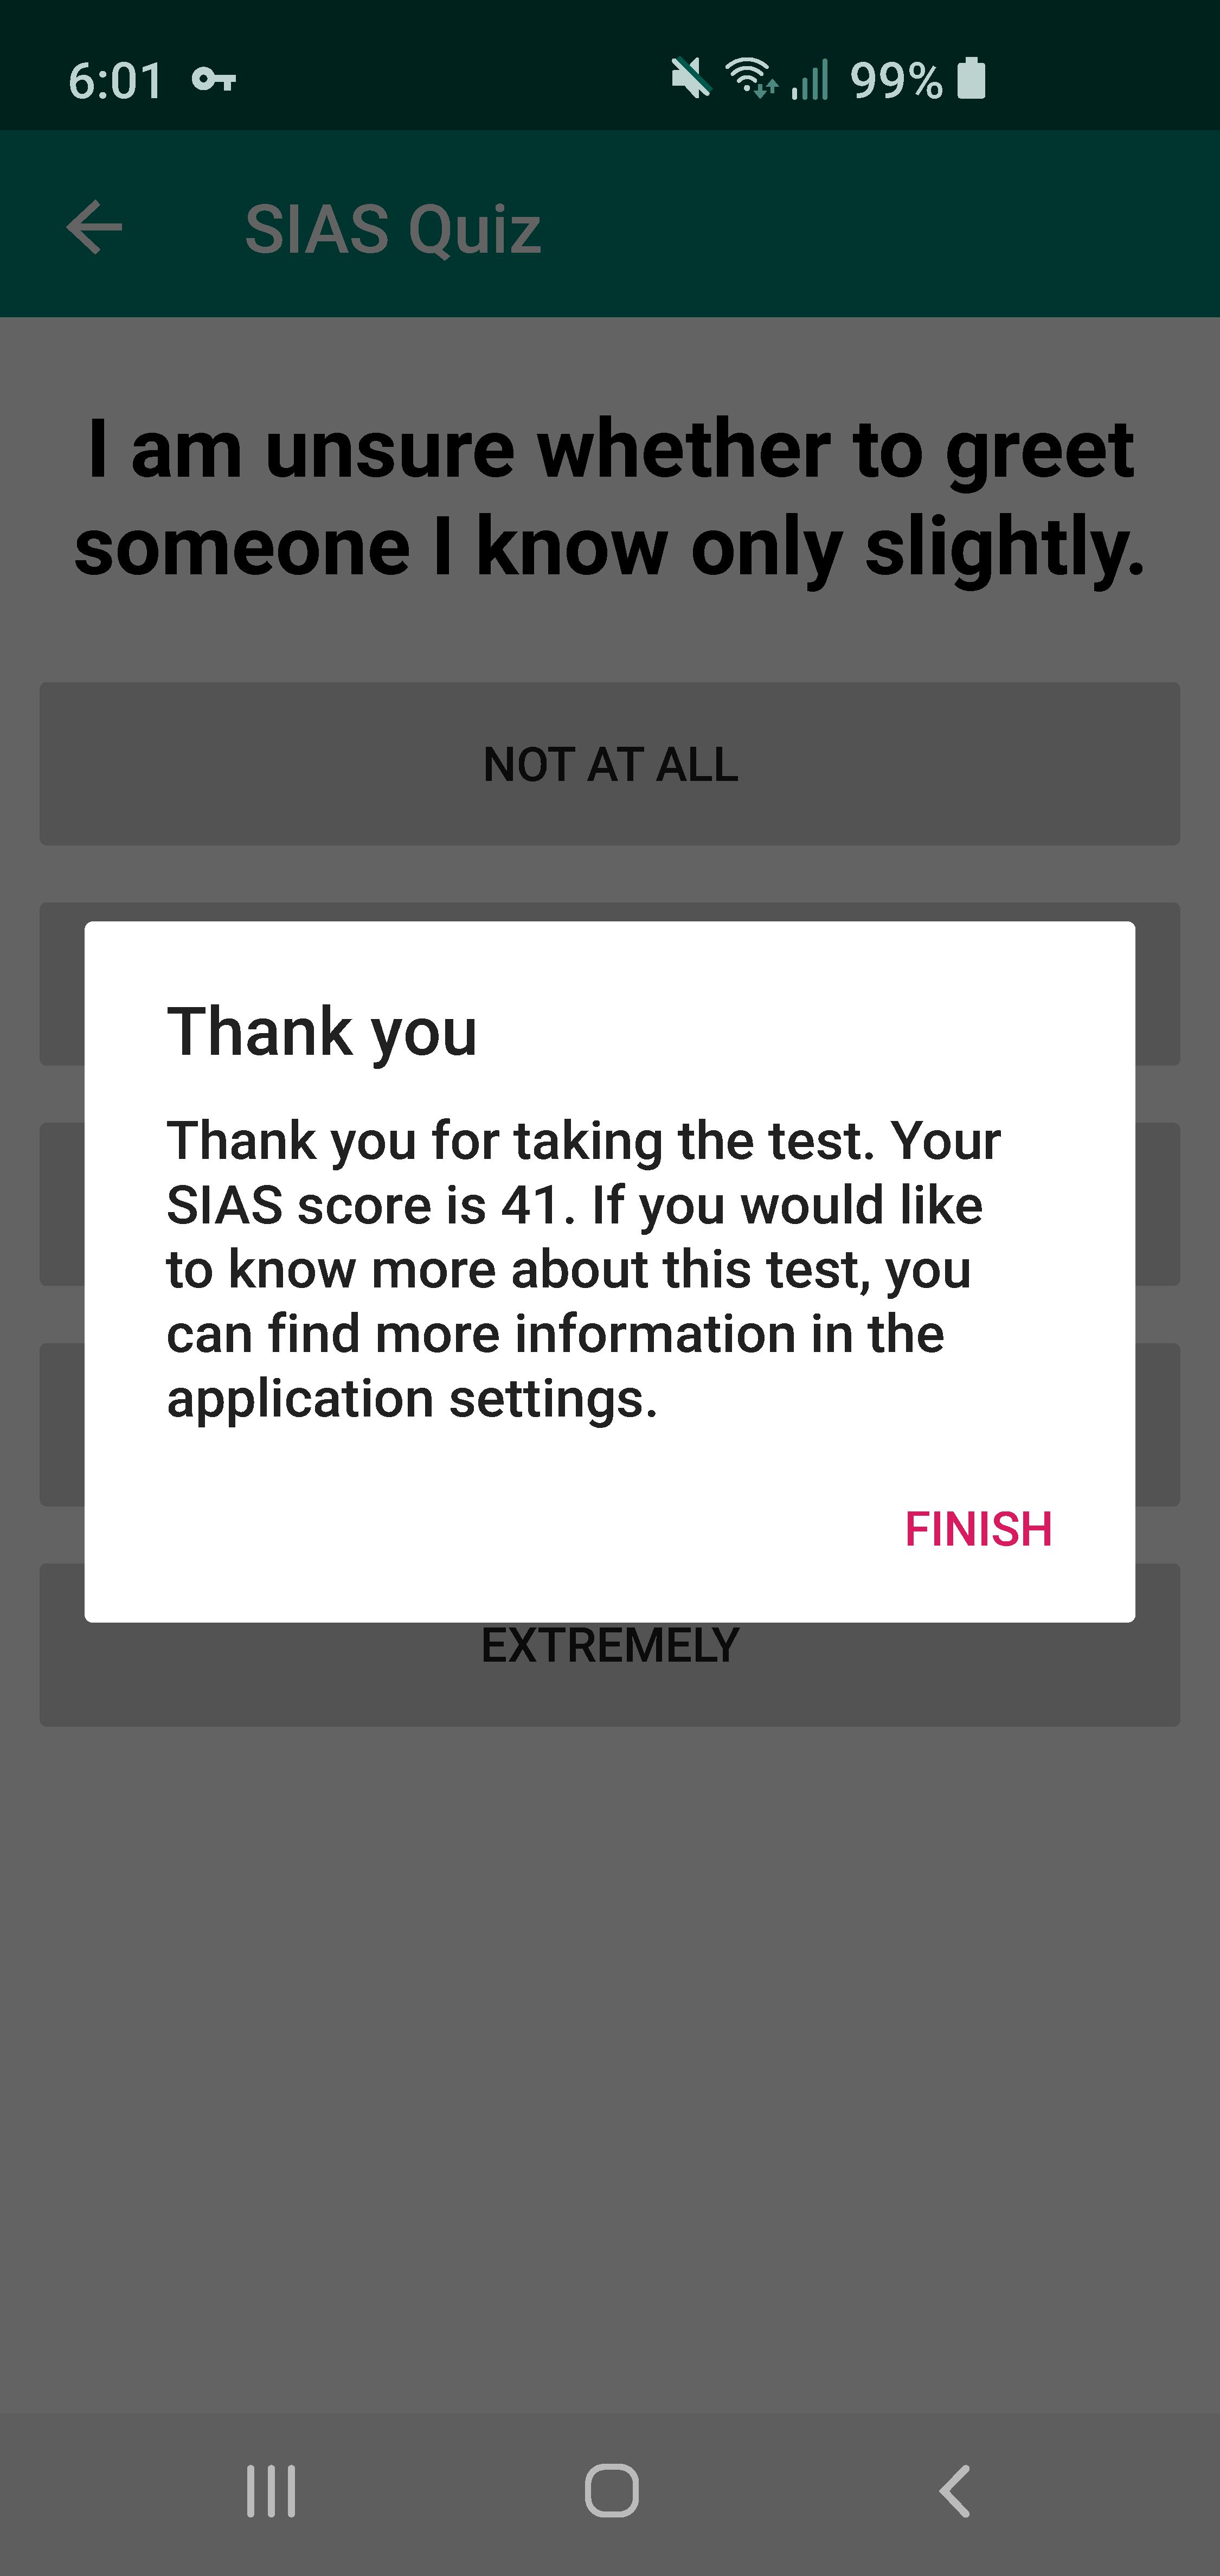
\includegraphics[width=\textwidth]{images/sias-done.pdf}
        \caption{SIAS Test Finish Screen}
        \label{fig:test_screen_1_done}
    \end{subfigure}
    \caption{The implemented SIAS test in Android. The left figure shows how each question will look and the right figure shows the notification that is presented to the participant when they are finished.}\label{fig:sias-android}
\end{figure}

\subsection{Keeping the Application Alive}\label{section:keep-app-alive}
% talk about previous way it was done. talk about android being restrictive. workmanager vs alarmmanager vs this. talk about moving persistent notification to own service for memory
More restrictions on background processing were added to recent Android versions. In Android 6.0, \textit{Doze} and \textit{App Standby}\footnote{\url{https://developer.android.com/training/monitoring-device-state/doze-standby}} were added to further save power. \textit{Doze} defers background CPU activity if the device is unused for a long amount of time. \textit{App Standby} defers background network activity for applications that have not been recently used. Android 8.0 introduced additional background execution limits\footnote{\url{https://developer.android.com/about/versions/oreo/android-8.0-changes}}. These changes required the application to have a visual indicator of some sort whenever it is running in the foreground or background. This way, the user would be informed of what applications are active. Android 9 has more aggressive application standby management as well as applies background execution limits to all applications\footnote{\url{https://developer.android.com/about/versions/pie/power}}.

To account for these changes, the decision to include a persistent notification was made. This would be the visual indicator to the participant to let them know that the application is collecting data. Figure \ref{fig:persistent-notif} shows what the notification looked like. The notification informed the participant that data collection was enabled. This may have led to the participant slightly altering their behaviour knowing that they were being monitored but unfortunately the notification could not be avoided.

Another precaution taken was that the service that keeps the notification shown was to put it in a separate process\footnote{\url{https://developer.android.com/guide/topics/manifest/activity-element.html}}. This would allow it to have its own set of resources and to further try to prohibit the system from removing it. This process would only be responsible for showing the persistent notification, and every other interaction will be on a separate process.

\begin{figure}[htb]
    \centering
    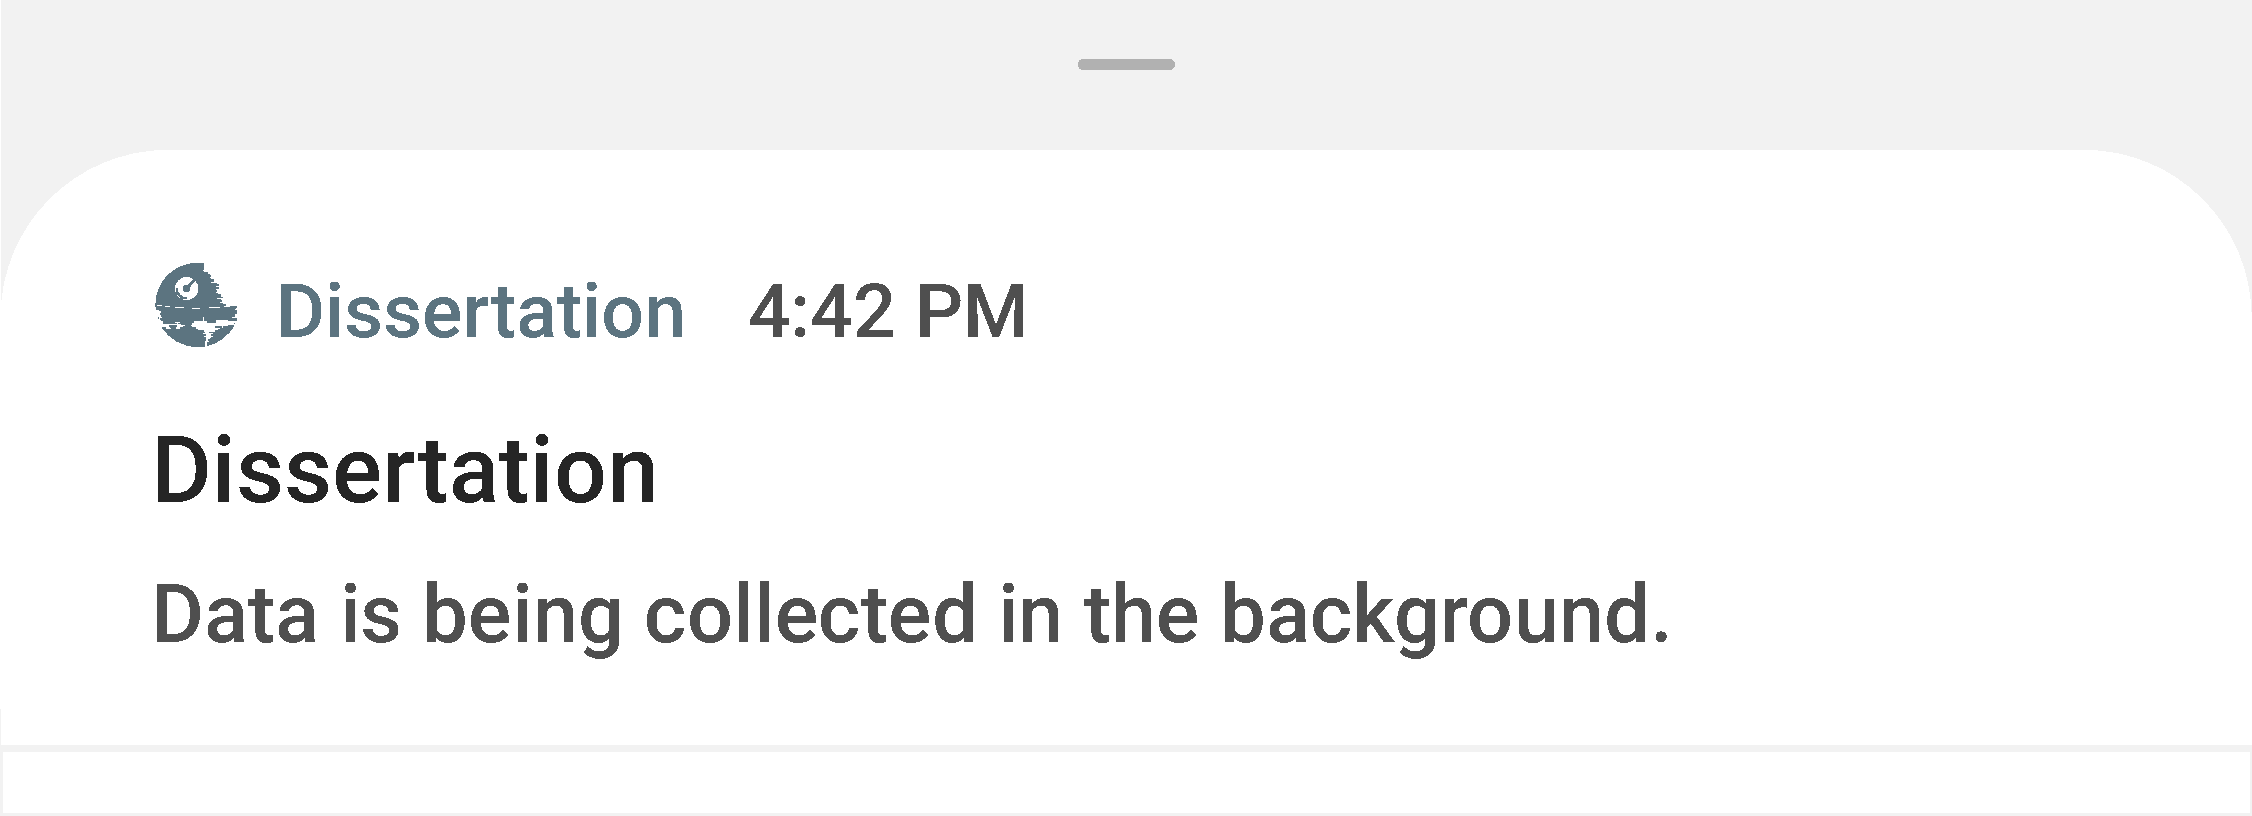
\includegraphics[width=0.80\linewidth]{images/persistent-notif.pdf}    
    \caption{The persistent notification that is shown to the participant. The icon was a vanity choice and only done to differentiate it from other applications. It is an icon of the Death Star from The Noun Project.}
    \label{fig:persistent-notif} 
\end{figure}


\subsection{AWARE Framework}
% talk about aware framework, shortcomings and removing it. maybe mention alternatives caret
The AWARE framework was used in past research (\cite{dimitris}) to gather data in the background. The framework allows for data to be collected from numerous sensors available on the smartphone. It also backs up the data to an external server in a different country. We considered using it but wanted to have full control of where the data was stored\footnote{At the time of decision, we were not aware that the developers were working on \hyperref{https://awareframework.com/aware-light/}{AWARE-Light}. This version of AWARE does not use their servers for backup and instead allows developers to connect it to their own.}. Additionally, we felt like it might add too much overhead and make the application more battery intensive. Implementing the data collection in-house gave us more control in regards to how the data was controlled as well as finer control over battery management.


\subsection{Session Tracking}
A session is defined as the time between device unlock and lock. Android has the ability to broadcast certain system events, including device lock and unlock. Implementing a custom listener to listen to these broadcasts was the initial solution. This solution would run in the background and save each session unlock and lock time. 

Every four hours, a separate service would run and gather actual application data for the collected session times and save to the internal storage. This was implemented by using the native Android Usage Stats Manager API\footnote{\url{https://developer.android.com/reference/android/app/usage/UsageStatsManager}}. This API gathers usage data about applications and can filter by specific time frames. The service was implemented with the Android JobIntentService\footnote{\url{https://developer.android.com/reference/android/support/v4/app/JobIntentService}} API, which handled the background processing. This solution did not rely on a persistent notification running in the background as the Android documentation implied that broadcast listeners that listen to system broadcasts would not be killed.

This initial solution proved to be unstable due to the broadcast listener implementation. The Android system would occasionally stop the broadcast listener service without any notice, and this made it difficult to rely on for data collection. Additionally, as was observed in later iterations, various device manufacturers implement different battery saving\footnote{\url{https://dontkillmyapp.com/}} and process management mechanisms. These custom implementations are not always documented and do not always follow what the Google Android documentation states. The final solution was a third-party open-source library called Dynamic  Engine\footnote{\url{https://github.com/pranavpandey/dynamic-engine}} coupled with the persistent notification mentioned in section \ref{section:keep-app-alive}. It proved to be stable and was straightforward to implement. With this change also came the removal of the background service mentioned previously. Session data was continuously tracked and saved without the need of the four hour period service. This was more reliable and did not negatively impact battery life.


\subsection{Location Gathering}
Location gathering was implemented with the Google Fused Location Provider API\footnote{\url{https://developers.google.com/location-context/fused-location-provider}}. This API combines data from GPS, Wi-Fi, cellular networks, and other phone-based sensors to determine the most accurate location. The API can determine the location on various levels of accuracy, and for this project, the highest accuracy was selected. The interval was set to collect every ten seconds but the system manages this and the interval was not always the same. This is better for battery life as location gathering can scale down if the battery percentage is low.

Previous research (\cite{dimitris, wood}) used the low-level Android location gathering APIs. These require more management and are not able to adapt to battery level or context, as in some situations GPS may not be the most accurate choice. The collection interval should be more stable  since the system is not managing it. This was determined to be a necessary trade-off as accuracy was hypothesised to be more beneficial overall compared to a stable interval. There is additionally the issue of GPS drift. According to \cite{maps_youtube}, the Fused API is implemented to take GPS drift into account as well as provide more quality location data. 

\subsection{Call Tracking}
Call duration tracking was implemented with Dynamic Engine. The start and end times of each call are recorded and saved to internal storage. The recipient is unknown as is the content of the call, as the microphone was not monitored.\footnote{We would like to note that even though call data was collected, we did not have time to integrate it with the other data and use it to compare with past research. We mention it here for historical purpose.}


\subsection{Data Export}
Data export was implemented by sending all the data from the device to a cloud server that would then save it to a database. This would be done through network calls. Android provides standard networking capabilities through the library Volley\footnote{\url{https://developer.android.com/training/volley}}. Volley would be more than enough for the project scope but the choice was made to go with a different third party network library. OkHttp\footnote{\url{https://square.github.io/okhttp/}} was chosen for its straightforward API.

Data export works by sending all of the data serialised as JSON through post requests. This is a standard method of transportation and ensured that data integrity would persist.

Initially data export was to be implemented as an export to a comma-separated value (CSV) file that would then be sent to us. This would remove the anonymity of the participant completely and may result in less overall participants in the study. Hence the decision was made to automate the data export. It is important to note that there is still an option to export the data as a CSV file but it is not sent to the researcher.

\subsection{Battery Consumption}
Battery consumption was a major concern from the first iteration. To achieve a desirable result, native system APIs were used as much as possible. This would allow Android to optimise internally. The location and session gathering were determined to be the most intensive services. The location gatherer was tested with various interval sizes, and it was observed that aggressive intervals did not have a high negligible impact on battery consumption. The session gatherer ran in the background and was controlled by the system. This allowed Android to run it when the condition was favourable and thus could avoid impacting battery life.

\subsection{Application Crash Tracking}
The application had a crash tracking service integrated. This allowed us to see unknown bugs that may appear during testing on multiple devices. Three solutions were researched, Bugsnag\footnote{\url{https://www.bugsnag.com/}}, Sentry\footnote{\url{https://sentry.io/welcome/}}, and Firebase Crashlytics\footnote{\url{https://firebase.google.com/products/crashlytics}}. All three offer an extensive free plan that would be enough for the project. All three can be extended so that custom errors can be logged. We had experience with all three and chose to use Sentry because it had a simple integration process. Using this service came from the non-functional requirement \textbf{27}.

\subsection{Application Memory Leak Tracking}
The application used LeakCanary\footnote{\url{https://square.github.io/leakcanary/}} during development to track any memory leaks that may occur. This comes from requirement \textbf{23}. Eliminating memory leaks is a key component of reducing battery consumption and ensuring that the user experience is smooth.

\subsection{Settings Options}
A brief look at the settings options available to the participant will be discussed.

\begin{itemize}
    \item Export to CSV - The option to export to a local CSV file was added. This was part of non-functional requirement \textbf{22}. OpenCSV\footnote{\url{http://opencsv.sourceforge.net/}} was used to implement this option.
    \item View identifier and SIAS score - This was part of non-functional requirement \textbf{22}. It was added to provide more transparency.
    \item Permissions - Each required permission was implemented as a separate toggle button that would indicate if the permission was enabled or not.
    \item Opt-out - This was implemented as an external link to a Google Form. The form asked for the identifier. This allowed a participant to opt-out anonymously, and if their data was already sent, the identifier could be used to remove it from the database. This was requirement \textbf{10}.
    \item Learning more - This was implemented as an external link to a page on the Github wiki that gave some more detail about the project as well as the SIAS exam itself. This was requirement \textbf{26}.
\end{itemize}


\section{Server and Database}\label{section:server-db-impl}
This section will discuss the implementation of the server and database systems.

\subsection{Server}
The server had the job of receiving, processing, and sending the data to the database. It could either be local or remote. Maintaining a remote server is an easier task, and so it was decided to use a remote server on the cloud. Amazon Web Services\footnote{\url{https://aws.amazon.com/}} (AWS) was chosen for this, specifically their Elastic Compute Cloud service\footnote{\url{https://aws.amazon.com/ec2/}}. Google Cloud Platform\footnote{\url{https://cloud.google.com/}} and Microsoft Azure\footnote{\url{https://azure.microsoft.com/en-us/}} were considered but Amazon Web Services is considered the most mature of the three services.

The server ran Ubuntu 18.04\footnote{\url{https://ubuntu.com/}}.  Nginx\footnote{\url{https://nginx.org/}} was set up to listen to incoming requests. It would receive requests and proxy them to the relevant port on the machine. This is the Receiver in Figure \ref{fig:server_diagram}. To keep connections encrypted, Let's Encrypt\footnote{\url{https://letsencrypt.org/}} was used to create a TLS certificate. A virtual private cloud on AWS was created. Permission access was set to allow incoming HTTP and HTTPS from everywhere and SSH connection only from us. This setup would meet requirements \textbf{19}, \textbf{20}, \textbf{30}, and \textbf{31}.

Three server-side languages were considered for the implementation of the Processor from Figure \ref{fig:server_diagram}. The first one was Node.js and either the Express\footnote{\url{https://expressjs.com/}} or Fastify\footnote{\url{https://www.fastify.io/}} HTTP framework. The second choice was Python and Flask\footnote{\url{https://palletsprojects.com/p/flask/}}, and the third choice was PHP and Laravel Lumen\footnote{\url{https://lumen.laravel.com/}}. All three frameworks are resilient and can be used to make an API service quickly. There is small to no overhead, and they are extensible as well as popular. All three of them would meet requirement \textbf{29}. Node.js was chosen alongside Fastify to implement the data Processor. Fastify checked each request to see if it contained the allowed secret key, which would mean that the request has come from a participant device. This met requirement \textbf{21}. The object-relational mapping (ORM) tool Sequelize\footnote{\url{https://sequelize.org/}} was chosen to convert and save the data from each request to the database. The connection to the database used the AWS root certificate to enable SSL.

\subsection{Database}
The Android database layer Room uses SQLite in the background and hence made sense to model the remote database as close as possible to it. This would allow for quicker data transition and less time spent in processing. MariaDB was chosen for the database engine. It is SQL compliant and widely supported. The database was set up with the AWS relational database service\footnote{\url{https://aws.amazon.com/rds/}} (RDS) tool. It was in the same VPC as the network but with the difference that it was visible only to services within the network as well as us. This met requirement \textbf{30}. The database was set up to encrypt the data at rest, meeting requirement \textbf{19}.

\section{Data Analysis}
For data analysis, the programming language Python 3\footnote{\url{https://www.python.org/}} was used. R\footnote{\url{https://www.r-project.org/about.html}} was considered but we have more experience with Python. Python has a wide variety of data analysis and machine learning libraries, and is widely supported. For the data pre-processing, we chose to use the NumPy\footnote{\url{https://numpy.org/}} and Pandas\footnote{\url{https://pandas.pydata.org/}} packages. These are both widely used, tested, and stable for our purposes. These libraries can be used to sanitise and clean the data, meeting requirement \textbf{13}. Pandas is able to produce a variety of statistical information.

\subsection{Training Classifiers}
Scikit-learn (\cite{scikit-learn, sklearn_api}) was used for classifier training. Sci-kit learn has an assortment of machine learning classifiers as well as other data processing tools. We considered XGBoost\footnote{\url{https://xgboost.readthedocs.io/en/latest/}} but XGBoost does not have a decision tree classifier. Additionally, the past projects by \cite{dimitris, wood, fox} used scikit-learn, and so it would be more straightforward to compare our results with theirs when using the same library. Scikit-learn was used to meet requirement \textbf{14}, \textbf{15}, and \textbf{16}.

\subsection{Generating Graphs and Charts}
Matplotlib\footnote{\url{https://matplotlib.org/}} and Seaborn\footnote{\url{https://seaborn.pydata.org/}} were used to create graphs and charts. These are widely supported libraries and have thorough documentation. We used the Google Maps Geocoding API\footnote{\url{https://developers.google.com/maps/documentation/geocoding/start}} to extract location categories from latitude and longitude coordinates. The data analysis was implemented in a Jupyter\footnote{\url{https://jupyter.org/}} notebook.


\section{Summary}
This chapter looked at how the various project parts were implemented and why certain technologies were chosen. Each section of this chapter shows the specific requirements that were met. We described in detail the implementation of the various application systems. Then we looked at the implementation of the server and database, and how they fulfil their roles as data receiver and store respectively. Finally, we looked at the technologies used for the data analysis. 

%==================================================================================================================================
\chapter{Evaluation} \label{evaluation}
% setup siunitx to have two decimal places
\sisetup{
	round-mode = places,
	round-precision = 2
}
This chapter will discuss the results of the project and look at various shortcomings. First, the user study will be briefly described. Next, various classifier model performances with location and application usage data will be shown. Finally, there will be a short discussion about the evaluation of the application during the user study.

\section{User Study Procedure}
The user study consisted of two trials. The first one had 18 participants. The participants were recruited and shown the introduction script in Appendix Figure \ref{fig:intro_script}. After their consent was recorded by the form in Appendix Figure \ref{fig:consent_form}, they were asked to install the application, take the SIAS quiz, and enable data collection. This trial ran for a week. After it finished, the participants were debriefed with the script in Appendix Figure \ref{fig:debrief_script} and given a short survey, shown in Appendix Figures \ref{fig:device_form1}, \ref{fig:device_form2}, and \ref{fig:device_form3}, to fill out. The first trial exposed an error in how location data was gathered, and so a second trial was repeated with a new fixed version of the application. The collected data from the first trial was invalidated but the responses from the survey were kept. The second trial had 16 participants, as two had to opt-out due to device issues unrelated to the application. The collected data from trial two was used throughout the evaluation.

\section{Application}
The application and its interface was not thoroughly evaluated as it was not the main focus. Basic statistics were gathered from the survey to see how it performed and how participants felt during the study. 14 participants filled in the survey. A majority of participants felt comfortable about having their location tracked, as shown in Appendix Figure \ref{fig:location_tracking_comfort}. This matches the result of \cite{wood}. A significant portion of participants felt comfortable knowing their data was being analysed, as shown in Appendix Figure \ref{fig:data_analysis_comfort}. An overwhelming amount of participants stated that they did not change or think about changing their behaviour since their usage data was being gathered. This is beneficial because it shows that there is very little bias in the data gathered due to purposefully altered behaviour. A large majority of participants felt comfortable knowing that their usage data was readily available, as shown in Appendix Figure \ref{fig:usage_stats}. 

Participants reported favourable battery drainage throughout both trials. From the survey, a majority reported that the application used about 0.5\% of battery every three hours. Some reported even lower statistics but we assume that this may be because they may have disabled location and that part of the application was not active. In one extreme case, the location gathering actually used around 15\% of battery every three hours, and the participant had to disable it every once in a while. 

Participants had a large spread of RAM usage. Usage spanned from 10 megabytes to over 150 megabytes, with no noticeable pattern. We suspect this large variance comes from the different battery saver mechanisms that each device implements. Participants reported application closure on devices that had 1 gigabyte of RAM.

\section{Location Data}
\subsection{Method}
The location data was separated into rows. Each SIAS score was mapped to either 0 or 1, with the former meaning that the individual has a score below 34 and the latter meaning that the individual has a score of or above 34. This threshold value results in a binary classification problem and is also the value used by \cite{wood, boukhechba} in their projects. The average of the SIAS scores in the data is \num{0.1506}. This shows that there is a notable difference between the location data  rows that belong to socially anxious individuals compared to those that are not socially anxious, with the former being lower. The standard deviation is \num{0.3577} and the variance is \num{0.1279}. Figure \ref{fig:location_sias_scores_distribution} shows the distribution in the rows that belong to users with a SIAS score below 34 (0) and above 34 (1).

\begin{figure}[htb]
    \centering
    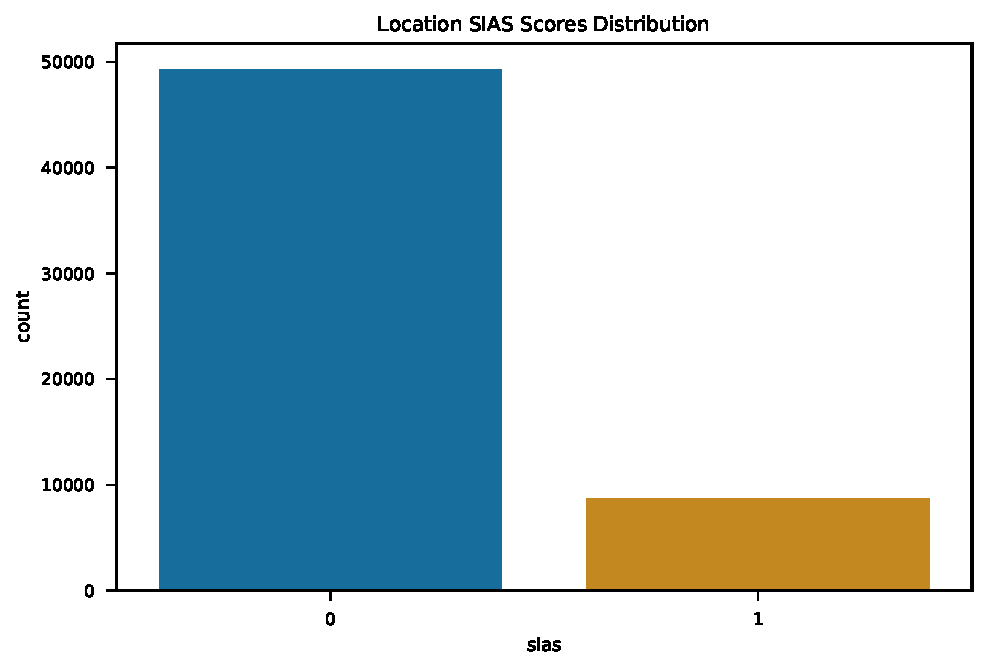
\includegraphics[width=0.85\linewidth]{images/location/bar_chart_Location_SIAS_Scores_Distribution.pdf}
    \caption{This figure shows the imbalance between the amount of data between users with a SIAS score of below 34, grouped as 0 above, and score of and above 34, grouped as 1 above.}
    \label{fig:location_sias_scores_distribution} 
\end{figure}

Each latitude and longitude coordinate pair was mapped to a location category based on the Places Reverse Geocoder API. There were 31 categories identified, with Figure \ref{fig:location_category_distribution} showing the distribution. These were the extracted features. It can be seen that there is an imbalance of categories, with category \textit{point\_of\_interest} at 68\% followed by \textit{home} at 18\%. Figure \ref{fig:location_category_correlations} shows the Pearson\footnote{\url{http://learntech.uwe.ac.uk/da/Default.aspx?pageid=1442}} correlations between the categories and SIAS score. It can be observed that a majority of the correlations are weak or negative, with the exception of category \textit{home} having an overall stronger positive correlation to the SIAS score.

\begin{figure}[htb]
    \centering
    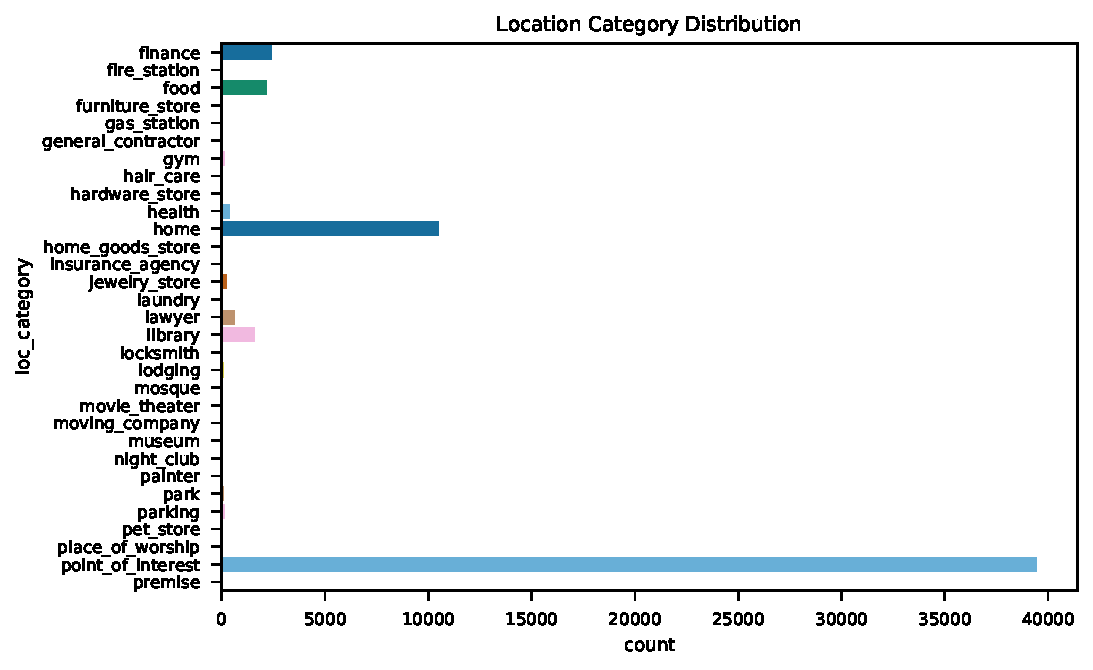
\includegraphics[width=\linewidth]{images/location/bar_chart_Location_Category_Distribution.pdf}
    \caption{This figure shows the distribution in category labels in the data set. \textit{point\_of\_interest} makes up 68\% of the data. 96\% of the distribution is shared between six categories.}
    \label{fig:location_category_distribution} 
\end{figure}


\interfootnotelinepenalty=10000
\subsection{Classifier Performance}
A decision tree classifier was used to create a model to see if location data alone could be an accurate identifier of social anxiety. The tree used the Gini impurity measure\footnote{We considered the entropy measure for information gain but it has been shown that the two measures produce similar results with a very small percentage difference \citep{gini_vs_entropy}. During testing with location data, no noticeable difference was seen and so we went with the Gini impurity.} and had no set maximum depth. The model was initially trained without up-sampling of the data to try to account for the imbalance. There was an 80\%/20\% split for training and testing data. The metrics for this model can be seen in table \ref{table:location_no_upsampling_metrics}. The f1 score for predicting no social anxiety is high but because of the class imbalance, the f1 score for predicting social anxiety is much lower. The confusion matrix in Figure \ref{fig:location_no_upsampling_matrix} shows that the model did confuse a socially anxious individual with a non-socially anxious one. Figure \ref{fig:location_no_upsampling_importance} shows the feature importance, with the \textit{home} category considered the most important. This ties in with the positive correlation that can be seen in Figure \ref{fig:location_category_correlations}. The model was cross-validated with a stratified KFold\footnote{\url{https://scikit-learn.org/stable/modules/generated/sklearn.model_selection.StratifiedKFold.html}} strategy with 30 folds. Figure \ref{fig:location_no_upsampling_kfold} shows how the model performed with cross-validation. This was done to try to avoid overfitting and provide further validity to the model.

\begin{table}[htb]
\centering
\begin{tabular}{@{}cccc@{}}
 & \textbf{Precision} & \textbf{Recall} & \textbf{F1} \\ \midrule
\textbf{0} & 0.90 & 0.94 & 0.92 \\
\textbf{1} & 0.65 & 0.54 & 0.59
\end{tabular}
\caption{This table shows the metrics for the decision tree classifier without up-sampling the location data. It can be seen that the f1 score is high for 0 (no anxiety) but significantly lower for 1 (social anxiety). This can be attributed to the large class imbalance that is present. The classifier model here had an overall accuracy of 86\%.}
\label{table:location_no_upsampling_metrics}
\end{table}

\begin{figure}[htb]
    \centering
    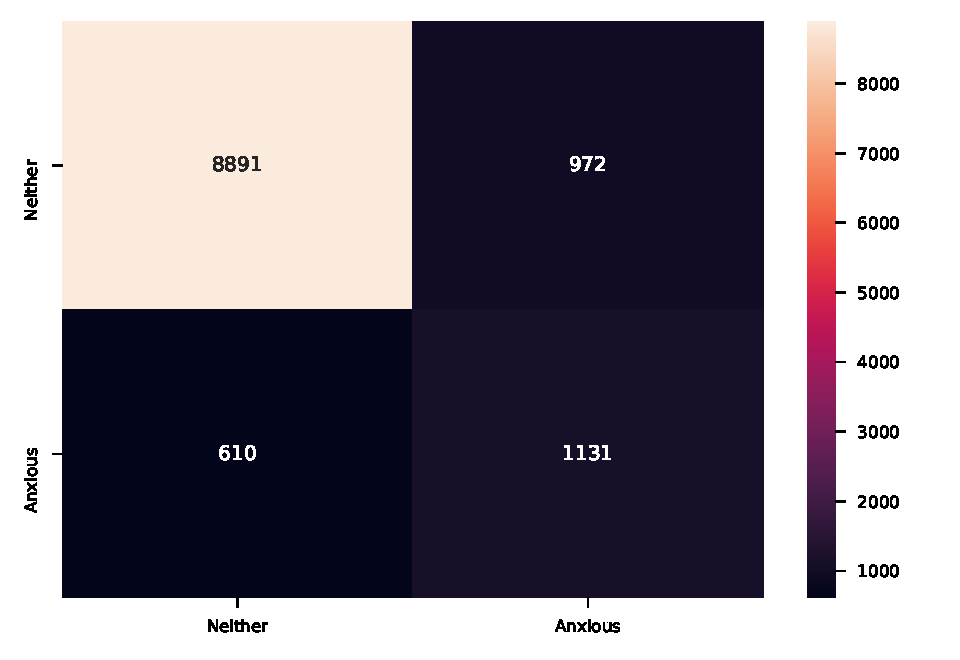
\includegraphics[width=0.75\linewidth]{images/location/heatmap_Decision_Tree_Locations.pdf}
    \caption{This figure shows the confusion matrix for the classifier without up-sampling the location data. The classifier is not accurate across all classes because of the class imbalance.}
    \label{fig:location_no_upsampling_matrix} 
\end{figure}

\begin{figure}[htb]
    \centering
    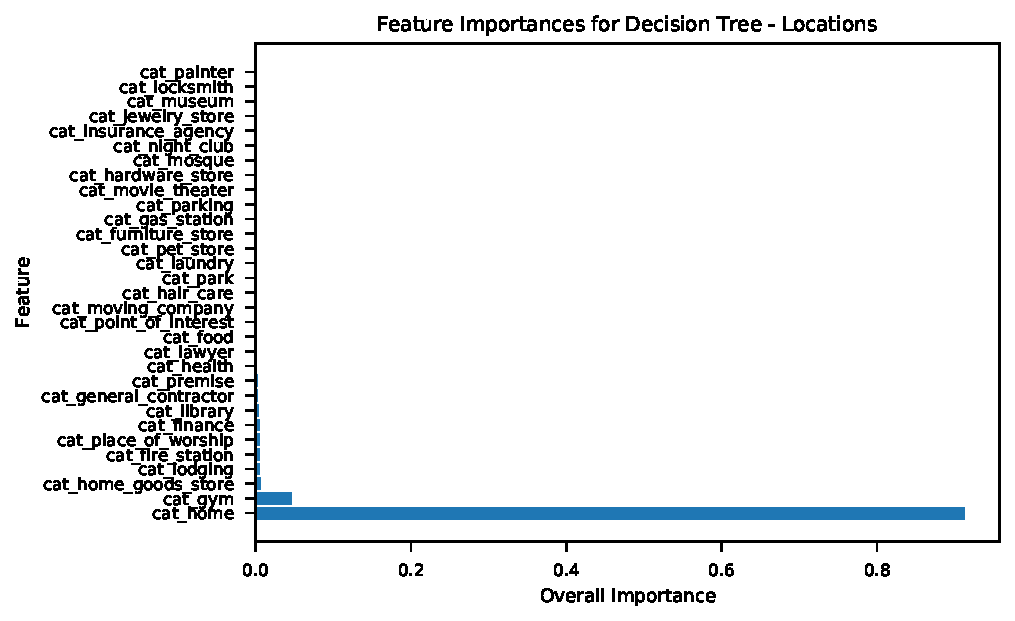
\includegraphics[width=0.95\linewidth]{images/location/feature_importance_DecisionTreeLocations.pdf}
    \caption{This figure shows the feature importance for the decision tree classifier trained with the location data. It can be seen that category \textit{home} has the highest importance, which corresponds with its higher correlation as seen in Figure \ref{fig:location_category_correlations}.}
    \label{fig:location_no_upsampling_importance} 
\end{figure}


A second model was trained with up-sampled data. The minority classes were up-sampled using SMOTE (\cite{smote}) from the imbalanced-learn\footnote{\url{https://imbalanced-learn.readthedocs.io/en/stable/index.html}} package. This was done to try to reduce the effects of the class imbalance. Table \ref{table:location_sm_metrics} shows the scores for this classifier. It can be seen that there is not much of a difference and it suggests that class imbalance may not be the only problem. There may be an overfitting or under-fitting due to a specific feature instead of a lack of data. This model was cross-validated with a stratified KFold strategy with 30 folds. Figures \ref{fig:location_sm_matrix}, \ref{fig:location_sm_feature_importance}, \ref{fig:location_sm_kfold} in the Appendix show the confusion matrix, feature importance, and cross-validation results of the up-sampled model. The figures further suggest that the model may be affected by other factors besides class imbalance.

\begin{table}[htb]
\centering
\begin{tabular}{@{}cccc@{}}
 & \textbf{Precision} & \textbf{Recall} & \textbf{F1} \\ \midrule
\textbf{0} & 0.89 & 0.94 & 0.91 \\
\textbf{1} & 0.65 & 0.52 & 0.58
\end{tabular}
\caption{This table shows the metrics for the decision tree classifier with up-sampling of the location data. It can be seen that there is very little difference in the scores, and is not enough to conclude that the class imbalance is the main reason for the lower f1 score in predicting social anxiety.}
\label{table:location_sm_metrics}
\end{table}

\subsection{Previous Experiments}
The strong correlation above between the \textit{home} category and the SIAS score suggests that social anxiety may be more prevalent in individuals that stay home more often, which matches similar conclusions achieved by \cite{wood, mobile_sensing_for_depression_social_anxiety, boukhechba}. The current classifier model differs from \cite{wood} in that they ran their study for a day and this one ran for a week. The accuracy of the model closes matches that of what \cite{boukhechba} achieved with location data alone. All three studies used current university students as participants. We were not able to integrate call data with location data to be able to see how mobility and communication patterns perform. This would have allowed for a more thorough comparison with \cite{boukhechba}.


\subsection{Issues and Discussion}
The location data that was collected was not complete because not every participant agreed to send location data. In some situations, even when they agreed, if their location was disabled then the application would not receive updates. It was expected that not every participant would agree to their location data being collected but it was not expected that the device would not receive updates if the location was turned off. This could be attributed to the Fused Location provider API only sending updates if the location was turned on. This method of location data collected differed from \cite{wood} because they did not use this specific API but instead got the raw values from the device. It could also be attributed to battery saving measures taken by the device and thus out of our control. These location data inaccuracies could not be fully fixed in the given time-frame.

In some cases, the location category could be inaccurate. The Google Maps Places API returned multiple addresses per coordinate pair and the exact location and location type had to be inferred from the results. Additionally, as mentioned by \cite{wood}, some locations may be above others, for example, a home may be above a restaurant, and so the API would return the category for the restaurant instead.

The classifier suffers from a lack of features. Specifically, the category feature could be considered one unique feature. Latitude and longitude numbers could not be used directly as they are floating-point and would be subject to large floating-point errors. Some data points could not be considered as features, such as timestamps, location bearing, and accuracy. Some of these measures, like accuracy, are only available on newer Android version, and not every participant had a phone with a compatible version. We felt like using accuracy in conjunction with bearing data could provide more reliable results, because it could be used to filter out locations that may be inaccurate or incorrect. Additionally, the change of direction of the participant could be extracted as a feature and observed.

Overall it can be concluded that location is a good indicator of an individual's social anxiety level. We feel that more research should be done with location to see what features are most effective. Special care should be taken when gathering and processing the data because many factors can taint it and reduce its quality. As \cite{wood, boukhechba} found, an individual who is at home more often may be more socially anxious. At home, they may feel safer and would not be exposed to any socially intense situations. The study should be repeated with more participants as well as with more consistent location data collection. Our model was not entirely accurate due to the lack of features but we think it provides further argument for using location data as an estimator of social anxiety.


\section{Application Session Data}
\subsection{Method}
The application session data was split into rows, with each row representing an individual application from a session. Scores were mapped to either 0 or 1, with the former meaning that the individual has a score below 34 and the former meaning that the individual has a score of or above 34. This threshold value results in a binary classification problem and is also the value used by \cite{wood, boukhechba} in their projects. The average of the SIAS scores in the rows is \num{0.40}. This shows that there is a small class imbalance between socially anxious and non-socially anxious people. The standard deviation is \num{0.49} and the variance is \num{0.24}. Figure \ref{fig:session_sias_distribution} shows the score distribution among the session data rows.

\begin{figure}[htb]
    \centering
    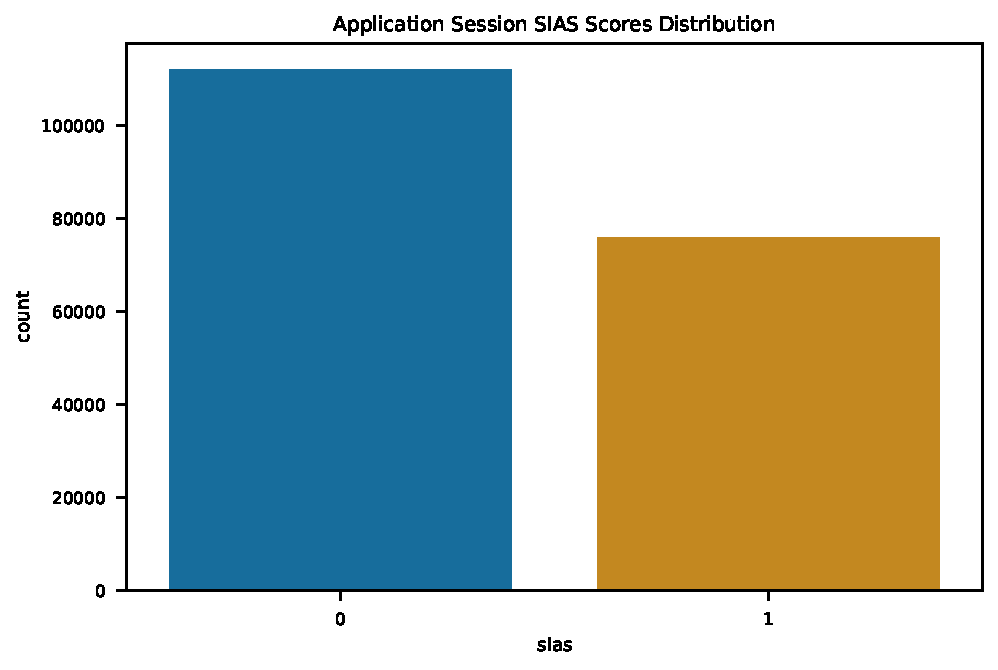
\includegraphics[width=0.65\linewidth]{images/sessions/bar_chart_ApplicationSessionSIASScoresDistribution.pdf}
    \caption{This figure shows the distribution of scores. \num{60}\% of the data was labelled as not socially anxious, and \num{40}\% as socially anxious. This is a small class imbalance.}
    \label{fig:session_sias_distribution} 
\end{figure}

The features that were extracted from the session data was \textit{totalTimeInForeground} and \textit{sessionLength}. \textit{totalTimeInForeground} represents the time that the application spent in the foreground. The foreground is when it is visible to the user and usually meant that they were interacting with it. \textit{sessionLength} is how long the overall session that contained the respective application is. Figure \ref{fig:session_feature_correlation} shows the correlation between the features and the SIAS score. It can be seen that there is not a strong correlation between the features and the SIAS scores. Figure \ref{fig:session_app_categories} shows the categories of applications that were present. The most popular one is \textit{Social \& Communication} at \num{34}\% followed by \textit{Productivity} at \num{21}\%. Figure \ref{fig:categories_among_non_anxious} shows the application category distribution for non-anxious users specifically. Figure \ref{fig:categories_among_anxious} shows the application category for socially-anxious users. It is important to note that almost every application that comes with the system, for example Bluetooth and WiFi Settings, did not have a category assigned to it. These applications were manually assigned the category \textit{System}. These applications were filtered out during the data analysis because they are applications that either came pre-installed or were not directly ran by the individual.

\begin{figure}[htb]
    \centering
    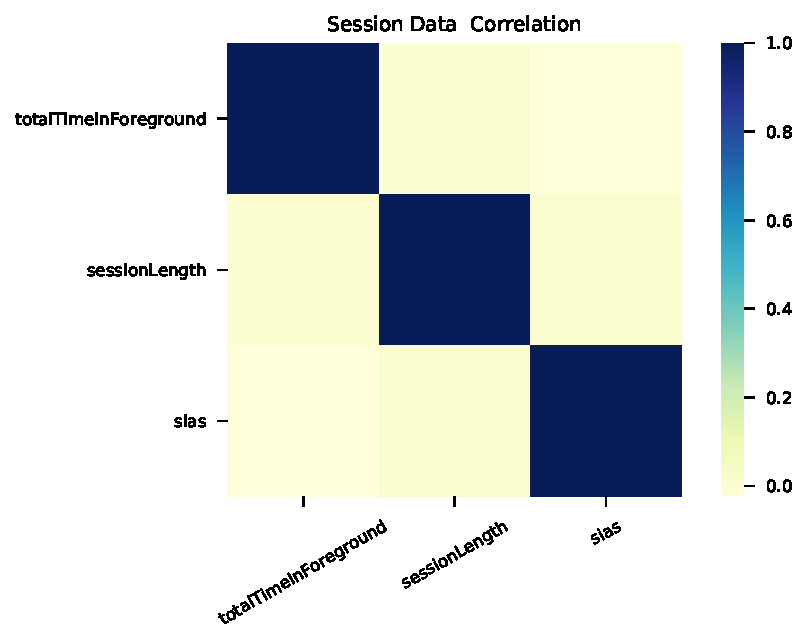
\includegraphics[width=0.75\linewidth]{images/sessions/correlation_SessionData.pdf}
    \caption{This figure shows the correlation between the application session usage data features and the SIAS score.}
    \label{fig:session_feature_correlation} 
\end{figure}

\begin{figure}[htb]
    \centering
    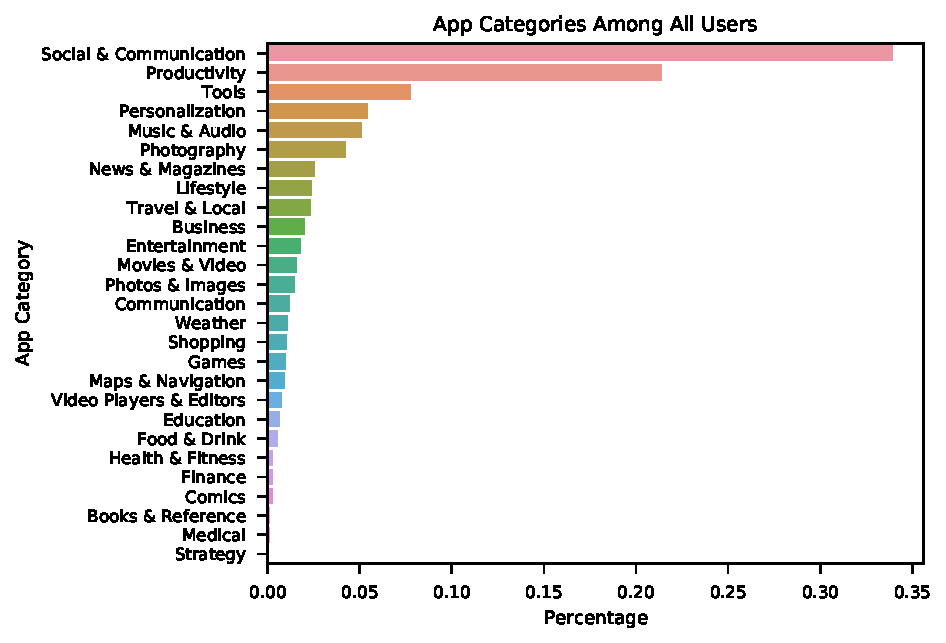
\includegraphics[width=\linewidth]{images/sessions/bar_chart_ApplicationSessionCategoryDistribution.pdf}
    \caption{This figure shows the distribution in application categories in all users.}
    \label{fig:session_app_categories} 
\end{figure}

\begin{figure}[htb]
    \centering
    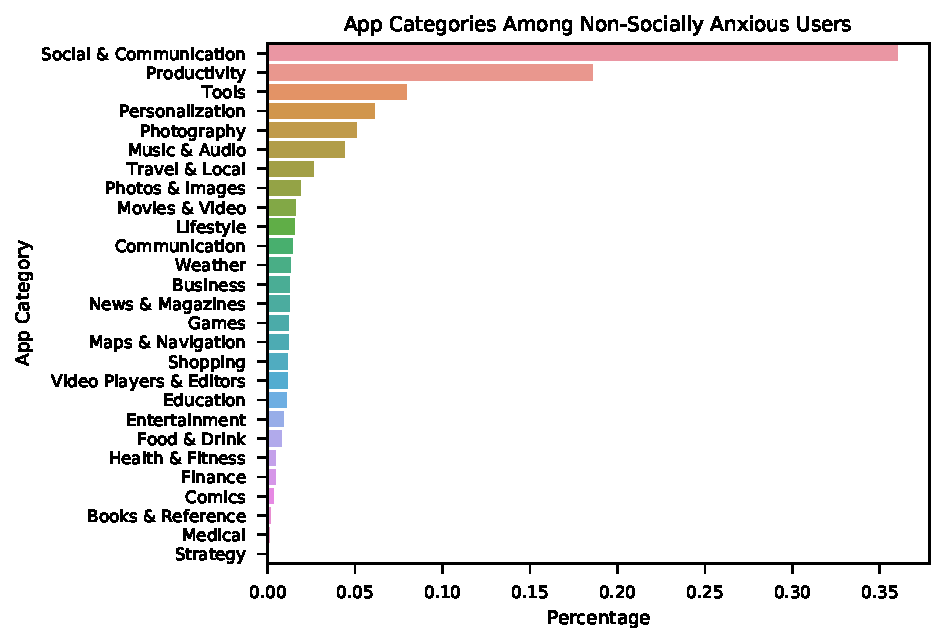
\includegraphics[width=\linewidth]{images/sessions/categories_among_non_anxious.pdf}
    \caption{This figure shows the distribution in application categories in non-anxious users. It is important to note that this distribution is very similar to the one in Figure  \ref{fig:session_app_categories}. }
    \label{fig:categories_among_non_anxious} 
\end{figure}

\begin{figure}[htb]
    \centering
    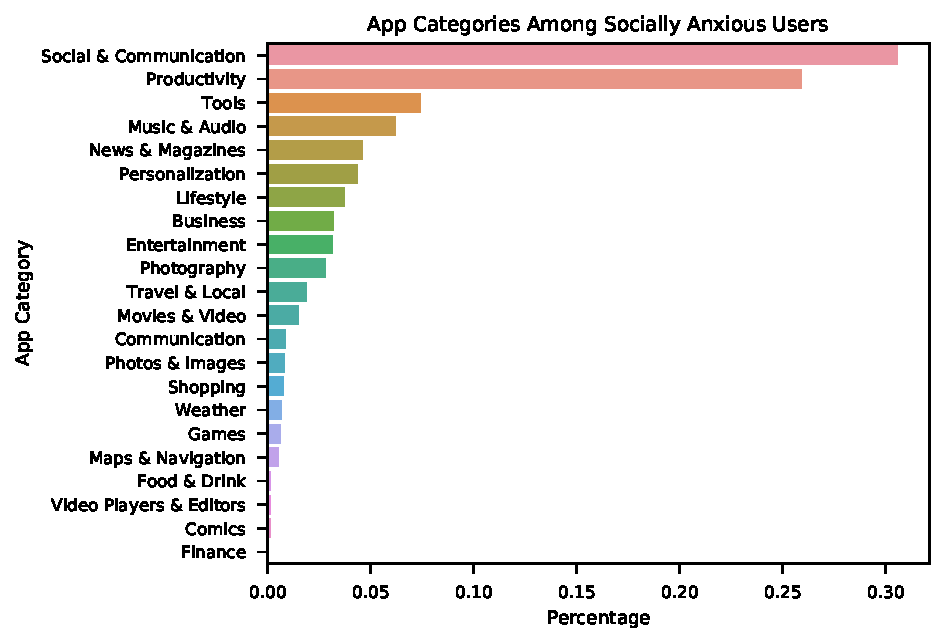
\includegraphics[width=\linewidth]{images/sessions/categories_among_anxious.pdf}
    \caption{This figure shows the distribution in application categories in socially anxious users. It is important to note that this distribution is slightly different than the one in Figure \ref{fig:session_app_categories}. The \textit{Productivity} category has a larger percentage overall, and the \textit{Social \& Communication} category is overall smaller.}
    \label{fig:categories_among_anxious} 
\end{figure}



\subsection{Classifier Performance}
A decision tree classifier was used to train a model on the features stated above. The tree used the Gini impurity measure and no maximum tree depth was set. A training and testing split of 80\%/20\% was used. Table \ref{table:session_metrics} shows the scores for the model. The overall accuracy of the model is \num{93}\%, which suggests that even though the features have a low correlation they may indicate if an individual has social anxiety or not. Since the class imbalance is low, up-sampling was not performed. Figure \ref{fig:session_matrix} shows the confusion matrix for the model. It indicates that the model was generally very accurate and predicted the wrong label only a small amount of times. The model was cross-validated with a stratified KFold strategy with 10 splits. Figure \ref{fig:session_learning_curve_dtree} show the classifier performance during the cross-validation. It can be seen that its performance increases logarithmically. Figure \ref{fig:session_roc_dtree} portrays the ROC score as 0.92, which indicates that the cross-validation testing was beneficial in checking the validity of the model. Figure \ref{fig:session_feature_importance_dtree} shows the importance of each feature in the model. Because there are only two features, it may be possible for the model to be overfitting around one of them, in this case \textit{totalTimeInForeground}.

\begin{table}[htb]
\centering
\begin{tabular}{@{}cccc@{}}
 & \textbf{Precision} & \textbf{Recall} & \textbf{F1} \\ \midrule
\textbf{0} & 0.94 & 0.95 & 0.94 \\
\textbf{1} & 0.92 & 0.91 & 0.91
\end{tabular}
\caption{This table shows the metrics for the decision tree classifier model for the application session usage data. The overall accuracy was 93\%.}
\label{table:session_metrics}
\end{table}

\begin{figure}[htb]
    \centering
    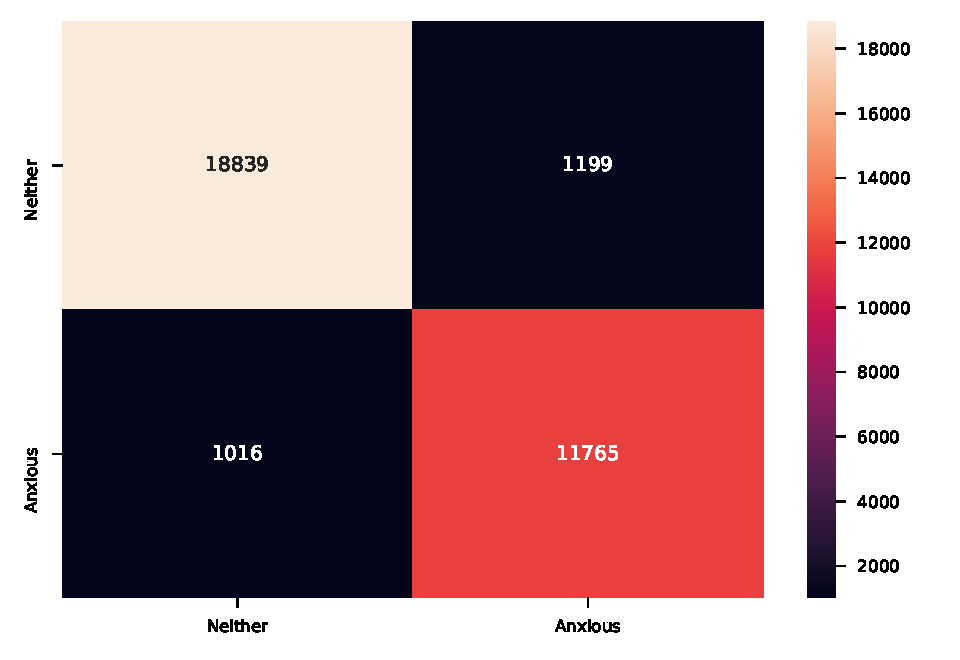
\includegraphics[width=0.75\linewidth]{images/sessions/heatmap_DecisionTreeSessions.pdf}
    \caption{This figure shows the confusion matrix for the decision tree classifier model for the application session usage data. The model had large accuracy in predicting the correct labels.}
    \label{fig:session_matrix} 
\end{figure}

\begin{figure}[htb]
    \centering
    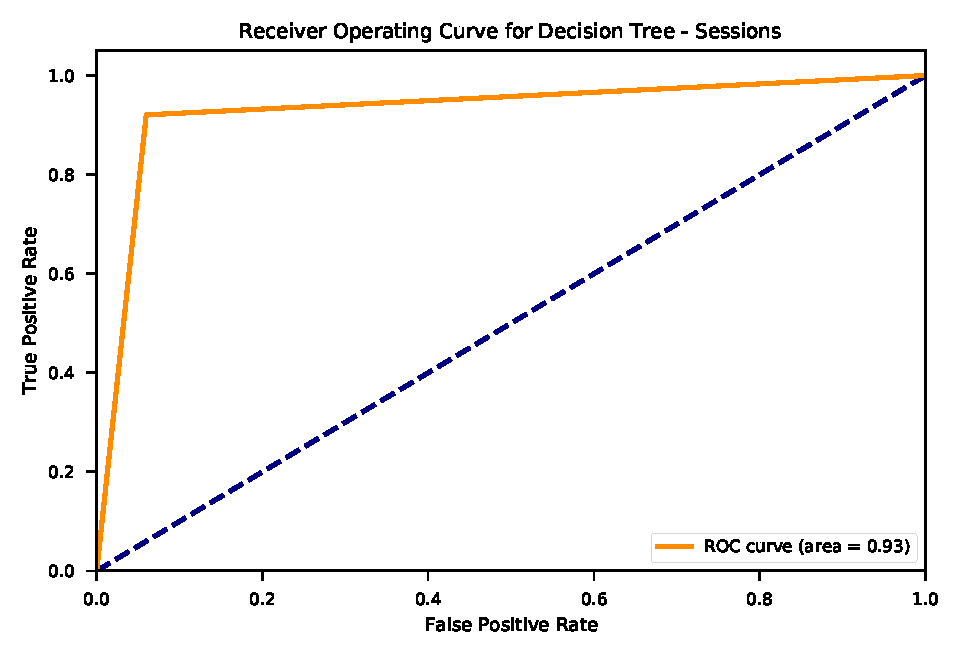
\includegraphics[width=0.75\linewidth]{images/sessions/roc_DecisionTreeSessions.pdf}
    \caption{This figure shows the receiver operating curve and its area underneath. A high area such as this indicates that the cross validation testing was very useful in checking the validity of the model.}
    \label{fig:session_roc_dtree} 
\end{figure}

\begin{figure}[htb]
    \centering
    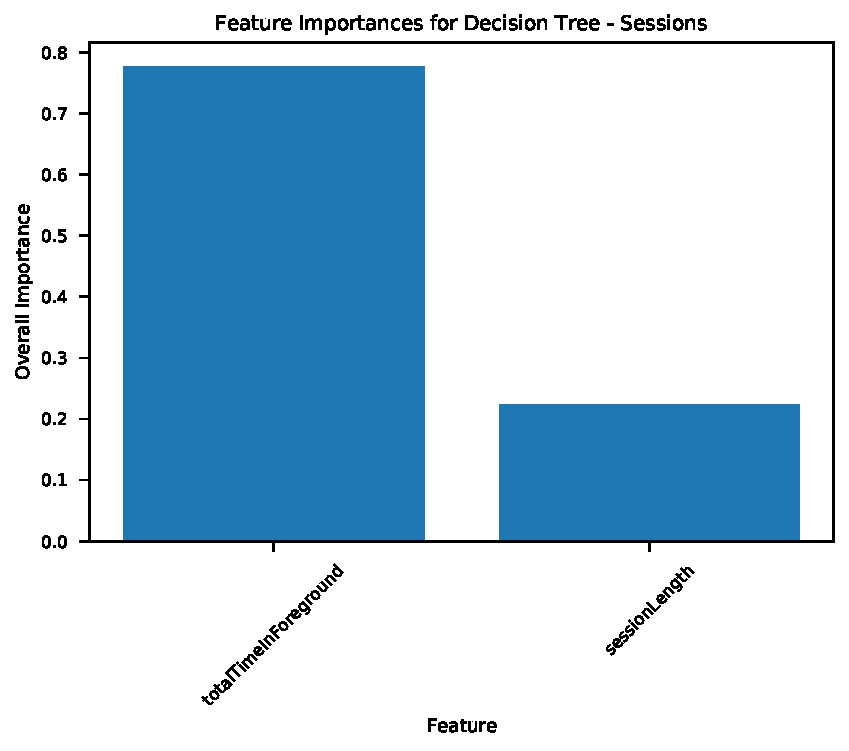
\includegraphics[width=0.70\linewidth]{images/sessions/feature_importance_DecisionTreeSessions.pdf}
    \caption{This figure shows the feature importance for the decision tree classifier. The feature totalTimeInForeground represents how long the application was visible to the individual.}
    \label{fig:session_feature_importance_dtree} 
\end{figure}

\begin{figure}[htbp]
    \centering
    \begin{subfigure}[b]{0.70\textwidth}
        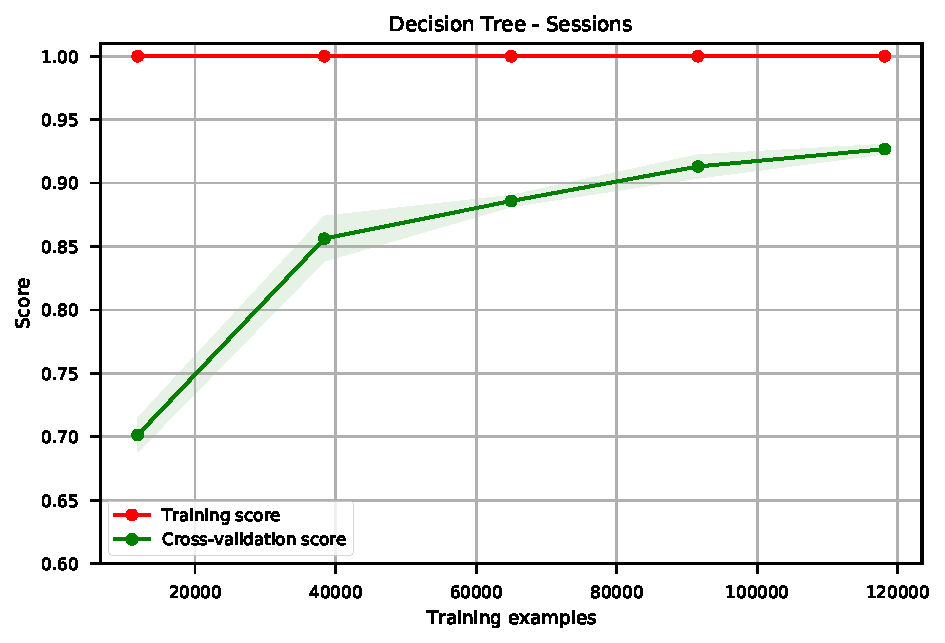
\includegraphics[width=\textwidth]{images/sessions/learning_curve_1_DecisionTreeSessions.pdf}
        \caption{}
        \label{fig:learning_curve_1_DecisionTreeSessions}
    \end{subfigure}
    \begin{subfigure}[b]{0.70\textwidth}
        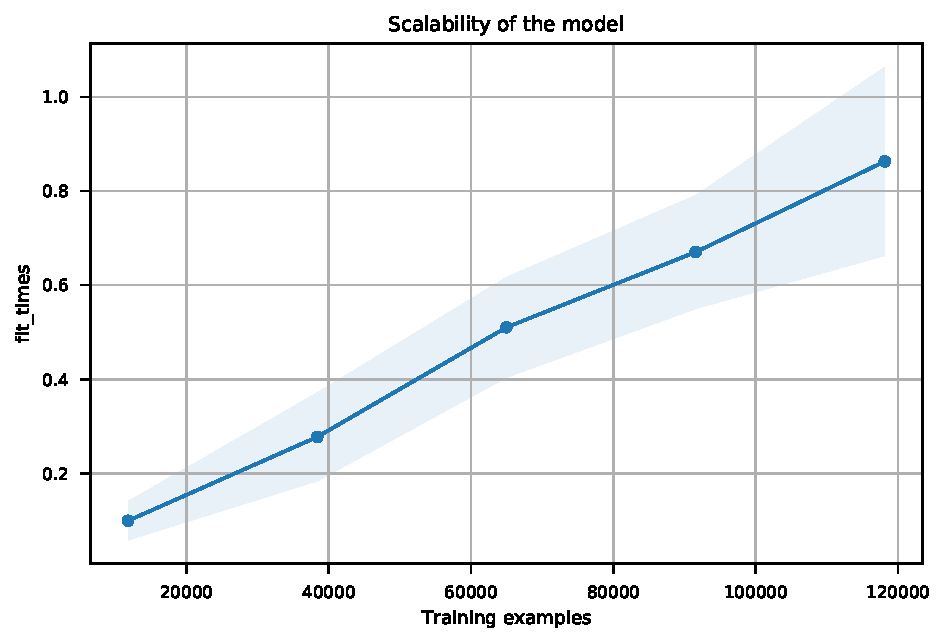
\includegraphics[width=\textwidth]{images/sessions/learning_curve_2_DecisionTreeSessions.pdf}
        \caption{}
        \label{fig:learning_curve_2_DecisionTreeSessions}
    \end{subfigure}
    \begin{subfigure}[b]{0.70\textwidth}
        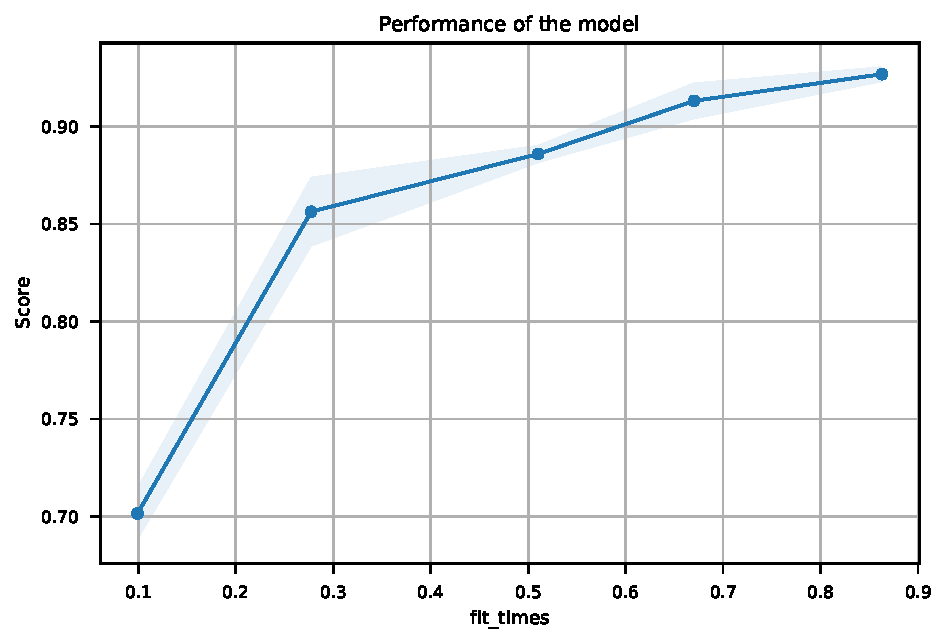
\includegraphics[width=\textwidth]{images/sessions/learning_curve_3_DecisionTreeSessions.pdf}
        \caption{}
        \label{fig:learning_curve_3_DecisionTreeSessions}
    \end{subfigure}
    \caption{This figure shows the performance of the decision tree classifier during cross-validation. The performance increases logarithmically as the training examples increase. There is a linear increase in the fit times as the training examples increase.}\label{fig:session_learning_curve_dtree}
\end{figure}


\subsection{Comparison With Other Classifiers}
The model above was compared to similar classifier models. The  Extra Trees Classifier\footnote{\url{https://scikit-learn.org/stable/modules/generated/sklearn.ensemble.ExtraTreesClassifier.html}} and Random Forest Classifier\footnote{\url{https://scikit-learn.org/stable/modules/generated/sklearn.ensemble.RandomForestClassifier.html}} were used. These alternative classifiers attempt to lower overfitting, improve accuracy, and scale better \citep{extra_trees_1, extra_trees_2, random_forests}. We wanted to see how the data would fare with these advanced classifiers. Table \ref{table:session_extra_classifier_metrics} shows the metrics of these three classifiers. Both of these ensemble classifiers perform slightly worse than the original decision tree model. This could be due to the ensemble methods trying to account for the inconsistencies in the features or data. Figures \ref{fig:session_extra_trees_matrix} and \ref{fig:session_random_forest_matrix} show the respective confusion matrix charts for the extra trees and random forest classifier models. The matrices show that there is a significantly higher amount of incorrect predictions. The extra trees classifier has an accuracy of \num{86}\% and the random forest classifier has an accuracy of \num{87}\%. Both classifiers have \textit{totalTimeInForeground} as the most important feature, as seen in Appendix figures \ref{fig:session_extra_trees_feature} and \ref{fig:session_random_forest_feature} show that the respective importance values for the extra trees and random forest model features are closer to being even. Additionally, Appendix figures \ref{fig:session_extra_trees_learning_curve} and \ref{fig:session_random_forest_learning_curve} respectively show the classifiers' performance during cross-validation. Both classifiers produce lower accuracy scores compared to the original decision trees. Likewise, both classifiers have a logarithmic performance when it comes to fit times and the score produced as the fit time increases. Appendix figures \ref{fig:session_extra_trees_roc} and \ref{fig:session_random_forest_roc} show the respective ROC curves of the extra tree and random forest classifier.

\begin{table}[htb]
\centering
\begin{tabular}{@{}lccc|ccc@{}}
\toprule
 & \multicolumn{3}{c|}{\textbf{Extra Trees Classifier}} & \multicolumn{3}{c|}{\textbf{Random Forest Classifier}} \\ \midrule
 & \textbf{Precision} & \textbf{Recall} & \textbf{F1} & \textbf{Precision} & \textbf{Recall} & \textbf{F1} \\
\multicolumn{1}{c}{\textbf{0}} & 0.92 & 0.86 & 0.89 & 0.92 & 0.87 & 0.90 \\
\multicolumn{1}{c}{\textbf{1}} & 0.77 & 0.87 & 0.82 & 0.80 & 0.88 & 0.83 \\ \bottomrule
\end{tabular}
\caption{This table shows the metrics the two other classifiers that were trained with the application session usage data. The random forest has slightly better scores overall. Its performance is worse than the original decision tree classifier, whose metrics can be seen in table \ref{table:session_metrics}.}
\label{table:session_extra_classifier_metrics}
\end{table}

% MOVED TO APPENDIX
\begin{figure}[htb]
    \centering
    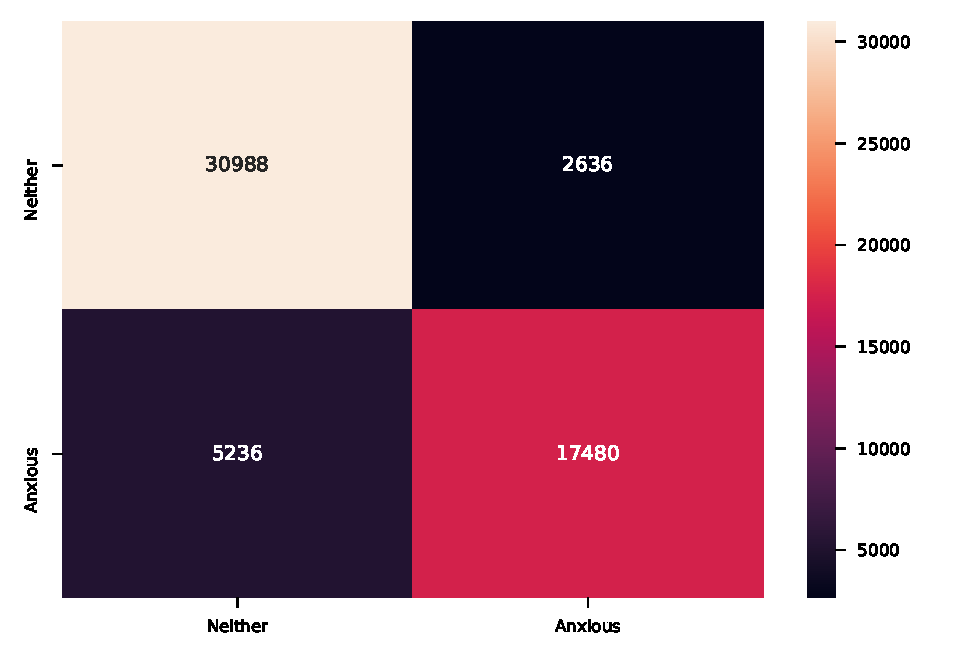
\includegraphics[width=0.80\linewidth]{images/sessions/heatmap_EnsembleExtraTreesSessions.pdf}
    \caption{This figure shows the confusion matrix for the extra trees classifier. It can be seen that there is a significantly higher amount of incorrect predictions.}
    \label{fig:session_extra_trees_matrix} 
\end{figure}

\begin{figure}[htb]
    \centering
    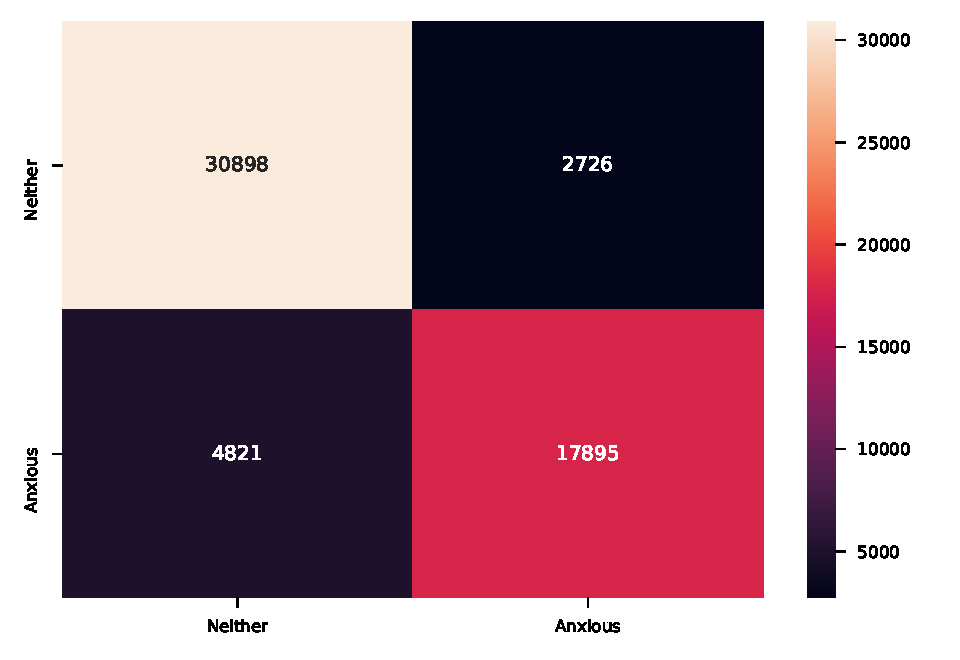
\includegraphics[width=0.80\linewidth]{images/sessions/heatmap_EnsembleRandomForestSessions.pdf}
    \caption{This figure shows the confusion matrix for the random forest classifier. It can be seen that there is a significantly higher amount of incorrect predictions.}
    \label{fig:session_random_forest_matrix} 
\end{figure}

\subsection{Issues and Discussion}
We expected for the application usage session data to have a class imbalance for the SIAS scores. The 2:3 ratio of non-socially anxious individuals to socially anxious individuals is better than expected. Because of this, up-sampling was not considered. Additionally, we expected the decision tree to perform adequately due to research by \citet{apple_patterns}. While \citet{apple_patterns} did not look at social anxiety, they did look at the relationship between cognitive health and smartphone usage by examining each individual's application session data.

The application category was a respectable spread. It was to be expected that the most used type would be \textit{Social \& Communication}, as shown by previous research \citet{different_users_thru_app_usage, angry_birds_study}. Some applications had categories that did not seem to be in line with what the application offered. For example, both Chrome and Brave Browser were labelled as \textit{Social \& Communication} which arguably is not the main purpose of these applications. Additionally, the \textit{Productivity} category among socially anxious users had a larger presence compared to non-socially anxious users. This suggests that socially anxious users may be more inclined to engage in activities that keep them busy and do not require interaction with other individuals.

Table \ref{table:session_times_dtree} shows the average time for the top two application categories in individuals. The table suggests that socially anxious people may spend less time overall with applications that are social in nature, such as those in the \textit{Social \& Communication} category.

\begin{table}[htbp]
\centering
\begin{tabular}{@{}cccc@{}}
\toprule
\multicolumn{4}{c}{\textbf{Average Time in Foreground (minutes) in Individuals for the Top Two Categories}} \\ \midrule
\multicolumn{2}{c|}{\textbf{Non-Socially Anxious}} & \multicolumn{2}{c|}{\textbf{Socially Anxious}} \\ \midrule
\textbf{Social \& Communication} & \multicolumn{1}{c|}{\textbf{Productivity}} & \textbf{Social \& Communication} & \textbf{Productivity} \\
13 & \multicolumn{1}{c|}{3} & 11 & 2 \\ \bottomrule
\end{tabular}
\caption{This table shows the average time for the top two categories in both non-socially anxious and socially anxious individuals. It can be seen that in socially anxious people the overall times are lower, but as seen in Figure \ref{fig:categories_among_anxious} the percentage for these two categories is lower overall.}
\label{table:session_times_dtree}
\end{table}

We wanted to explore the usage of other classifiers, to see how the original decision tree model would compare. We suspected that the decision tree may over-fit, and so it made sense to use classifiers that use similar techniques but are much more thorough and advanced. With the decision tree only using two features that have a low correlation to the SIAS score, it gives rise to the thought that the original model is not entirely valid and may be incorrectly fitting the data. The usage of the Extra Trees and Random Forest classifier helped to show that there is some validity to the decision tree but that it should not be relied on entirely. Additionally, extra trees and random forest allow for more in-depth parameter tuning, which was not done in this study due to time constraint.

Overall, it can be said that application session usage data could be used to predict social anxiety. To that end, we would suggest exploring additional non-tree based classifiers that can deal with class imbalance and data impurities better. While this would increase complexity and require hyper-parameter tuning, we argue that it could be much more useful than the standard decision tree. We did achieve a high score with the decision tree model but suspect that it is not entirely valid. The lower performance with the Extra Trees and Random Forest show that there should be additional features as well as model tuning. Additionally, implementing a text embedding method like \cite{apple_patterns} could result in further accuracy and validity.


\section{Requirements Validation}
The final stage of the evaluation process was to see if the functional and non-functional requirements in chapter \ref{requirements} were met. Requirements that fall under the \textit{Won't Have This Time} will not be included in the evaluation because they were not part of the scope of the project.

Overall, 23 out of 28 \textit{Must Have}, \textit{Should Have}, and \textit{Could Have} requirements were met at the end of the project. This is approximately 82\%. All of the 13 \textit{Must Have} requirements were met; 7 of the 10 \textit{Should Have} requirements were met; only 3 of the 5 \textit{Could Have} requirements were met. The \textit{Should Have} requirements that were not met were \textbf{8}, restart the application if it crashes unexpectedly, \textbf{9}, collect text message data, and \textbf{25}, encrypt the data on the device. The \textit{Could Have} requirements that were not met were \textbf{11}, integrate individual activity recognition, and \textbf{17}, find the best classifier with the best parameters and features. These requirements were not met due to time constraints. At the same time they could be beneficial and should be considered for future work.


\section{Summary}
This chapter looked at how the evaluation was conducted for this project. First, a short description of the user trials was given. A decision tree model was created for location data and compared to previous research. The results were similar to what \cite{wood, boukhechba} achieved, but our data suffered from a large class imbalance and was inconsistent in the gathering rate. Afterwards, session usage data was looked at and a decision tree model was created. The data did not suffer from a large class imbalance. Initially, the model performed very well but we suspect that it may be overfitting on some features, even with cross-validation performed. We further trained an Extra Trees and Random Forest classifier to compare with, and saw that the score was lower with those. This leads us to believe that the decision tree model needs more features than what it currently has and that future research should use more advanced and flexible classifiers. Finally, we looked at the requirements that were met and that were not met.


%==================================================================================================================================
\chapter{Conclusion} \label{conclusion}
This paper discussed the motivation and aim of the study. We wanted to see if application session usage can be used to accurately predict whether an individual has social anxiety. We listed the requirements that were gathered for all parts of the project and then revealed how we designed and further implemented them. Then we provided an extensive evaluation where we compared location data with past research and later showed how our model performed with the application usage data. The final chapter in this paper will provide a summary of the entire project and look at what future work could be carried out. Finally, it will conclude with a personal reflection.

\section{Summary}
We wanted to find out if application session usage can be used to accurately predict whether an individual has social anxiety. To accomplish this, we studied past research to identify what has already been done. We saw that various mobile-based sensors can be a useful indicator in identifying issues such as stress and social anxiety. Additionally, we saw that less intrusive data collection produces more positive results as the individuals do not alter their behaviour unconsciously. Other research indicated that analysing application usage chains in sessions provides high accuracy in predicting individuals with cognitive impairments. This led us look at how application usage sessions can be used to predict social anxiety.

We built an Android application that collected location and application session usage data. The location data was comprised of latitude, longitude, and timestamp data points. The application session usage data was comprised of application names, categories, and usage duration data points. The application collected this data continuously in the background. The individual was asked to do a SIAS test as well. This allowed us to link their social anxiety level with collected data.

We had a remote server and database to process the collected data. We followed GDPR guidelines and enabled encryption for the data at rest and during transit. We also enabled TLS with a Let's Encrypt certificate. All these precautions were done to ensure that data was not lost or at risk.

Each location was converted into a category based on the address that was returned by reverse geocoding the latitude and longitude pairs. A classifier was trained on the location categories and compared it with previous research. The results that we achieved were similar to past research and so we concluded that location data can be a viable indicator of social anxiety.

We created a separate Decision Tree, Extra Trees, and Random Forest classifier models from the application usage session data. We achieved the highest accuracy, 93\%, with the decision tree model. The model was cross-validated and the results were positive. Nevertheless we were still wary that the tree may be overfitting or may not have enough features, and hence used the Extra Trees and Random Forest classifiers. These two are more advanced and try to account for the issues that a regular Decision Tree suffers from. Extra Trees and Random Forest achieved 86\% and 87\% accuracy respectively.

We concluded that application usage session data could be used to predict social anxiety in an individual. Based on this, we hypothesise that application usage data could be further used as an indicator of other serious health conditions but did not explore this due to the ethical challenges involved. Additionally, we concluded that it may be beneficial to use a more advanced classifier that can account for overfitting and other issues that may stem from the data.

\section{Future work}
There is potential in implementing a text embedding method, such as the one from \citet{apple_patterns}, when exploring application usage session data. This could allow for more actionable conclusions and better accuracy. Future work could include a mix of text embedding for application names and categories as well as various usage times.

Future research could also look at using call and text data coupled with location and application usage statistics. We believe that knowing the location during each session could be highly beneficial, as it could potentially reveal links between applications and the current location that they are used in. For example, we hypothesise that socially anxious individuals may use \textit{Social \& Communication} related applications when in a social setting to avoid speaking to other physical individuals near them.

Participant data could also be gathered from Apple devices alongside Android. This would provide a much larger insight into the broader general population. Additionally, gathering data from a wider age group could provide insight into how application usage session data changes over time. Past research has shown that usage data changes with adults over time, and it could be worthy to explore how socially anxious age groups change over time. The current study surveyed only university students with Android devices. Implementing federated machine learning could allow data processing model training to occur on participant devices. This would be ideal for preserving personal data and privacy.

Further future work could attempt to link application session usage data to other serious health conditions.

\section{Reflection}
This project taught me considerably about how to organise and manage my time. This was my first time working on a year-long project and I was unsure about a lot of aspects. I would like to express my sincere appreciation to my supervisor who provided a lot of guidance and support during the project. I was able to identify techniques that worked for me along the way. For example, using the GitHub wiki page was immensely beneficial. I used it to track my time as well as write notes. 

A key takeaway was that I need to be more careful when running user trials. I confused two Android methods for the location data collection and ended up taking the wrong timestamp. This resulted in the first trial being completely invalidated. Additionally, writing this paper gave me valuable insight into how to structure my thoughts and present my results.

I gained extensive experience in writing Android applications as well as using data science libraries. Both Android and Scikit-learn are complex but I learned that they can be used with great success.

%==================================================================================================================================
%  APPENDICES  

\begin{appendices}
\chapter{Social Interaction Anxiety Scale Questions}

\begin{figure}[htb]
    \centering
    \begin{enumerate}
        \item I get nervous if I have to speak with someone in authority.
        \item I have difficulty making eye contact with others.
        \item I become tense if I have to talk about myself or my feelings.
        \item I find it difficult to mix comfortably with the people I work with.
        \item I find it easy to make friends my own age.
        \item I tense up if I meet an acquaintance in the street.
        \item When mixing socially, I am uncomfortable.
        \item I feel tense if I am alone with just one other person.
        \item I am at ease meeting people at parties.
        \item I have difficulty talking with other people.
        \item I find it easy to think of things to talk about.
        \item I worry about expressing myself in case I appear awkward.
        \item I find it difficult to disagree with another’s point of view.
        \item I have difficulty talking to attractive persons of the opposite sex.
        \item I find myself worrying that I won’t know what to say in social situations.
        \item I am nervous mixing with people I don’t know well.
        \item I feel I’ll say something embarrassing when talking.
        \item When mixing in a group, I find myself worrying I will be ignored.
        \item I am tense mixing in a group.
        \item I am unsure whether to greet someone I know only slightly.
    \end{enumerate}
    \caption{This figure shows the SIAS self-report questions that were presented to the participants. In some cases, the wording may be outdated. Question 14 is an example.}
    \label{fig:sias_questions} 
\end{figure}

\chapter{Location Categories and SIAS Score Correlation}
\begin{figure}[htb]
    \centering
    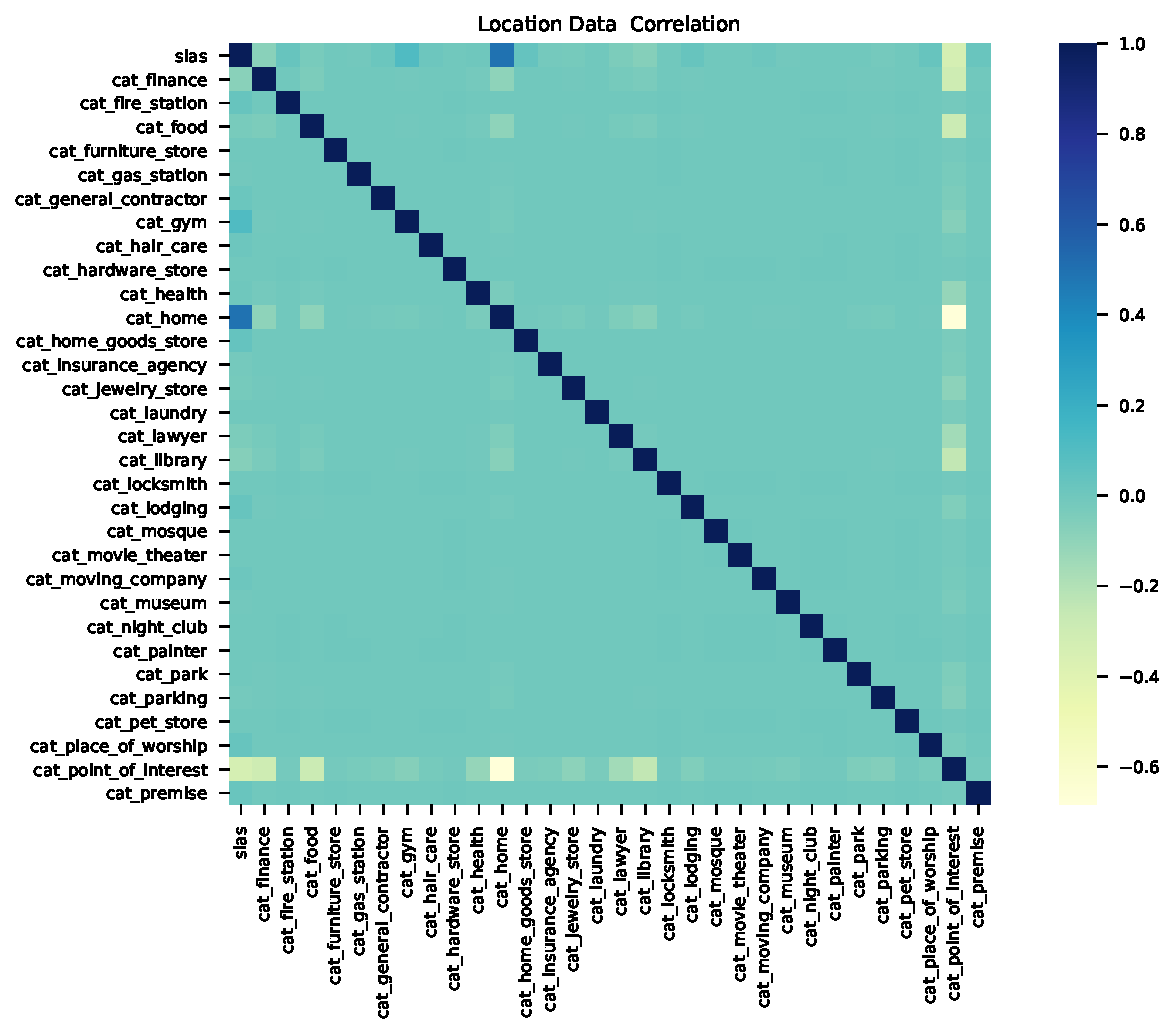
\includegraphics[width=1.1\linewidth]{images/location/correlation_LocationData.pdf}
    \caption{This figure shows the correlations between the categories and the SIAS score. A majority of categories have little to no correlation, and some have negative. Category \textit{home} has the most significant positive correlation with the SIAS score.}
    \label{fig:location_category_correlations} 
\end{figure}

\chapter{Location Classifier Statistics with SMOTE Up-sampling}
\begin{figure}[htb]
    \centering
    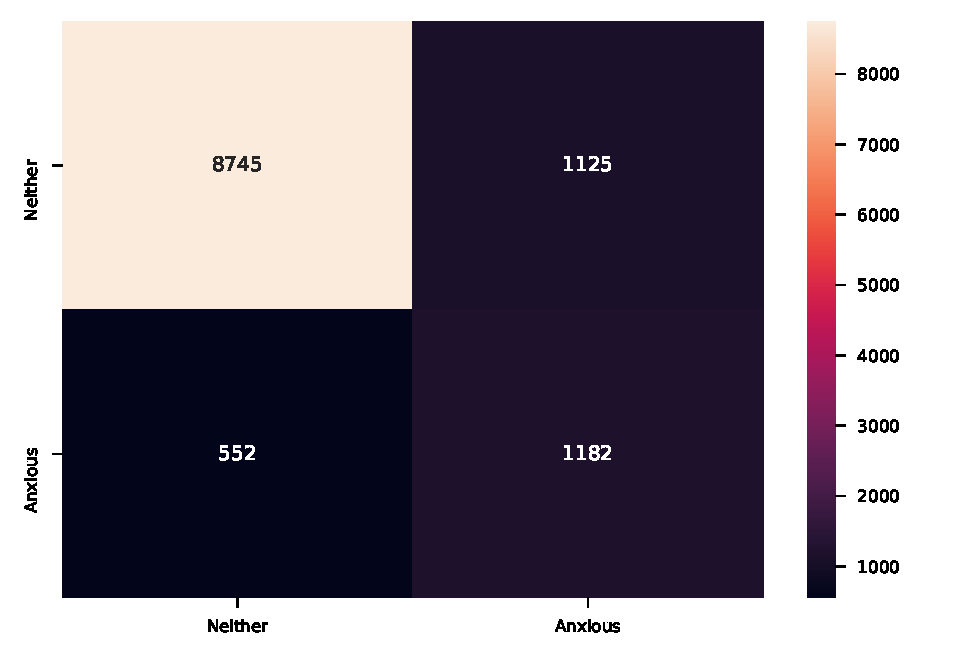
\includegraphics[width=\linewidth]{images/location/heatmap_Decision_Tree_Locations_sm.pdf}
    \caption{This figure shows the confusion matrix for the decision tree classifier model with SMOTE up-sampling. The prediction accuracy for socially anxious individuals is still significantly low and suggests that up-sampling was not entirely effective.}
    \label{fig:location_sm_matrix} 
\end{figure}

\begin{figure}[htb]
    \centering
    \noindent\makebox[\textwidth]{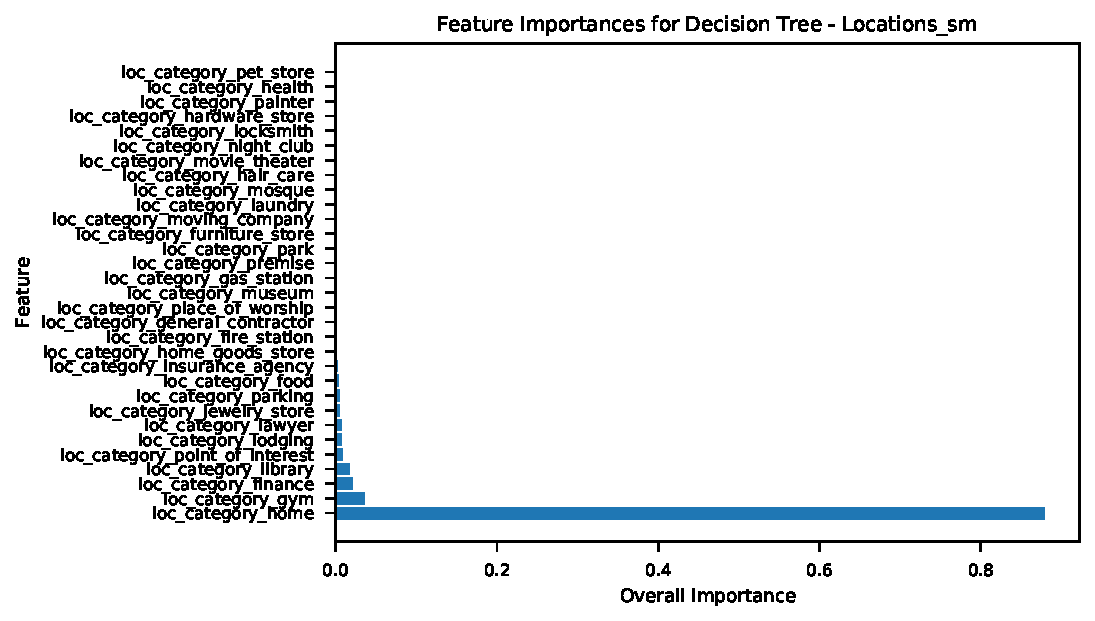
\includegraphics[width=1.08\linewidth]{images/location/feature_importance_Decision_Tree_Locations_sm.pdf}}
    \caption{This figure shows the feature importance for the decision tree classifier model with SMOTE up-sampling. It is almost identical to the feature importance graph for the model without up-sampling.}
    \label{fig:location_sm_feature_importance} 
\end{figure}

\begin{figure}[htbp]
    \centering
    \begin{subfigure}[b]{0.70\textwidth}
        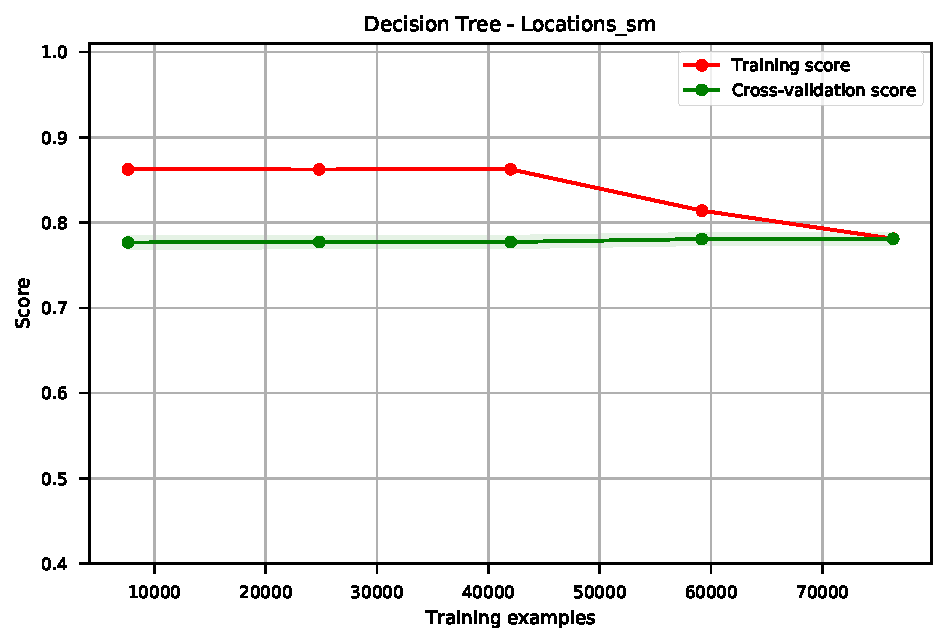
\includegraphics[width=\textwidth]{images/location/learning_curve_1_DecisionTreeLocations_sm.pdf}
        \caption{It seems that increasing the training examples leads to a convergence of the cross-validation and training scores.}
        \label{fig:learning_curve_1_DecisionTreeLocations_sm}
    \end{subfigure}
    \begin{subfigure}[b]{0.70\textwidth}
        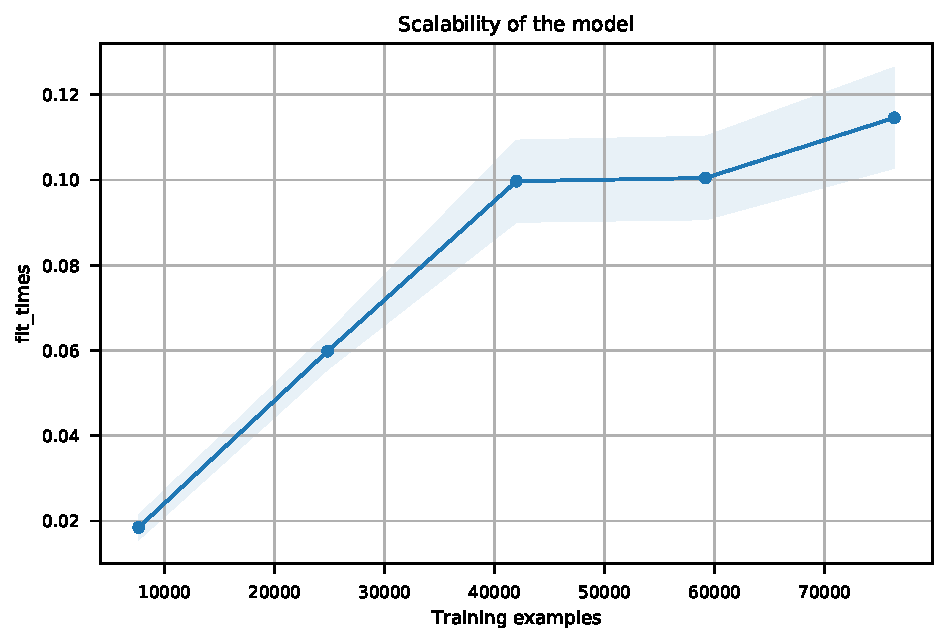
\includegraphics[width=\textwidth]{images/location/learning_curve_2_DecisionTreeLocations_sm.pdf}
        \caption{Scalability increases linearly for the most part.}
        \label{fig:learning_curve_2_DecisionTreeLocations_sm}
    \end{subfigure}
    \begin{subfigure}[b]{0.70\textwidth}
        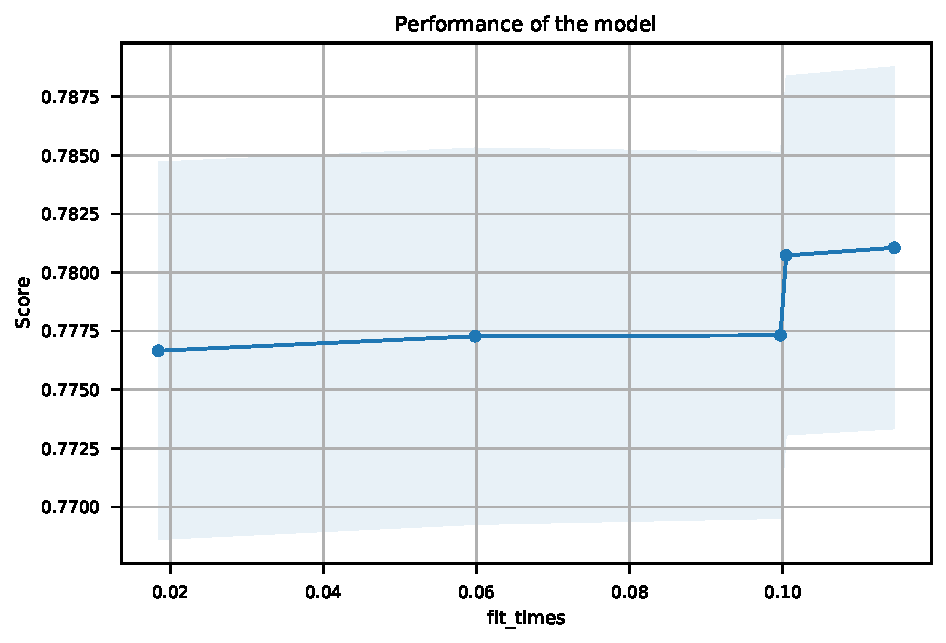
\includegraphics[width=\textwidth]{images/location/learning_curve_3_DecisionTreeLocations_sm.pdf}
        \caption{The performance does not seem to increase and may in fact be unstable.}
        \label{fig:learning_curve_3_DecisionTreeLocations_sm}
    \end{subfigure}
    \caption{This figure shows the cross-validation results of the decision tree classifier model with SMOTE up-sampling. It can be seen that there is a reduction in performance as the training sizes increase. Up-sampling may confuse the classifier if the original data suffered from other issues besides class imbalance.}\label{fig:location_sm_kfold}
\end{figure}

\begin{figure}[htbp]
    \centering
    \begin{subfigure}[b]{0.70\textwidth}
        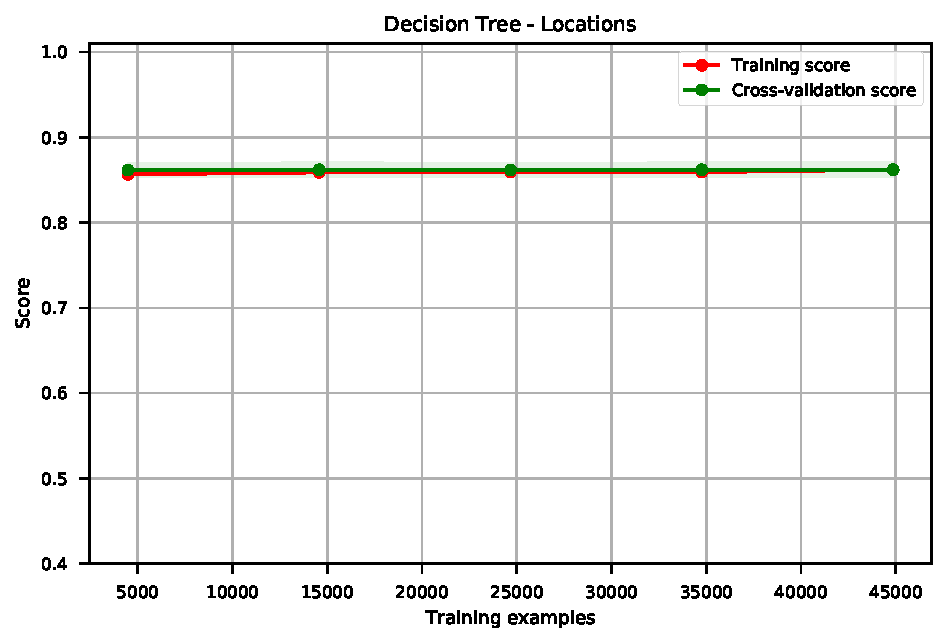
\includegraphics[width=\textwidth]{images/location/learning_curve_1_DecisionTreeLocations.pdf}
        \caption{The performance of the validation and testing are very similar.}
        \label{fig:learning_curve_1_DecisionTreeLocations}
    \end{subfigure}
    \begin{subfigure}[b]{0.70\textwidth}
        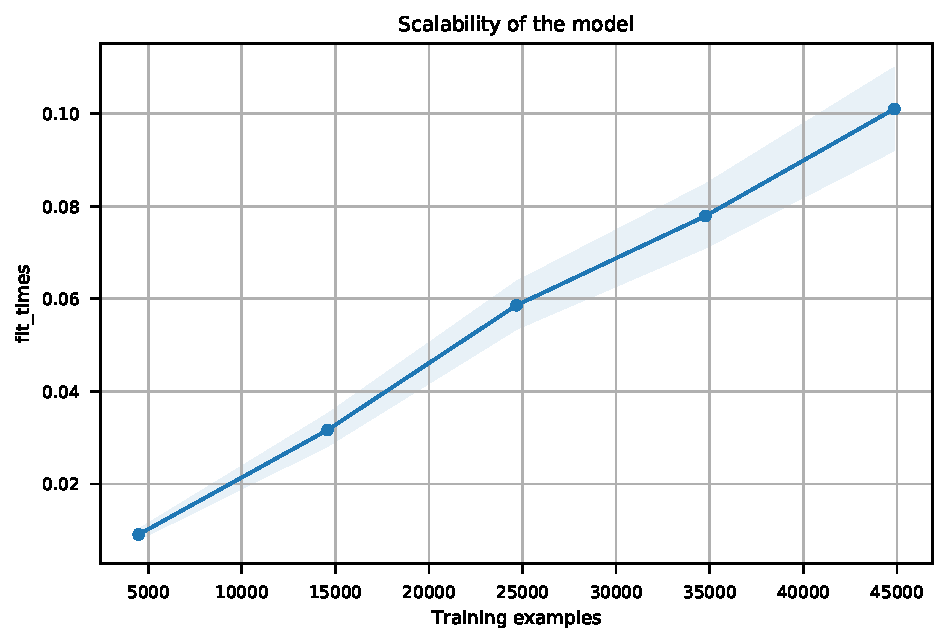
\includegraphics[width=\textwidth]{images/location/learning_curve_2_DecisionTreeLocations.pdf}
        \caption{The fit times increase as the training examples increase.}
        \label{fig:learning_curve_2_DecisionTreeLocations}
    \end{subfigure}
    \begin{subfigure}[b]{0.70\textwidth}
        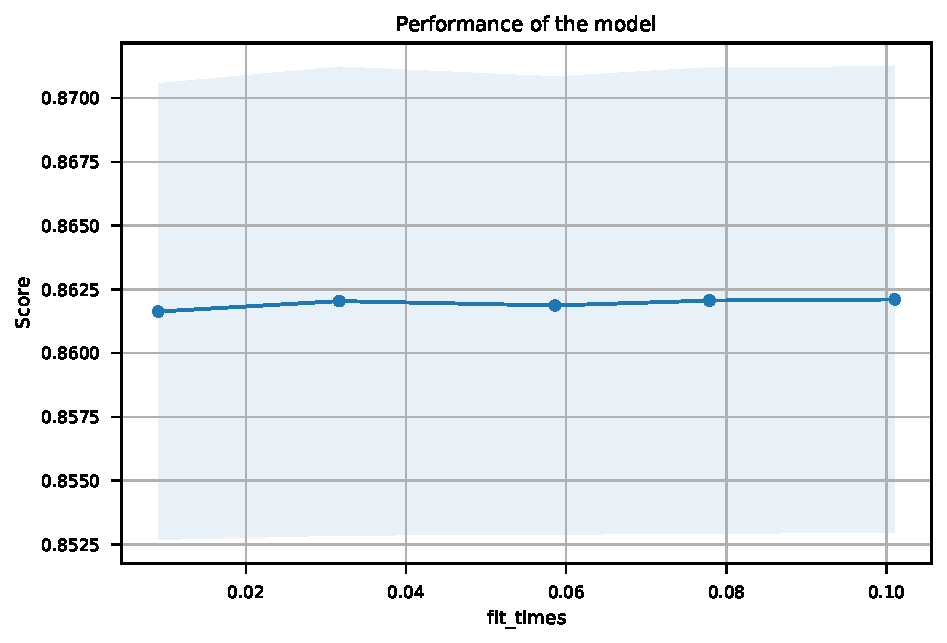
\includegraphics[width=\textwidth]{images/location/learning_curve_3_DecisionTreeLocations.pdf}
        \caption{The performance does not change much with fit times.}
        \label{fig:learning_curve_3_DecisionTreeLocations}
    \end{subfigure}
    \caption{This figure shows the performance of the classifier during the cross-validation. The scalability is linear with the size of the training examples but the score does not seem to vary much as the size and training times increase.}\label{fig:location_no_upsampling_kfold}
\end{figure}

\chapter{Extra Trees Classifier Graphs}

\begin{figure}[htb]
    \centering
    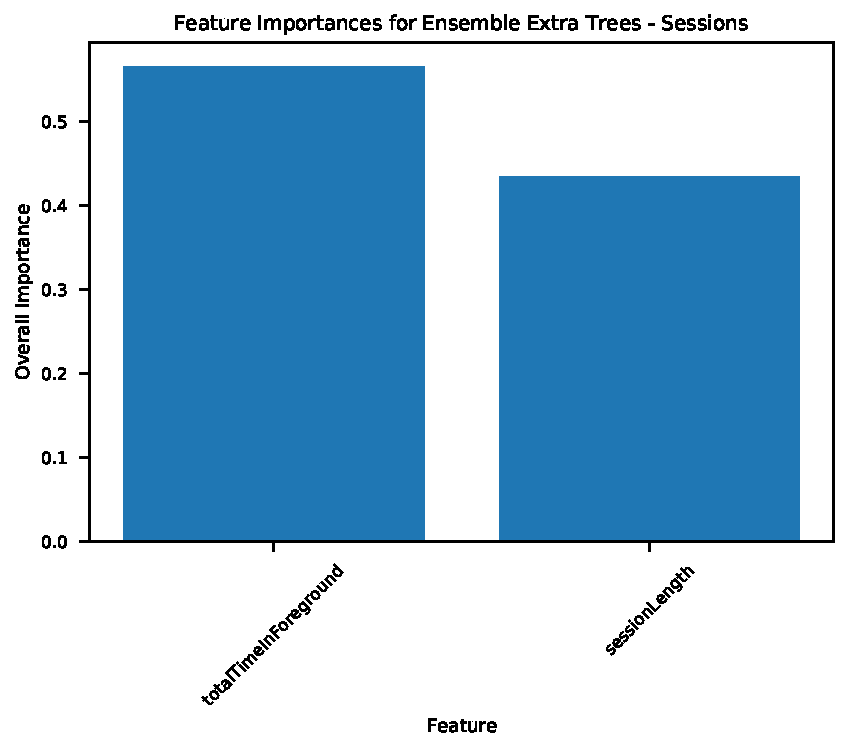
\includegraphics[width=\linewidth]{images/sessions/feature_importance_EnsembleExtraTreesSessions.pdf}
    \caption{This figure shows the feature importance data for the extra trees classifier. It is important to see that the feature importances are close to being identically important, unlike the original decision tree model.}
    \label{fig:session_extra_trees_feature} 
\end{figure}

\begin{figure}[htb]
    \centering
    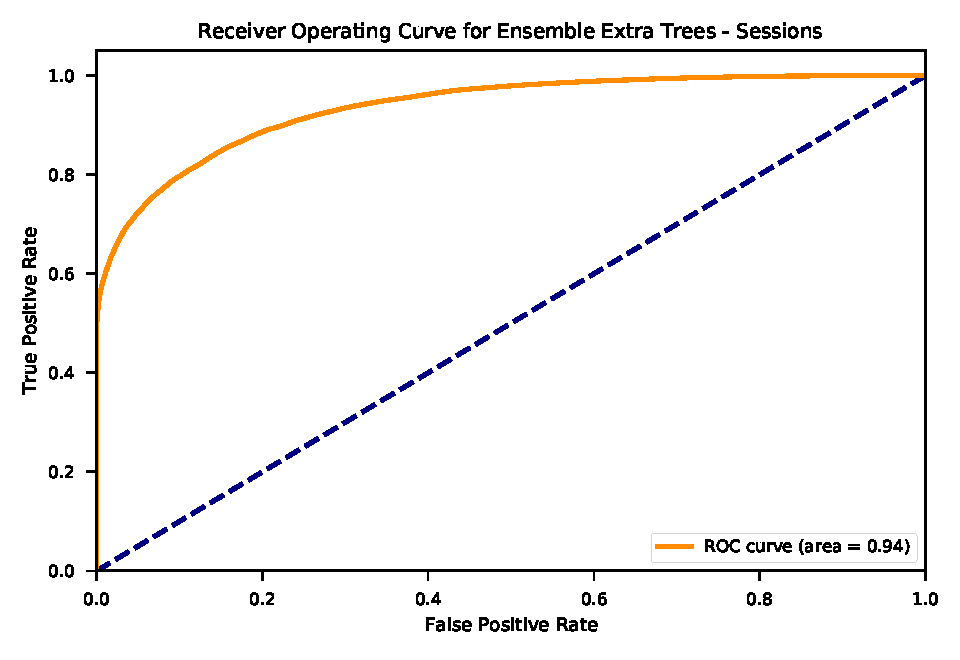
\includegraphics[width=\linewidth]{images/sessions/roc_EnsembleExtraTreesSessions.pdf}
    \caption{This figure shows the receiver operating curve and the respective area for the extra trees classifier. The curve area is almost 1, showing that the cross-validation was a useful test.}
    \label{fig:session_extra_trees_roc} 
\end{figure}

\begin{figure}[htbp]
    \centering
    \begin{subfigure}[b]{0.70\textwidth}
        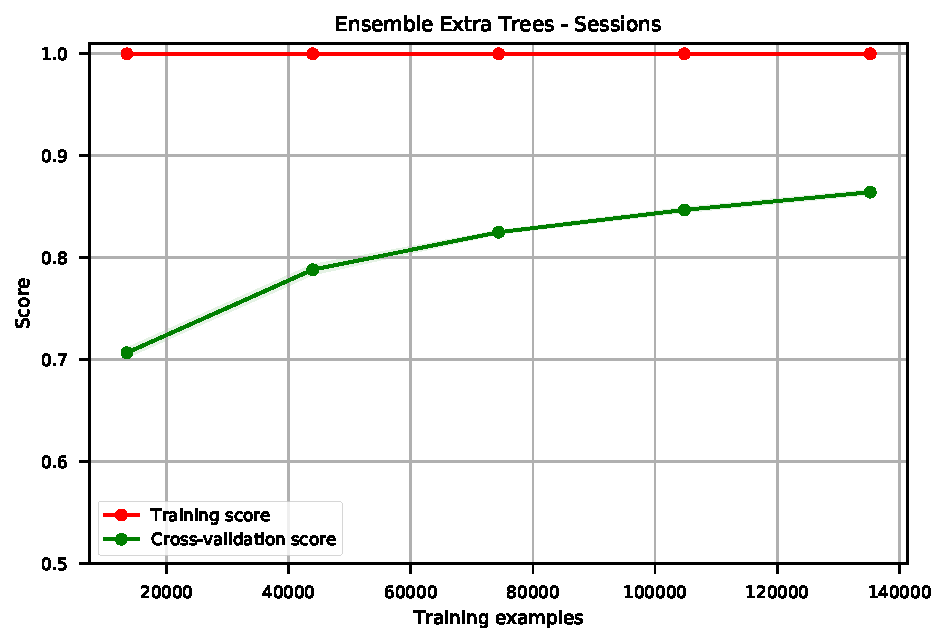
\includegraphics[width=\textwidth]{images/sessions/learning_curve_1_EnsembleExtraTreesSessions.pdf}
        \caption{The validation score increases logarithmically.}
        \label{fig:learning_curve_1_EnsembleExtraTreesSessions}
    \end{subfigure}
    \begin{subfigure}[b]{0.70\textwidth}
        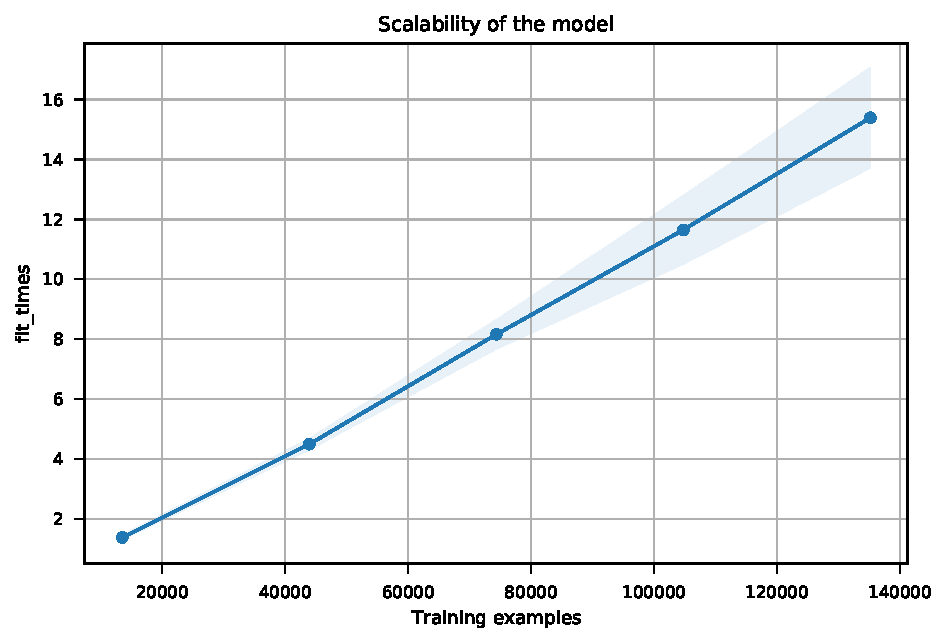
\includegraphics[width=\textwidth]{images/sessions/learning_curve_2_EnsembleExtraTreesSessions.pdf}
        \caption{The scalability of the model increases linearly.}
        \label{fig:learning_curve_2_EnsembleExtraTreesSessions}
    \end{subfigure}
    \begin{subfigure}[b]{0.70\textwidth}
        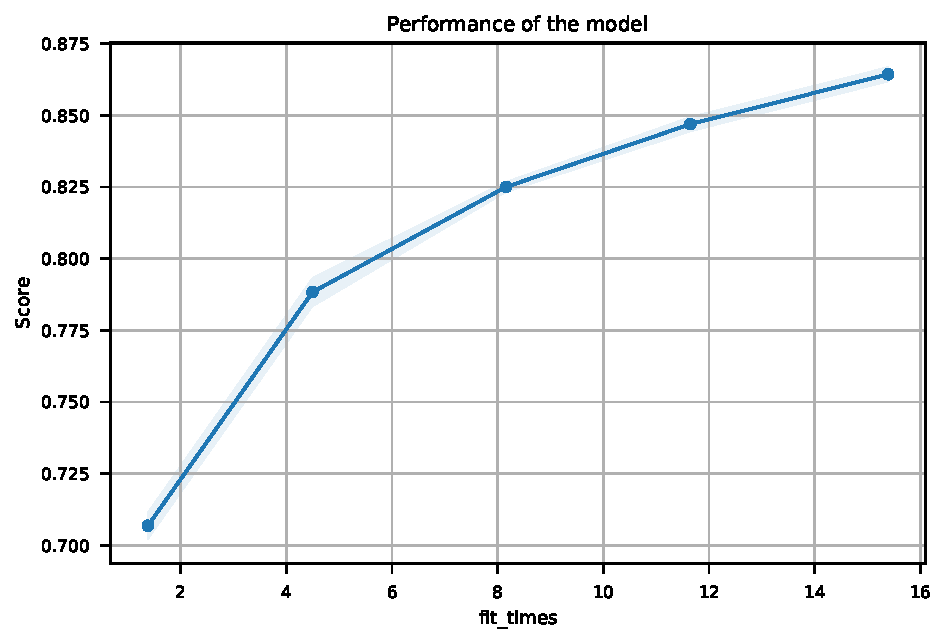
\includegraphics[width=\textwidth]{images/sessions/learning_curve_3_EnsembleExtraTreesSessions.pdf}
        \caption{The performance of the model increases logarithmically.}
        \label{fig:learning_curve_3_EnsembleExtraTreesSessions}
    \end{subfigure}
    \caption{This figure shows the performance of the extra trees classifier during cross-validation. The score increases by a small factor as the training examples increase. It is not logarithmic as the original decision tree model. The fit time increases linearly with the training examples. The fit times increase logarithmically with the score.}
    \label{fig:session_extra_trees_learning_curve}
\end{figure}

\chapter{Random Forest Classifier Graphs}

\begin{figure}[htb]
    \centering
    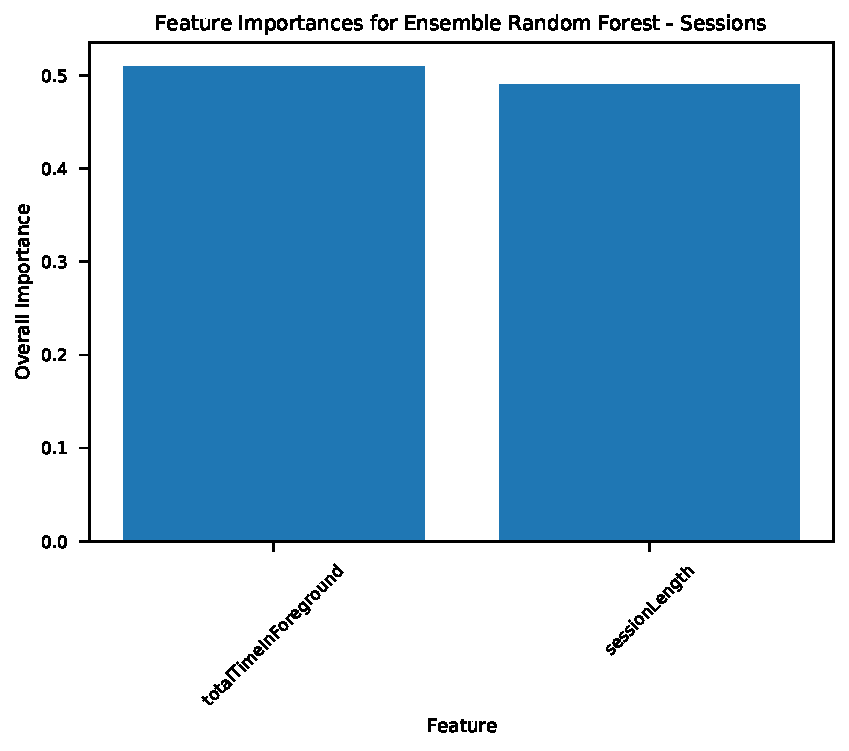
\includegraphics[width=0.75\linewidth]{images/sessions/feature_importance_EnsembleRandomForestSessions.pdf}
    \caption{This figure shows the feature importance data for the random forest classifier. It is important to see that the features are almost equally important, unlike the original decision tree model.}
    \label{fig:session_random_forest_feature} 
\end{figure}

\begin{figure}[htb]
    \centering
    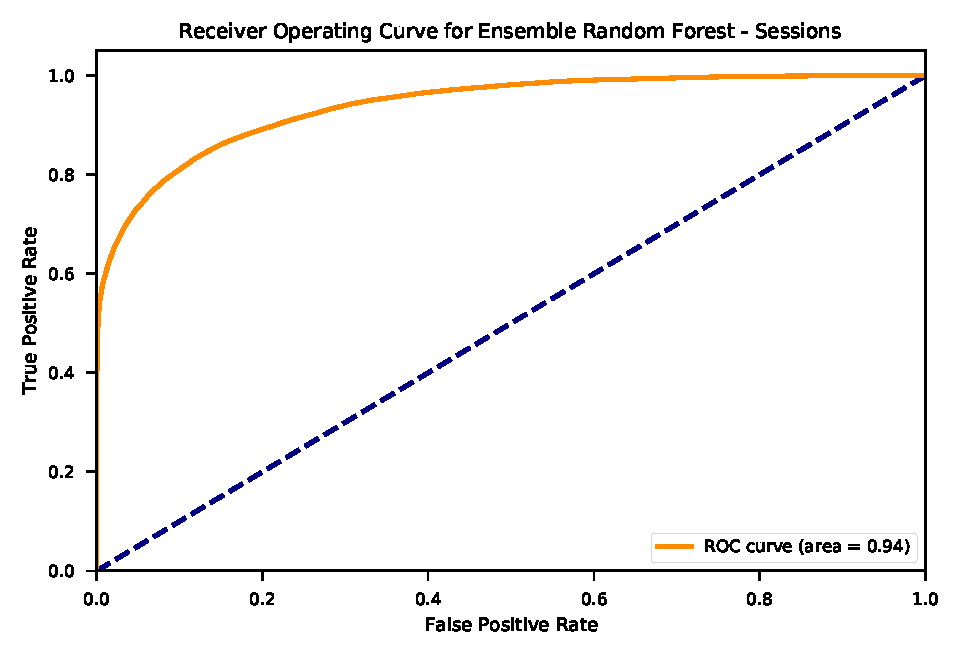
\includegraphics[width=0.80\linewidth]{images/sessions/roc_EnsembleRandomForestSessions.pdf}
    \caption{This figure shows the receiver operating curve and the respective area for the random forest classifier. The curve area is almost 1, showing that the cross-validation was a useful test.}
    \label{fig:session_random_forest_roc} 
\end{figure}

\begin{figure}[htbp]
    \centering
    \begin{subfigure}[b]{0.70\textwidth}
        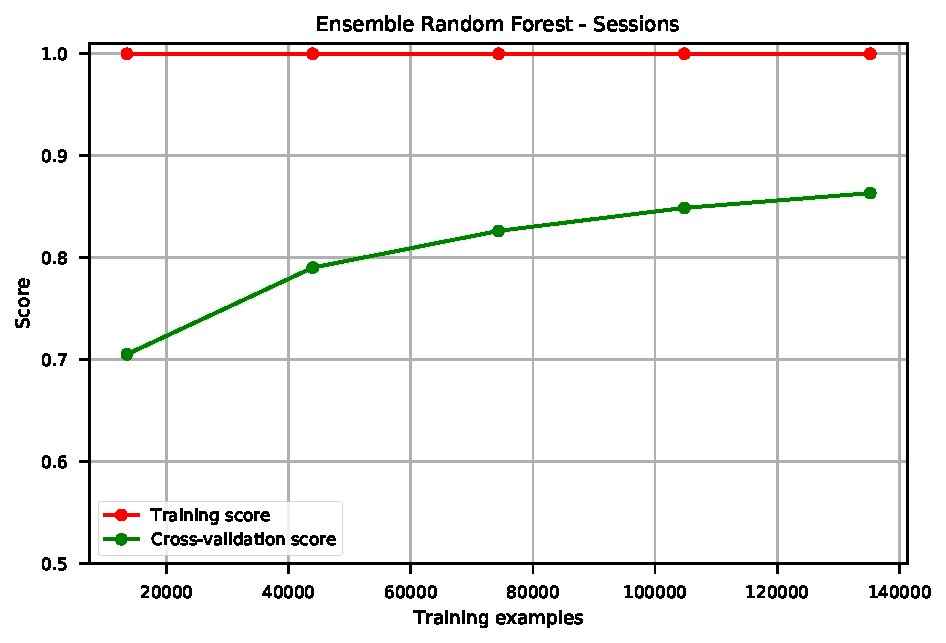
\includegraphics[width=\textwidth]{images/sessions/learning_curve_1_EnsembleRandomForestSessions.pdf}
        \caption{The cross validation score increases logarithmically.}
        \label{fig:learning_curve_1_EnsembleRandomForestSessions}
    \end{subfigure}
    \begin{subfigure}[b]{0.70\textwidth}
        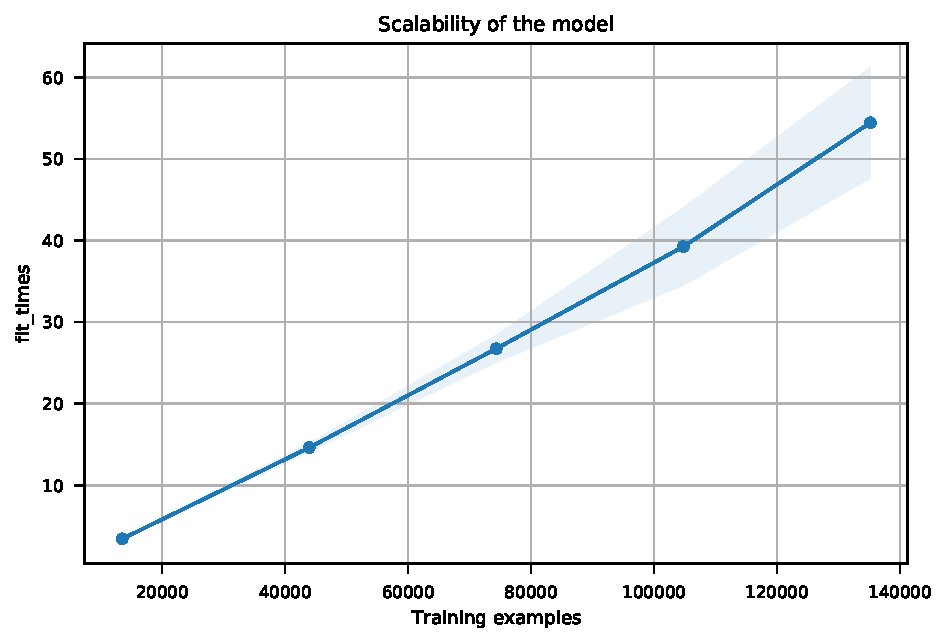
\includegraphics[width=\textwidth]{images/sessions/learning_curve_2_EnsembleRandomForestSessions}
        \caption{The scalability of the model increases linearly.}
        \label{fig:learning_curve_2_EnsembleRandomForestSessions}
    \end{subfigure}
    \begin{subfigure}[b]{0.70\textwidth}
        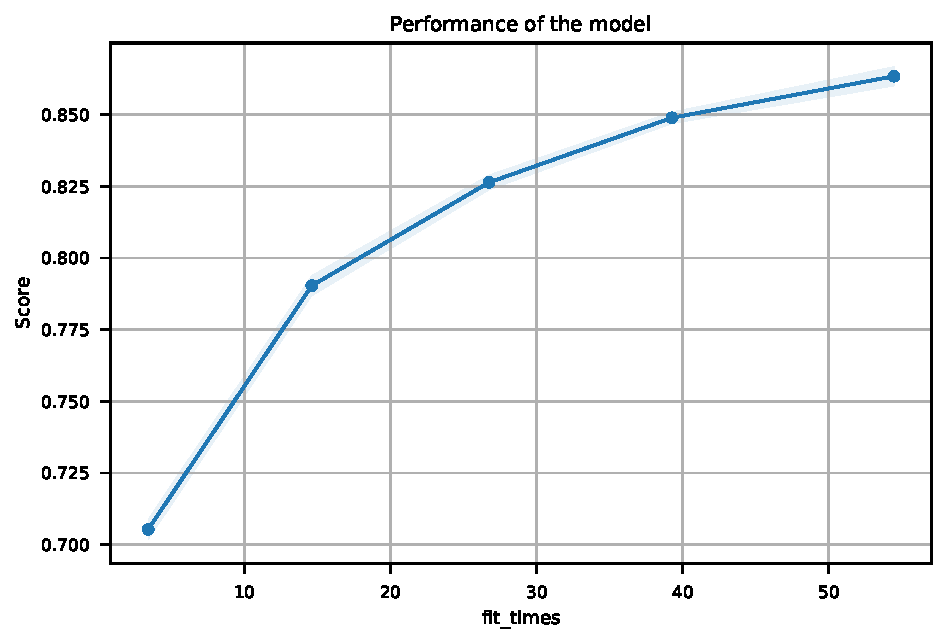
\includegraphics[width=\textwidth]{images/sessions/learning_curve_3_EnsembleRandomForestSessions}
        \caption{The performance of the model increases logarithmically.}
        \label{fig:learning_curve_3_EnsembleRandomForestSessions}
    \end{subfigure}
    \caption{This figure shows the performance of the random forest classifier during cross-validation. The score increases by a small factor as the training examples increase. It is not logarithmic as the original decision tree model. The fit time increases linearly with the training examples. The fit times increase logarithmically with the score.}\label{fig:session_random_forest_learning_curve}
\end{figure}

\chapter{Introduction and Debrief Scripts}
\begin{figure}[htb]
Thank you for agreeing to hear about what my project is about. The aim of this experiment is to determine whether a reliable method can be created to predict a person’s social anxiety by using their session activity. Session activity is defined as the applications used within sessions. A session is the time when a phone is unlocked. Past research indicates that an individual's application session data is a good indicator of cognitive health, and so we would like to see if we can apply that knowledge to learn more about social anxiety and apply it to further research.\newline\newline Participants are needed to provide data as the data cannot be synthesized. The experiment will involve you installing an Android application and enabling it to collect data in the background. You will additionally have to take a 20 question quiz which will tell you your social anxiety. This is the Social Interaction Anxiety Scale (SIAS) and is a widely-recognised self-report in social anxiety research. The application will show a persistent notification when data collection is enabled. This data is saved on the Android device. I will not need to observe you for the duration of the experiment. The application will collect data for a week. Once a week has passed, I will ask you to export the data from the device.\newline\newline The application does not test your ability in any way, and just passively collects data. In the end, this data will be analysed. The data is made up of usage statistics, such as applications used within sessions and application categories. The application will also collect location data and phone call duration times. This extra data is collected in order to compare with past research. I link your data with a unique identifier that is generated on the device. This unique identifier is not related to you or your device and I am not able to link you to your identifier. I have taken precautions by encrypting the data stored in the database as well as encrypting data transmit from phone to server and server to database. The server has a TLS certificate signed by Let's Encrypt. At the end of the study, the data will be deleted.\newline\newline I kindly ask you to leave location turned on and battery saver turned off during the duration of the study. This is to ensure that data is consistent and reliable. However I understand if you are not able to do this for the entire duration.\newline\newline During the experiment you are able to contact me at any time to opt out or report something out of the ordinary. You can either do this through the application settings or by directly contacting me. This study will not affect any other course or activity that you are currently enrolled in. If you agree to this study, I will send you the sign-up form, which will take your name, email, consent, and timestamp on submission. After that is signed, I will send you a link to the application file to install. Please do not hesitate to ask questions or contact me (Anguel Hristozov) at 2255541h@student.gla.ac.uk, or the project supervisor Matthew Chalmers at Matthew.Chalmers@glasgow.ac.uk.
    \caption{This is the introduction script that was shown to each participant before giving them the survey to agree to participate.}
    \label{fig:intro_script} 
\end{figure}


\begin{figure}[htb]
The aim of this experiment is to determine whether a reliable method can be created to predict a person’s social anxiety by using their session activity. Specifically,  If you would still like to proceed, please click the "Export Data" button on the main screen to send me your data. If at any point you would like me to remove your data, please fill out the form below and send me your identifier.\newline\newline Do you have any comments or questions about the experiment? Please do not hesitate to contact me at 2255541h@student.gla.ac.uk. Please take a note of this email as well as my supervisor's contact in case you have any further questions afterwards. Thank you for your help.\newline\newline The opt-out form is here: \url{https://forms.gle/Fd4iyFCN5vHLPRmE8}
    \caption{This is the debrief script that was shown to each participant after the user trial has finished.}
    \label{fig:debrief_script} 
\end{figure}

\chapter{Sign-Up, After Study, and Opt-Out Forms}
\begin{figure}[htb]
    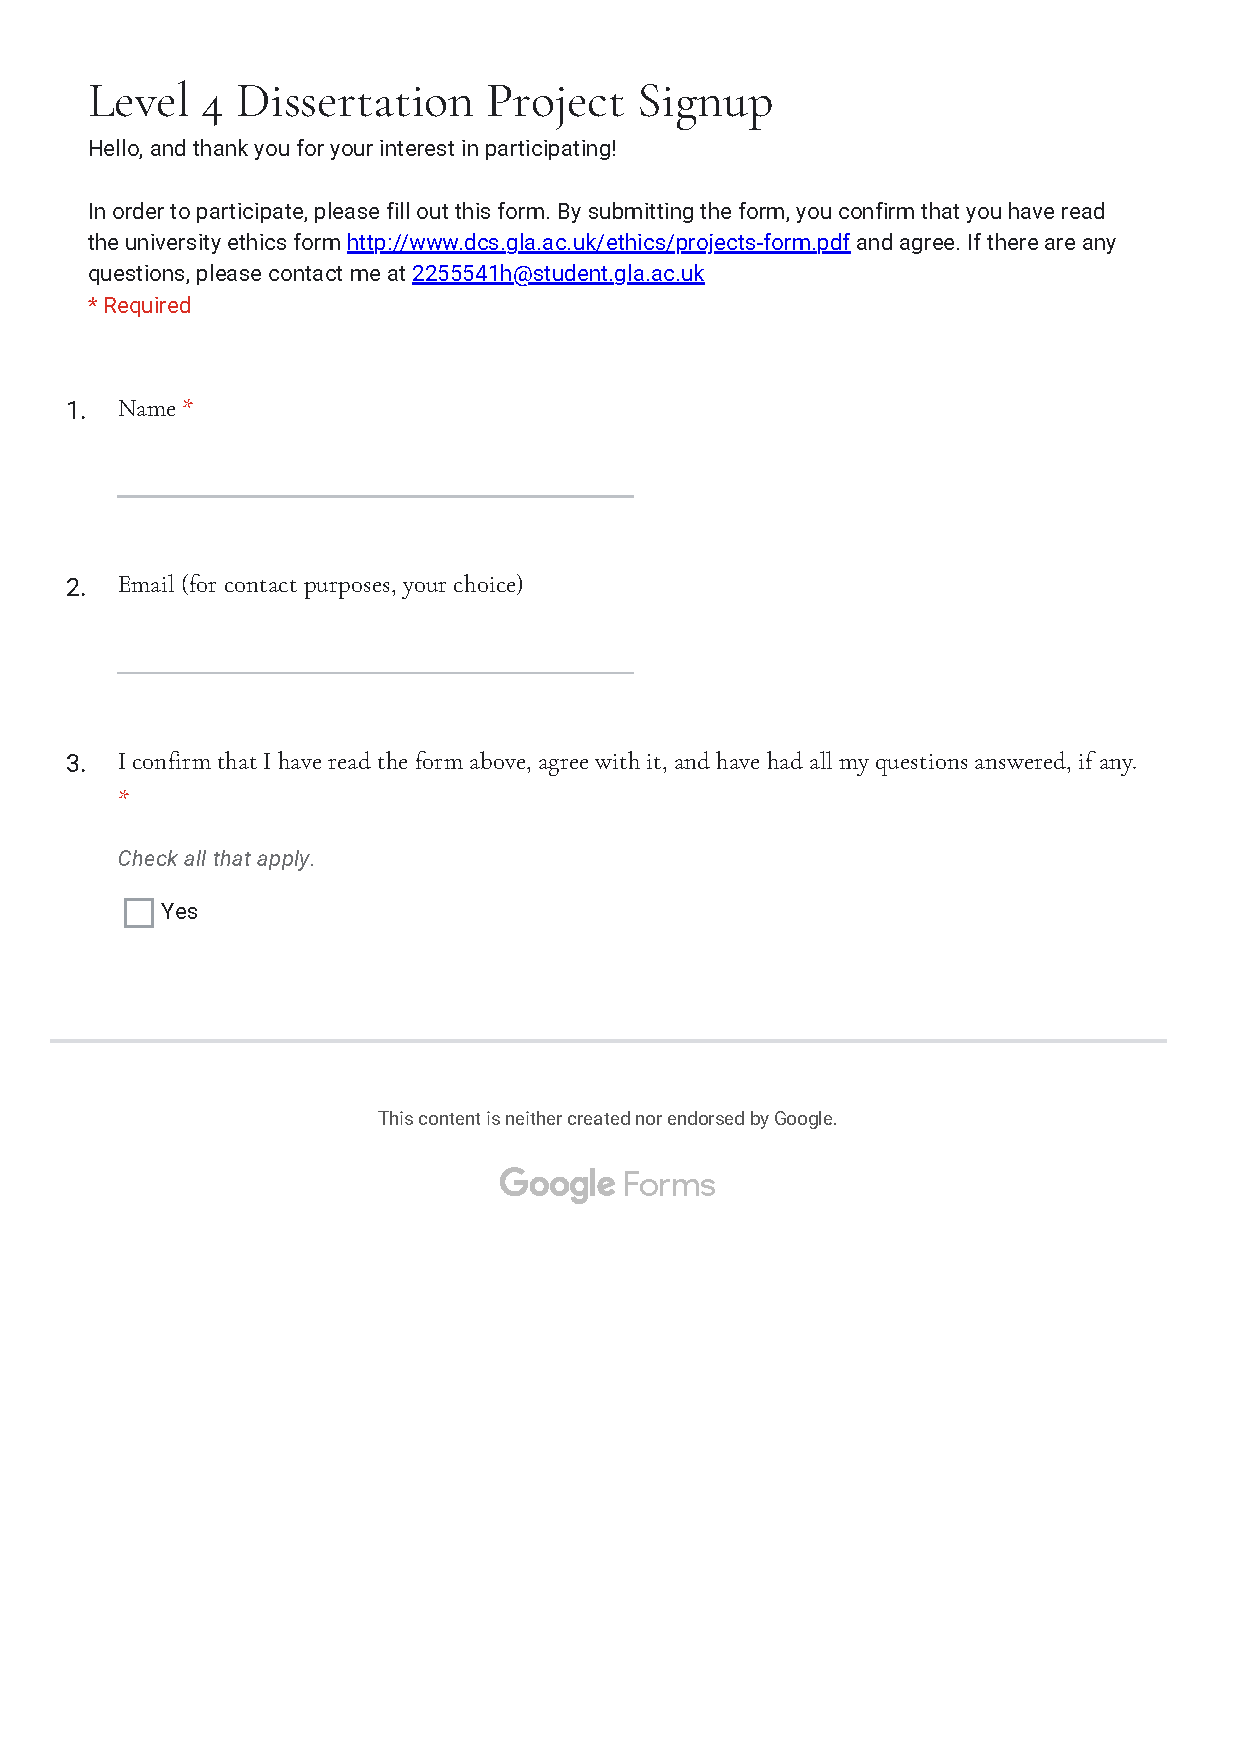
\includegraphics[width=\linewidth]{images/signup_form.pdf}
    \caption{This is the sign-up and consent form that was sent to every participant. Individuals had to agree otherwise they could not participate.}
    \label{fig:consent_form} 
\end{figure}

\begin{figure}[htb]
    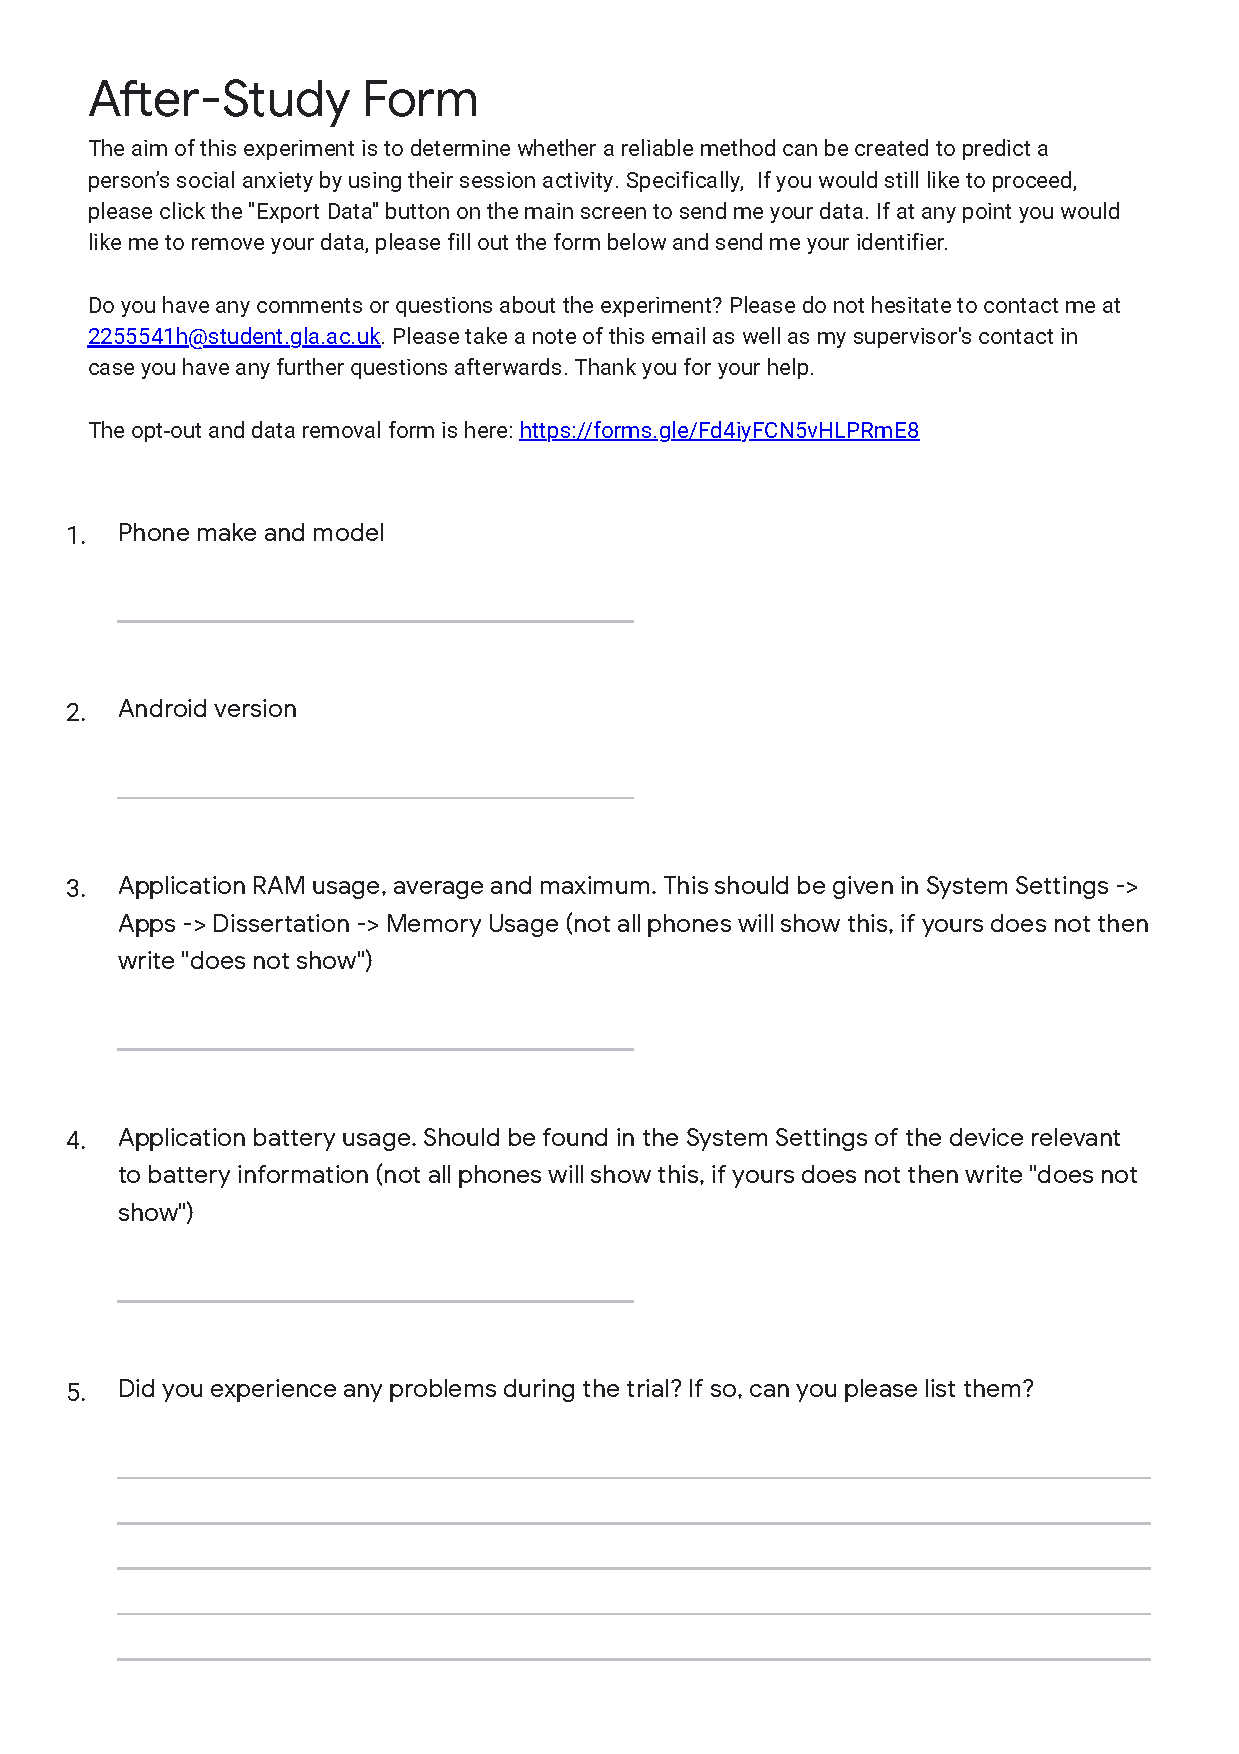
\includegraphics[width=\textwidth]{images/device_form_1.pdf}
    \caption{This is the first page of the form that was sent out to participants after the trial finished.}
    \label{fig:device_form1}
\end{figure}

\begin{figure}[htb]
    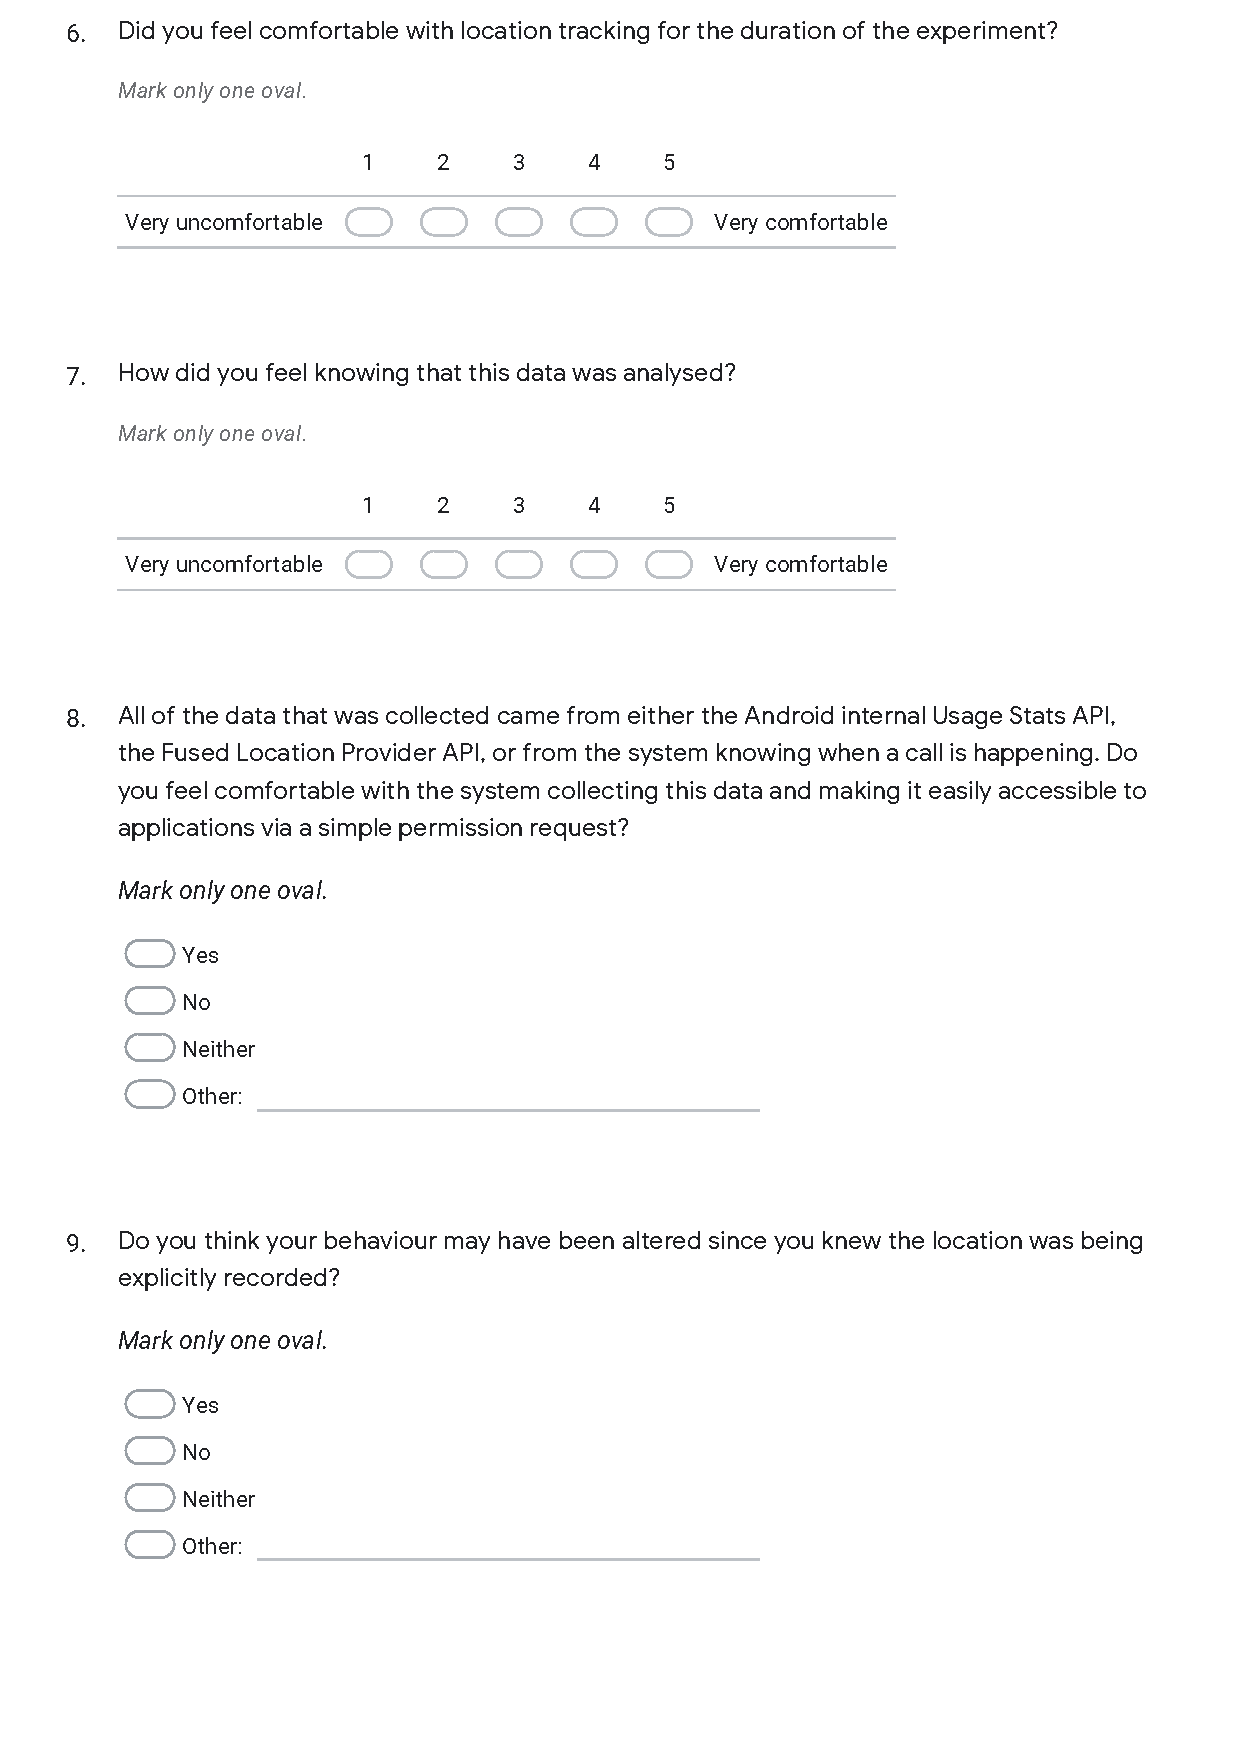
\includegraphics[width=\textwidth]{images/device_form_2.pdf}
    \caption{This is the first page of the form that was sent out to participants after the trial finished.}
    \label{fig:device_form2}
\end{figure}

\begin{figure}[htb]
    \includegraphics[width=\textwidth]{images/device_form_3.pdf}
    \caption{This is the first page of the form that was sent out to participants after the trial finished.}
    \label{fig:device_form3}
\end{figure}

\begin{figure}[htb]
    \includegraphics[width=\linewidth]{images/optout_form.pdf}
    \caption{This is the opt-out form.}
    \label{fig:opt_out} 
\end{figure}

\chapter{Participant Comfort Level Graphs} \label{app_appendix}
\begin{figure}[htb]
    \centering
    \includegraphics[width=\linewidth]{images/survey/usage_stats.pdf}
    \caption{This figure shows the comfort level of participants with knowing that their usage data is readily available. A majority are comfortable with it but it is important to note that a significant portion are unsure. This suggests that they do not yet fully understand the ramifications of having such data available or that they were not aware of it.}
    \label{fig:usage_stats} 
\end{figure}

\begin{figure}[htb]
    \centering
    \includegraphics[width=\linewidth]{images/survey/behaviour_change.pdf}
    \caption{This figure shows if people noticed a change in behaviour knowing that their usage data was being collected. It is important to note that an overwhelming majority report no, signifying that there is very little bias in the data due to altered behaviour.}
    \label{fig:behaviour_change} 
\end{figure}

\begin{figure}[htb]
    \centering
    \includegraphics[width=\linewidth]{images/survey/location_tracking_comfort.pdf}
    \caption{This figure shows the comfort level of participants with knowing that their data location is tracked. Overall a majority is comfortable}
    \label{fig:location_tracking_comfort} 
\end{figure}

\begin{figure}[htb]
    \centering
    \includegraphics[width=\linewidth]{images/survey/data_analysis_comfort.pdf}
    \caption{This figure shows the comfort level of participants with knowing that their data is to be analysed. Overall a majority is comfortable.}
    \label{fig:data_analysis_comfort} 
\end{figure}

\chapter{Signed Ethics Form}
\begin{figure}[htb]
    \centering
    \includegraphics[width=\linewidth]{images/signed_ethics_form_1-1.pdf}
    \caption{This is the first page of the ethics form.}
    \label{fig:ethics_form_1} 
\end{figure}

\begin{figure}[htb]
    \centering
    \includegraphics[width=\linewidth]{images/signed_ethics_form_2-end.pdf}
    \caption{This is the second signed page of the ethics form. It has been digitally signed as there was no option to get to a printer and scan it due to extraordinary events at the time.}
    \label{fig:ethics_form_2} 
\end{figure}

\end{appendices}

%==================================================================================================================================
%   BIBLIOGRAPHY   

% The bibliography style is agsm (Harvard)
% The bibliography always appears last, after the appendices.

\bibliographystyle{agsm}

% Force the bibliography not to be numbered
\renewcommand{\thechapter}{0} 
\bibliography{l4proj}

\end{document}
